\chapter{Testování hypotéz}

\section{Základní pojmy}

\begin{definition}[Statistiká hypotéza]
Statistickou větou se rozumí tvrzení a pravděpodobnostním rozdělení jedné nebo více náhodných veličin. Jestliže statistická hypotéza plně specifikuje toto pravděpodobnostní rozdělení, nazýváme ji jednoduchou statistickou hypotézou. V opačném případě mluvíme o tzv. složené statistické hypotéze.
\end{definition}

\begin{example}
Uvažujme náhodný výběr $X_1, ..., X_n$ z populace $f(x, \theta) = \phi_{\theta, 25}(x)$. Statistickou hypotézu, že střední hodnota tohoto normálního rozdělení je menší nebo rovna 17, zapisujeme jako $\mathscr{H}: \theta \le 17$. Takto definovaná hypotéza je složená, protože plně nespecifikuje normální rozdělení. Naproti tomu hypotéza, že střední hodnota normálního rozdělení je rovna 17, tj. $\mathscr{H}: \theta = 17$, je jednoduchou statistickou hypotézou.
\end{example}

\begin{definition}[Test statistiké hypotézy]
Testem statistické hypotézy $\mathscr{H}$ s rozumí pravidlo, na základě kterého se tato hypotéza přijme popř. zamítne. Test statistické hypotézy značíme jako $\mathscr{T}$.
\end{definition}

\begin{example}
Uvažujme náhodný výběr $X_1, ..., X_n$ z populace $f(x, \theta) = \phi_{\theta, 25}(x)$. Definujme statistickou hypotézu $\mathscr{H}: \theta \le 17$. Jedním z možných testů této hypotézy je zamítnutí $\mathscr{H}$, jestliže $\overline{X} > 17 + 5 / \sqrt{n}$.
\end{example}

Test hypotézy může být náhodný popř. nenáhodný. Test $\mathscr{T}$ z výše uvedeného příkladu je testem nenáhodným. Alternativní test $\mathscr{T}'$ hypotézy $\mathscr{H}$ z výše uvedeného příkladu by mohl spočívat v hodu mincí a následném zamítnutí $\mathscr{H}$, pokud by padla panna. Takovýto test by byl testem náhodným.

Stejně jako v předchozím textu budeme $\mathfrak{X}$ používat pro označení výběrového prostoru pozorování, tj. $\mathfrak{X} = \{(x_1, ..., x_n) : (x_1, ..., x_n) ~ \textit{představují všechny možné kombinace náhodných veličin}~(X_1, ..., X_n)\}$. 

\begin{definition}[Nenáhodný test a kritický region]
Uvažujme test $\mathscr{T}$ statistické hypotézy $H$, který tuto hypotézu zamítne, jestliže $(x_1, ..., x_n) \in C_{\mathscr{T}}$, kde $C_{\mathscr{T}}$ je podmnožinou $\mathfrak{X}$. Pak test $\mathscr{T}$ nazýváme nenáhodným testem a $C_{\mathscr{T}}$ jeho kritickým regionem.
\end{definition}

\begin{example}
Uvažujme náhodný výběr $X_1, ..., X_n$ z populace $f(x, \theta) = \phi_{\theta, 25}(x)$, tj. $\mathfrak{X}$ je $n$-rozměrný euklidovský prostor. Dále uvažujme hypotézu $\mathscr{H}: \theta \le 17$ a test $\mathscr{T}$, který zavrhuje tuto hypotézu pro $\overline{x} > 17 + 5 / \sqrt{n}$. Pak je $\mathscr{T}$ nenáhodným testem a $C_{\mathscr{T}} = \{(x_1, ..., x_n): \overline{x} > 17 + 5 / \sqrt{n} \}$.
\end{example}

V případě nenáhodného testu $\mathscr{T}$ hypotézy $\mathscr{H}$ je tak $\mathfrak{X}$ rozděleno na $C_{\mathscr{T}}$ a $\overline{C}_{\mathscr{T}}$ takové, že pro $(x_1, ..., x_n) \in C_{\mathscr{T}}$ je $\mathscr{H}$ zamítnuto. Nenáhodný test je tak specifikován svým kritickým regionem.

\begin{definition}[Náhodný test]
Test $\mathscr{T}$ hypotézy $\mathscr{H}$ je náhodný, jestliže je $\mathscr{T}$ definován funkcí\
\begin{equation*}
\psi_{\mathscr{T}}(x_1, ..., x_n) = P[\mathscr{H}~\textit{je zamítnuta pro realizaci náhodného výběru}~(x_1, ..., x_n)]
\end{equation*}
Tuto funkci nazýváme kritickou funkcí testu $\mathscr{T}$.
\end{definition}

Při aplikaci náhodného testu $\mathscr{T}$ hypotézy $\mathscr{H}$ je pro realizovaný náhodný výběr $(x_1, ..., x_n)$ ohodnocena funkce $\psi_{\mathscr{T}}(x_1, ..., x_n)$. Následně je proveden pomocný výběr z Bernoulliho rozdělení s pravděpodobností úspěchu $\psi_{\mathscr{T}}(x_1, ..., x_n)$. Jestliže tento výběr indikuje ``úspěch'', je $\mathscr{H}$ zamítnuta. Z tohoto popisu je zřejmé, že náhodné testy nejsou v praxi příliš používané. V některých případech je $\mathfrak{X}$ rozděleno na tři části, kde pro jednu je $\mathscr{H}$ přijato, pro druhou je $\mathscr{H}$ zamítnuto a pro třetí, která představuje ``šedou zónu'', je aplikován náhodný test. Situaci ilustruje následující příklad.

\begin{example}
Uvažujme náhodný výběr $X_1, ..., X_{10}$ z populace $f(x, \theta) = \theta^x(1 - \theta)^{1 - x}$ pro $x = 0, 1$. Předpokládejme, že chceme testovat hypotézu $\mathscr{H}: \theta < \frac{1}{2}$. Jedním z možných testů je $\mathscr{T}$ definovaný jako
\begin{enumerate}
\item zamítni $\mathscr{H}$, jestliže $\sum_{i = 1}^{10} x_i > 5$,
\item přijmi $\mathscr{H}$, jestliže $\sum_{i = 1}^{10} x_i < 5$ a
\item hoď mincí\footnote{Hod mincí zde zastupuje pomocný výběr z Bernoulliho rozdělení.} a rozhodni, jestliže $\sum_{i = 1}^{10} x_i = 5$
\end{enumerate}
Test $\mathscr{T}$ tedy rozděluje $\mathfrak{X}$ na tři části $A, B$ a $C$, kde
\begin{gather*}
A = \left\{(x_1, ..., x_{10}: \sum_{i = 1}^{10}x_i < 5)\right\}\\
B = \left\{(x_1, ..., x_{10}: \sum_{i = 1}^{10}x_i = 5)\right\}\\
C = \left\{(x_1, ..., x_{10}: \sum_{i = 1}^{10}x_i > 5)\right\}\\
\end{gather*}
Kritická funkce testu $\mathscr{T}$ je pak definována jako
\begin{equation*}
\psi_{\mathscr{T}(x_1, ..., x_n)} =
\begin{cases}
1 ~ \textit{pro} ~ (x_1, ..., x_{10}) \in C\\
\frac{1}{2} ~ \textit{pro} ~ (x_1, ..., x_{10}) \in B\\
0 ~ \textit{pro} ~ (x_1, ..., x_{10}) \in A
\end{cases}
\end{equation*}
\end{example}

V předchozím textu jsme uvedli, že nenáhodný test je specifikován svým kritickým regionem a že stejnou úlohu v případě náhodného testu pak plní kritická funkce. Platí, že libovolná funkce $\psi(\cdot, ..., \cdot)$ s definičním oborem $\mathfrak{X}$ a oborem hodnot $[0, 1]$ je možnou kritickou funkcí, která definuje náhodný test.

Jestliže je test $\mathscr{T}$ definován kritickou funkcí
\begin{equation*}
\psi_{\mathscr{T}}(x_1, ..., x_n) =
\begin{cases}
1 ~ \textit{pro} ~ (x_1, ..., x_n) \in C_{\mathscr{T}}\\
0 ~ \textit{v ostatních případech}
\end{cases}
\end{equation*}
pak je $\mathscr{T}$ nenáhodným testem s kritickým regionem $C_{\mathscr{T}}$.

Při testování hypotéz se rozhodujeme mezi tzv. nulovou hypotézou $\mathscr{H}_0$ a alternativní hypotézou $\mathscr{H}_1$. Logika rozhodování je taková, že je-li $\mathscr{H}_0$ zamítnuta, pak je přijata $\mathscr{H}_1$ a naopak. Při tomto postupu se můžeme dopustit dvou druhů chyb.

\begin{definition}[Typy chyb při testování hypotéz]
Chyba, které se dopustíme, jestliže zamítneme $\mathscr{H}_0$, která je ve skutečnosti pravdivá, je tzv. chybou typu I. Naopak přijetím $\mathscr{H}_0$, která je však ve skutečnosti nepravdivá, se dopouštíme chyby typu II. Velikosti chyb typu I a II jsou definovány pravděpodobnostmi, že se těchto chyb dopustíme.
\end{definition}

Jestliže je pravděpodobnostní rozdělení, ze kterého provádíme náhodný výběr, funkcí parametru $\theta$, kde $\theta \in \overline{\underline{\Theta}}$, pak lze každému testu přiřadit tzv. funkci charakteristické veličiny.

\begin{definition}[Funkce charakteristické veličiny]
Uvažujme test $\mathscr{T}$ nulové hypotézy $\mathscr{H}_0$. Funkce charakteristické veličiny testu $\mathscr{T}$ je označována $\pi_{\mathscr{T}}(\theta)$ a je definována jako pravděpodobnost zamítnutí $\mathscr{H}_0$, jestliže pravděpodobností rozdělení, ze kterého byl prováděn náhodný výběr, je funkcí parametru $\theta$.
\end{definition}

Funkce charakteristické veličiny plní stejnou roli jako MSE v případě bodového odhadu - v následujícím textu bude představovat standardní nástroj pro porovnání daného testu s alternativními testy. Z definice je zřejmé, že ideální funkce charakteristické veličiny nabývá nulové hodnoty pro $\theta$, která odpovídají nulové hypotéze, a jednotkové hodnoty pro $\theta$, která odpovídají alternativní hypotéze.

Platí, že $\pi_{\mathscr{T}}(\theta) = P_{\mathscr{T}}[\textit{zamítnutí}~\mathscr{H}_0]$, kde $\theta$ představuje skutečnou hodnotu parametru. Jestliže je $\mathscr{T}$ nenáhodným testem, pak $\pi_{\mathscr{T}}(\theta) = P_{\theta}[(X_1, ..., X_n) \in C_{\mathscr{T}}]$, kde $C_{\mathscr{T}}$ je kritickým regionem testu $\mathscr{T}$. Jestliže je $\mathscr{T}$ náhodným testem s kritickou funkcí $\psi_{\mathscr{T}}(\cdot, ..., \cdot)$, pak
\begin{multline*}
\pi_{\mathscr{T}} = P_{\mathscr{T}}[\textit{zamítnutí}~\mathscr{H}_0]\\
= \int \cdots \int P[\textit{zamítnutí}~\mathscr{H}_0 | x_1, ..., x_n]f_{X_1, ..., X_n}(x_1, ..., x_n; \theta) \prod_{i = 1}^n d x_i\\
= \int \cdots \int \psi_{\mathscr{T}}(x_1, ..., x_n)f_{X_1, ..., X_n}(x_1, ..., x_n; \theta)\prod_{i = 1}^n d x_i = E_{\theta}[\psi_{\mathscr{T}}(X_1, ..., X_n)]
\end{multline*}
Analogické odvození lze provést také v případě nespojité náhodné veličiny.

\begin{example}
Uvažujme náhodný výběr $X_1, ..., X_n$ z populace $f(x, \theta) = \phi_{\theta, 25}(x)$. Uvažujme nulovou hypotézu $\mathscr{H}_0: \theta \le 17$ a test $\mathscr{T}$, který zavrhuje $\mathscr{H}_0$, jestliže $\overline{X} > 17 + 5 / \sqrt{n}$. Funkce charakterické veličiny je dána rovnicí
\begin{equation*}
\pi_{\mathscr{T}}(\theta) = P_{\theta}\left[\overline{X} > 17 + \frac{5}{\sqrt{n}} \right] = 1 - \Phi\left(\frac{17 + 5 / \sqrt{n} - \theta}{5 / \sqrt{n}}\right)
\end{equation*}
Pro $n = 25$ je $\pi_{\mathscr{T}}(\theta)$ ilustrována obrázkem (\ref{power-function}). Funkce charakteristiké veličiny indikuje, nakolik je daný test spolehlivý. Jestliže je v našem konkrétním případě $\theta$ větší než 20, pak test $\mathscr{T}$ správně zamítne $\mathscr{H}_0$. Naopak, jestliže je $\theta$ menší než 16, pak test $\mathscr{T}$, opět správně, s vysokou pravděpodobností $\mathscr{H}_0$ nezamítne. Jestliže je však $17 < \theta < 18$, je pravděpodobnost zamítnutí $\mathscr{H}_0$ na základě testu $\mathscr{T}$ méně než poloviční, ačkoliv je hypotéza $\mathscr{H}_0$ nepravdivá.
\end{example}

\begin{figure}[htp]
\centering
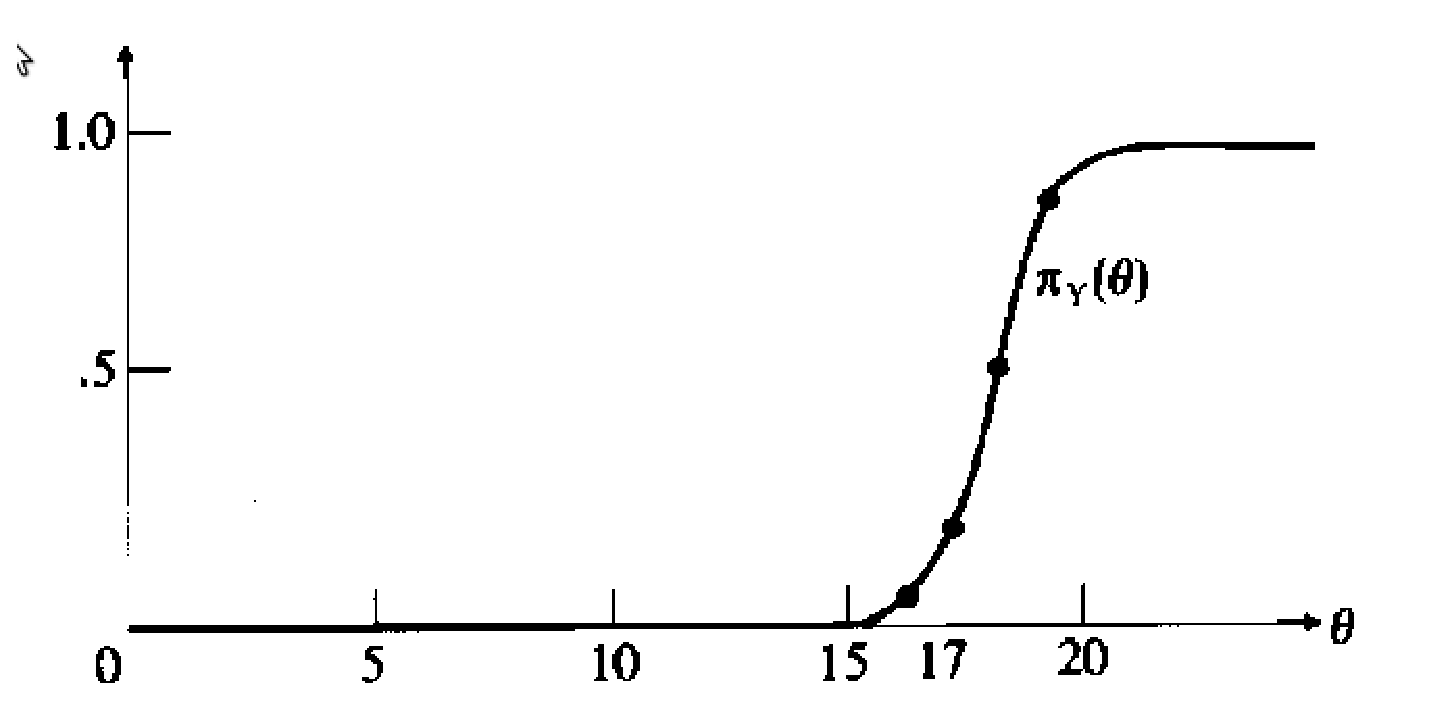
\includegraphics[scale = 0.5]{pictures/power_function.eps}
\caption{Funkce charakteristické veličiny}
\label{power-function}
\end{figure}

\begin{definition}[Velikost testu]
Uvažujme test $\mathscr{T}$ hypotézy $\mathscr{H}_0: \theta \in \overline{\underline{\Theta}}_0$, kde $\overline{\underline{\Theta}}_0 \subset \overline{\underline{\Theta}}$. Velikost testu $\mathscr{T}$ je definována jako $\sup_{\theta \in \overline{\underline{\Theta}}_0}[\pi_{\mathscr{T}}(\theta)]$. Velikost nenáhodného testu je někdy také nazývána velikostí kritického regionu.
\end{definition}

\begin{example}
Uvažujme náhodný výběr $X_1, ..., X_n$ z populace $f(x, \theta) = \phi_{\theta, 25}(x)$. Dále uvažujme hypotézu $\mathscr{H}_0: \theta \le 17$ a test $\mathscr{T}$, který zavrhuje $\mathscr{H}_0$ jestliže $\overline{X} > 17 + 5 / \sqrt{n}$. Platí $\overline{\underline{\Theta}}_0 = \{\theta: \theta \le 17\}$ a velikost testu $\mathscr{T}$ je
\begin{equation*}
\sup_{\theta \in \overline{\underline{\Theta}}_0}[\pi_{\mathscr{T}}(\theta)] = \sup_{\theta \le 17}\left[1 - \Phi\left(\frac{17 + 5 / \sqrt{n} - \theta}{5 / \sqrt{n}}\right)\right] = 1 - \Phi(1) \approx 0.159
\end{equation*}
\end{example}

\begin{theorem}
Uvažujme náhodný výběr $X_1, ..., X_n$ z populace $f(x, \theta)$, kde $\theta \in \overline{\underline{\Theta}}$ a soubor dostatečných statistik $S_1 = \mathfrak{s}_1(X_1, ..., X_n), ..., S_r = \mathfrak{s}_r(X_1, ..., X_n)$. Pak pro libovolný test $\mathscr{T}$ s kritickou funkcí $\psi_{\mathscr{T}}(X_1, ..., X_n)$ existuje test $\mathscr{T}'$ s kritickou funkcí $\psi_{\mathscr{T}'}(S_1, ..., S_r)$, která splňuje $\pi_{\mathscr{T}}(\theta) = \pi_{\mathscr{T}'}(\theta)$ pro všechna $\theta \in \overline{\underline{\Theta}}$.
\end{theorem}

\begin{proof}
Definujme $\psi_{\mathscr{T}'}(s_1, ..., s_r) = E[\psi_{\mathscr{T}}(X_1, ..., X_n)|S_1 = s_1, ..., S_r = s_r]$, pak $\psi_{\mathscr{T}'}$ je kritickou funkcí. Dále platí $\pi_{\mathscr{T}'}(\theta) = E_{\theta}[\psi_{\mathscr{T}'}(S_1, ..., S_r)] = E_{\theta}[E[\psi_{\mathscr{T}}(X_1, ..., X_n)|S_1, ..., S_r]] = E_{\theta}[\psi_{\mathscr{T}}(X_1, ..., X_n)] = \pi_{\mathscr{T}}(\theta)$.
\end{proof}

Z výše uvedené věty vyplývá, že pro libovolný test existuje alternativní test založený pouze na souboru dostatečných statistik a že tento test má stejnou funkci charakteristické veličiny jako test původní. Při našem pátrání po vhodném testu se tak můžeme omezit pouze na testy založených právě na souboru dostatečných statistik.

\section{Testování jednoduchých hypotéz}

\begin{definition}[Jednoduchý věrohodnostní poměrový test]
Uvažujme náhodný výběr $X_1, ..., X_n$, o kterém víme, že pochází buď z populace $f_0(\cdot)$ nebo $f_1(\cdot)$. Test $\mathscr{T}$, který testuje $\mathscr{H}_0: X_i \sim f_0(\cdot)$ proti $\mathscr{H}_1: X_i \sim f_1(\cdot)$, je nazýván jednoduchým věrohodnostním poměrovým testem, jestliže je definován jako
\begin{enumerate}
\item zamítni $\mathscr{H}_0$, jestliže $\lambda < k$,
\item přijmi $\mathscr{H}_0$, jestliže $\lambda > k$,
\item přijmi / zamítni $\mathscr{H}_0$ popř. rozhodni na základě náhodného testu, jestliže $\lambda = k$
\end{enumerate}
kde
\begin{equation*}
\lambda = \lambda(x_1, ..., x_n) = \frac{\prod_{i = 1}^n f_0(x_i)}{\prod_{i = 1}^n f_1(x_i)} = \frac{L_0(x_1, ..., x_n)}{L_1(x_1, ..., x_n)} = \frac{L_0}{L_1}
\end{equation*}
a $k$ je nezáporná konstanta. Připomeňme, že $L_j = L_j(x_1, ..., x_n)$ je funkce maximální věrohodnosti pro náhodný výběr z populace $f_j(\cdot)$.
\end{definition}

Pro fixní $k$ tedy test zavrhuje $\mathscr{H}_0$ pro nízké hodnoty $\lambda$ a naopak. Výsledek testu tedy zavisí na zvolené hodnotě $k$.

Jednoduchý věrohodnostní poměrový test je v souladu s intuicí. Navíc lze očekávat, že ``optimální'' test bude mít podobu právě jednoduchého věrohodnostního poměrového testu. K hledání ``optimálního'' testu pro jednoduché hypotézy lze přistoupit dvěma způsoby - prvním z nich je koncept tzv. nejsilnějšího testu a druhý spočívá ve využití ztrátové funkce.

\subsection{Nejsilnější test}

Uvažujme náhodný výběr $X_1, ..., X_n$, o kterém víme, že pochází buď z populace $f_0(\cdot)$ nebo $f_1(\cdot)$, kde $f_0(x) = f(x, \theta_0)$ a $f_1(x) = f(x, \theta_1)$ a $\theta_0$ a $\theta_1$ jsou známé konstanty. To znamená, že $\overline{\underline{\Theta}} = \{\theta_0, \theta_1\}$ je prostor, který se skládá z pouchých dvou bodů. Testujme hypotézu $\mathscr{H}_0: \theta = \theta_1$ proti hypotéze $\mathscr{H}_1: \theta = \theta_1$. Tomuto testu lze přiřadit funkci charakteristické veličiny $\pi_{\mathscr{T}}(\theta)$. Dobrý test je takový, pro který je $\pi_{\mathscr{T}}(\theta_0) = P[\textit{zamítnutí} ~ \mathscr{H}_0|\mathscr{H}_0 ~ \textit{je pradivá}]$ malé (ideálně rovno nule) a $\pi_{\mathscr{T}}(\theta_0) = P[\textit{zamítnutí} ~ \mathscr{H}_0|\mathscr{H}_0 ~ \textit{je nepradivá}]$ vysoké (ideálně rovno jedné).  $\pi_{\mathscr{T}}(\theta_0)$ odpovídá chybě typu I a $1 - \pi_{\mathscr{T}}(\theta_1) = P[\textit{přijetí} ~ \mathscr{H}_0 | \mathscr{H}_0 ~ \textit{je nepravdivá}]$ odpovídá chybě typu II. Naším cílem je minimalizovat obě chyby. Možných postupů je několik.

\begin{definition}[Nejsilnější test]
Test $\mathscr{T}^*$, který testuje $\mathscr{H}_0: \theta = \theta_0$ proti $\mathscr{H}_1: \theta = \theta_1$ je nejsilnějším testem velikosti $\alpha$, kde $0 < \alpha < 1$, jestliže
\begin{enumerate}
\item $\pi_{\mathscr{T}^*}(\theta_0) = \alpha$
\item $\pi_{\mathscr{T}^*}(\theta_1) \ge \pi_{\mathscr{T}}(\theta_1)$ pro libovolný alternativní test $\mathscr{T}$, pro který platí $\pi_{\mathscr{T}}(\theta_0) \le \alpha$.
\end{enumerate}
\end{definition}

Důvod, proč fixujeme velikost chyby typu I na úroveň $\alpha$\footnote{$\alpha$ je nastaveno zpravidla na nízkou úroveň - obvyklé hodnoty jsou 0.01 a 0.05.} zatímco velikost chyby typu II nikoliv, je skutečnost, že nulová a alternativní hypotéza jsou zpravidla formulovány tak, že realizace chyby typu I má závažnější následky než realizace chyby typu II.

\begin{theorem}[Neyman-Pearsonova]
Uvažujme náhodný výběr $X_1, ..., X_n$ z populace $f(x, \theta)$, kde $\theta$ nabývá hodnoty $\theta_0$ nebo $\theta_1$. Předpokládejme, že $\alpha$, kde $0 < \alpha < 1$, je fixní a známé. Nechť $k^*$ je pozitivní konstanta a $C^*$ je podmnožina $\mathfrak{X}$, která splňuje
\begin{enumerate}
\item $P_{\theta_0}[(X_1, ..., X_n) \in C^*] = \alpha$
\item $\lambda = \frac{L(\theta_0; x_1, ..., x_n)}{\theta_1; x_1, ..., x_n} = \frac{L_0}{L_1} \le k^*$ pro $(x_1, ..., x_n) \in C^*$
\item  $\lambda \ge k^*$ pro $(x_1, ..., x_n) \in \overline{C}^*$
\end{enumerate}
Pak je test $\mathscr{T}^*$, který je charakterizován kritickým regionem $C^*$, nejsilnějším testem velikosti $\alpha$ pro testování $\mathscr{H}_0: \theta = \theta_0$ proti $\mathscr{H}_1: \theta = \theta_1$. Připomeňme, že $L_j = L(\theta_j; x_1, ..., x_n) = \prod_{i = 1}^n f(x_i, \theta_j)$ pro $j = 0, 1$. $\overline{C}^*$ je doplněk k $C^*$, tj. $\overline{C}^* = \mathfrak{X} - C^*$
\end{theorem}

\begin{proof}
Předpokládejme, že existují taková $k^*$ a $C^*$, která splňují podmínky (1) až (3) výše uvedené věty. Uvažujme alternativní test $\mathscr{T}$ se silou alespoň $\alpha$ a kritickým regionem $C$, tj. $P_{\theta_0}[(X_1, ..., X_n) \in C] \le \alpha$.

V následujícím textu budeme pro libovolné $R \subset \mathfrak{X}$ namísto $\int \cdots \int_{R}\left[\prod_{i = 1}^n f(x_i, \theta_j)dx_i\right]$ používat zkrácený zápis $\int_R L_j$, kde $j = 0, 1$. Ze zápisu vyplývá, že $f_0(\cdot)$ a $f_1(\cdot)$ jsou pravděpodobnostní funkce spojité náhodné veličiny. Stejný důkaz nicméně platí také pro nespojité náhodné veličiny.

Musíme dokázat $\pi_{\mathscr{T}^*}(\theta_1) \ge \pi_{\mathscr{T}}(\theta_1)$, což je ekvivalentní důkazu $\int_{C^*} L_1 \ge \int_C L_1$. Následující postup ilustruje obrázek (\ref{most-power-test}). Platí
\begin{equation*}
\int_{C^*}L_1 - \int_C L_1 = \int_{C^* \overline{C}}L_1 - \int_{C \overline{C}^*}L_1 \le \frac{1}{k^*}\int_{C^* \overline{C}}L_0 - \frac{1}{k^*}\int_{C \overline{C}^*}L_0
\end{equation*}
protože $L_1 \ge \frac{L_0}{k^*}$ na množině $C^*$ (a tím pádem také na množině $C^* \overline{C}$) a $L_1 \le \frac{L_0}{k^*}$ neboli $-L_1 \ge -\frac{L_0}{k^*}$ na množině $\overline{C}^*$ (a tím pádem také na množině $C \overline{C}^*$). Nicméně
\begin{multline*}
\frac{1}{k^*}\left(\int_{C^* \overline{C}}L_0 - \int_{C\overline{C}^*}L_0\right) = \frac{1}{k^*}\left(\int_{C^*\overline{C}}L_0 - \int_{C^* C}L_0 + \int_{C^* C}L_0 - \int_{C \overline{C}^*}L_0\right)\\
= \frac{1}{k^*}\left(\int_{C^*} L_0 - \int_C L_0 \right) = \frac{1}{k^*}(\alpha - \textit{velikost testu} ~ \mathscr{T})
\end{multline*}
což implikuje $\int_{C^*}L_1 - \int_C L_1 \ge 0$.
\end{proof}

\begin{figure}[htp]
\centering

\includegraphics[scale = 0.5]{pictures/most_powerful_test.eps}
\caption{Ilustrační obrázek}
\label{power-function}
\end{figure}

Obecně platí, že ne vždy musí existovat $k^*$ a $C^*$, která splňují podmínky Neyman-Pearsovy věty. V takovém případě  Neyman-Pearsovy věta není schopná dát nejsilnější test síly $\alpha$. Nicméně jestliže jsou $f_0(\cdot)$ a $f_1(\cdot)$ pravděpodobnostními funkcemi spojité náhodné veličiny, pak odpovídající $k^*$ a $C^*$ vždy existují.
Ačkoliv Neyman-Pearsovy věty explicitně neříká, jak nalézt $k^*$ a $C^*$, jsou $k^*$ a $C^*$ dány implicitně její druhou podmínkou.

\begin{example}
Uvažujme náhodný výběr $X_1, ..., X_n$ z populace $f(x, \theta) = \theta e^{-\theta x}I_{0, \infty}(x)$, kde $\theta = \theta_0$ popř. $\theta = \theta_1$. $\theta_0$ a $\theta_1$ jsou fixní a známé. Předpokládejme $\theta_0 < \theta_1$. Definujme test $\mathscr{T}$, který testuje hypotézu $\mathscr{H}_0: \theta = \theta_0$ proti hypotéze $\mathscr{H}_1: \theta = \theta_1$.

Potřebné funkce maximální věrohodnosti mají tvar $L_0 = \theta_0^n e^{-\theta_0 \sum x_i}$ a $L_1 = \theta_1^n e^{-\theta_1 \sum x_i}$. Dle Neyman-Pearsonovy věty zamítne nejsilnější test $\mathscr{H}$, jestliže $\lambda \le k^*$, což lze v kontextu našeho příkladu vyjádřit jako
\begin{gather*}
\left(\frac{\theta_0}{\theta_1}\right)^n e^{-(\theta_0 - \theta_1)\sum_{i = 1}^n x_i} \le k^*\\
\sum_{i = 1}^n x_i \frac{1}{\theta_1 - \theta_0}\ln \left[\left(\frac{\theta_1}{\theta_0}\right)^n k^* \right] = k'
\end{gather*}
kde $k'$ je opět konstanta. Nerovnost $\lambda \le k^*$ tak byla zjednodušena a vyjádřena ve tvaru $\sum x_i \le k'$. První podmínka má tvar
\begin{equation*}
\alpha = P_{\theta_0}[\textit{zamítnutí} ~ \mathscr{H}_0] = P_{\theta_0}\left[\sum_{i = 1}^n X_i \le k' \right]
\end{equation*}
Víme, že $\sum x_i$ sleduje gamma rozdělení s parametry $n$ a $\theta$, a proto lze $k'$ vypočíst z rovnice
\begin{equation*}
P_{\theta_0}\left[\sum_{i = 1} X_i \le k' \right] = \int_0^{k'} \frac{1}{\Gamma(n)} \theta_0^n x^{n - 1}e^{-x \theta_0}dx = \alpha
\end{equation*}
Nejsilnější test $\mathscr{T}$ velikosti $\alpha$ pro $\mathscr{H}_0: \theta = \theta_0$ vs. $\mathscr{H}_1: \theta = \theta_1$, kde $\theta_0 < \theta_1$ zamítne $\mathscr{H}_0$ jestliže $\sum x_i \le k'$, kde $k'$ je $\alpha$-tý kvantil gamma rozdělení s parametry $n$ a $\theta_0$.
\end{example}

\begin{example}
Uvažujme náhodný výběr $X_1, ..., X_n$ z populace $f(x, \theta) = \theta^x(1 - \theta)^{1 - x}I_{\{0, 1\}}(x)$, kde $\theta = \theta_0$ popř. $\theta = \theta_1$ a $\theta_0 < \theta_1$. Potřebné funkce maximální věrohodnosti mají tvar $L_0 = \theta_0^{\sum_{i = 1}^n x_i}(1 - \theta_0)^{n - \sum_{i = 1}^n x_i}$ a $L_1 = \theta_1^{\sum_{i = 1}^n x_i}(1 - \theta_1)^{n - \sum_{i = 1}^n x_i}$. Nerovnost $\lambda < k^*$ je tedy splněna, jestliže
\begin{gather*}
\frac{\theta_0^{\sum_{i = 0}^n x_i}(1 - \theta_0)^{n - \sum_{i = 1}^n x_i}}{\theta_1^{\sum_{i = 0}^n x_i}(1 - \theta_1)^{n - \sum_{i = 1}^n x_i}} \le k^*\\
\left[\frac{\theta_0(1 - \theta_1)}{(1 - \theta_1)\theta_1}\right]^{\sum_{i = 1}^n x_i} \left(\frac{1 - \theta_0}{1 - \theta_1}\right)^n \le k^*
\end{gather*}
neboli, jestliže $\sum x_i \ge k'$, kde $k'$ je konstanta\footnote{Připomeňme, že $\ln \left(\frac{\theta_0 (1 - \theta_1)}{(1 - \theta_0)\theta_1}\right) < 0$.}.

Předpokládejme, že $\theta_0 = 1/4$, $\theta_1 = 3/4$ a $n = 10$. Musíme nalézt $k'$ takové, že
\begin{equation*}
\alpha = P_{\theta_0 = 1/4}[\textit{zamítnutí} ~ \mathscr{H}_0] = P_{\theta_0 = 1/4}\left[\sum_{i = 1}^n X_i \ge k' \right] = \sum_{i = k'}^{10}\binom{10}{i}\left(\frac{1}{4}\right)^i\left(\frac{3}{4}\right)^{10 - i}
\end{equation*}
Jestliže $\alpha = 0.0197$, pak $k' = 6$. Jestliže $\alpha = 0.0781$, pak $k' = 5$. Pro $\alpha = 0.05$ však neexistuje kritický region $C^*$ a konstanta $k^*$ dle Neyman-Pearsonovy věty. V tomto příkladě je totiž námi uvažovaná náhodná veličina diskrétní a pro diskrétní náhodné veličiny není vždy možné nalézt $C^*$ a $k^*$ pro libovolné $\alpha$. Tento problém je možné obejít např. změnou velikosti náhodného výběru. Nicméně nejsilnější test velikosti $\alpha$ existuje vždy, pouze se může jednat o náhodný test. V našem konkrétním případě lze pro $\alpha = 0.05$ definovat tento test jako
\begin{equation*}
\psi(x_1, ..., x_{10}) =
\begin{cases}
1 ~ \textit{pro} ~ \sum_{i = 1}^n x_i \ge 6\\
\frac{0.05 - 0.0197}{0.0584} ~ \textit{pro} ~ \sum_{i = 1}^n = 5\\
0 ~ \textit{pro} ~ \sum_{i = 1}^n x_i \le 4
\end{cases}
\end{equation*}
\end{example}

\subsection{Ztrátová funkce}

Stejně jako v předchozím textu uvažujme náhodný výběr $X_1, ..., X_n$ z populace $f(x, \theta)$, kde $\theta = \theta_0$ nebo $\theta = \theta_o$ a testujme $\mathscr{H}_0: \theta = \theta_0$ vs. $\mathscr{H}_1: \theta = \theta_1$. Můžeme tedy učinit dvě rozhodnutí - rozhodnutí $d_0$, že náhodný výběr pochází z populace $f(x, \theta_0)$ a rozhodnutí $_1$, že náhodný výběr pochází z populace $f(x, \theta_1)$. Předpokládejme, že máme k dispozici ztrátovou funkci.

\begin{definition}[Ztrátová funkce]
Pro účely testování $\mathscr{H}_0: \theta = \theta_0$ vs. $\mathscr{H}_1: \theta = \theta_1$ definujme $\mathfrak{l}(d_i, \theta_j) = \textit{ztráta z rozhodnutí} ~ d_i ~ \textit{jestliže správná hodnota parametru je} ~ \theta_j$. Přijmněme konvenci $\mathfrak{l}(d_i, \theta_i) = 0$ a $\mathfrak{l}(d_i, \theta_j) > 0$ pro $i \neq j$.
\end{definition}

V kontextu nenáhodného testu $\mathscr{T}$ s kritickým regionem $C_{\mathscr{T}}$ je učiněno rozhodnutí $d_1$, jestliže $(x_1, ..., x_n)$ náleží do $C_{\mathscr{T}}$ a rozhodnutí $d_0$, jestliže $(x_1, ..., x_n)$ náleží do $\overline{C}_{\mathscr{T}}$. Jestliže je přijato rozhodnutí $d_1$, avšak správná hodnota parametru je $\theta_0$, dopouštíme se chyby typu I. Podobně, jestliže je přijato rozhodnutí $d_0$, avšak správná hodnota parametru je $\theta_1$, dopouštíme se chyby typu II.

Při výběru testu pochopitelně preferujeme ten s nejmenší ``ztrátou''. Bohužel v praxi jen zřídka existuje jen jeden test, který má nejmenší ``ztrátu'' pro obě možná rozhodnutí a všechna možná $\theta_0$ a $\theta_1$. Tímto se dostáváme k tzv. rizikové funkci.

\begin{definition}[Riziková funkce]
Uvažujme náhodný výběr $X_1, ... ,X_n$, o kterém víme, že pochází s populace $f(\cdot, \theta_0)$ nebo $f(\cdot, \theta_1)$. Nechť test $\mathfrak{T}$ s kritickým regionem $C_{\mathscr{T}}$ testuje  $\mathscr{H}_0: \theta = \theta_0$ vs. $\mathscr{H}_1: \theta = \theta_1$. Uvažujme danou ztrátovou funkci $\mathfrak{l}(\cdot, \cdot)$. Riziková funkce $\mathscr{r}_{\mathscr{T}}(0)$ testu $\mathscr{T}$ je definována jako očekávaná ztráta, tj.
\begin{equation*}
\mathfrak{r}_{\mathscr{T}}(\theta) = \int \cdots \int_{C_{\mathscr{T}}} \mathfrak{l}(d_1, \theta)\left[\prod_{i = 1}^n f(x_i, \theta) d x_i\right] + \int \cdots \int_{\overline{C}_{\mathscr{T}}}\mathfrak{l}(d_0, \theta)\left[\prod_{i = 1}^n f(x_i, \theta) d x_i \right]
\end{equation*} 
\end{definition}

Všimněme si, že riziková funkce je lineární funkcí funkce charakteristické veličiny, kde koeficienty v této lineární funkci jsou dány hodnotou ztrátové funkce.
\begin{multline*}
\mathfrak{r}_{\mathscr{T}}(\theta) = \mathfrak{l}(d_1, \theta)P_{\theta}[(X_1, ..., X_n) \in C_{\mathscr{T}}] + \mathfrak{l}(d_0, \theta)P_{\theta}[(X_1, ..., X_n) \in \overline{C}_{\mathscr{T}}]\\
= \mathfrak{l}(d_1, \theta) \pi_{\mathfrak{T}}(\theta) + \mathfrak(d_0, \theta)[1 - \pi_{\mathfrak{T}}(\theta)]
\end{multline*}
Vzhledem k tomu, že parametr $\theta$ může nabývat pouze dvou hodnot, může pouze dvou hodnot nabývat také riziková funkce. Konkrétně se jedná o hodnoty
\begin{gather*}
\mathfrak{r}_{\mathscr{T}}(\theta_0) = \mathfrak{l}(d_1, \theta_0)\pi_{\mathscr{T}}(\theta_0)\\
\mathfrak{r}_{\mathscr{T}}(\theta_1) = \mathfrak{l}(d_0, \theta_1)[1 - \pi_{\mathscr{T}}(\theta_1)]
\end{gather*}

Ideální test je charakterizován nejmenším ``rizikem'' v porovnání se všemi možnými alternativními testy. Problém však spočívá v tom, že ``riziko'' nabývá dvou hodnot a test, který by v porovnání se všemi možnými alternativními testy dosahoval minima pro obě tyto hodnoty, existuje pouze ve vyjímečných případech. Tímto se dostáváme ke konceptu minimax testu.

\begin{definition}[Minimax test]
Test $\mathscr{T}_m$ pro $\mathscr{H}_0: \theta = \theta_0$ vs. $\mathscr{H}_1: \theta = \theta_1$ je minimaxem, jestliže
\begin{equation*}
\max[\mathfrak{r}_{\mathscr{T}_m}(\theta_0), \mathfrak{r}_{\mathscr{T}_m}(\theta_1)] \le \max[\mathfrak{r}_{\mathscr{T}}(\theta_0), \mathfrak{r}_{\mathscr{T}}(\theta_1)] 
\end{equation*}
pro libovolný alternativní test.
\end{definition}

Následující větu je někdy možné použít při hledání minimax testu.

\begin{theorem}
Uvažujme náhodný výběr $X_1, ... ,X_n$, o kterém víme, že pochází s populace $f(\cdot, \theta_0)$ nebo $f(\cdot, \theta_1)$. Dále uvažujme test $\mathfrak{T}_m$, který testuje $\mathscr{H}_0: \theta = \theta_0$ vs. $\mathscr{H}_1: \theta = \theta_1$. Jestliže kritický region testu $\mathfrak{T}_m$ je definován jako $C_m = \{(x_1, ..., x_n): \lambda \le k_m \}$, kde $k_m$ je kladná konstanta taková, že $\mathfrak{r}_{\mathfrak{T}_m}(\theta_0) = \mathfrak{r}_{\mathfrak{T}_m}(\theta_1)$, pak je $\mathscr{T}_m$ minimaxem. Připomeňme, že
\begin{equation*}
\lambda = \frac{L_0}{L_1} = \frac{\prod_{i = 1}^n f(x_i, \theta_0)}{\prod_{i = 1}^n f(x_i, \theta_1)}
\end{equation*} 
\end{theorem}

\begin{proof}
Předpokládejme, že $f(\cdot, \theta_0)$ a $f(\cdot, \theta_1)$ jsou pravděpodobnostní funkce spojitých náhodných veličin. Důkaz pro nespojité náhodné veličiny by byl analogický.

Uvažujme alternativní test $\mathscr{T}$ s kritickým regionem $C_{\mathscr{T}}$, který splňuje podmínku $\mathfrak{r}_{\mathscr{T}}(\theta_0) \le \mathfrak{r}_{\mathscr{T}_m}(\theta_0)$\footnote{Pokud by platilo $\mathfrak{r}_{\mathscr{T}}(\theta_0) > \mathfrak{r}_{\mathscr{T}_m}(\theta_0)$, pak by test $\mathscr{T}$ nemohl být ani kandidátem na minimax.}, což implikuje
\begin{gather*}
\mathfrak{l}(d_1, \theta_0)\pi_{\mathscr{T}}(\theta_0) \le \mathfrak{l}(d_1, \theta_0)\pi_{\mathscr{T}_m}(\theta_0)\\
\pi_{\mathscr{T}}(\theta_0) \le \pi_{\mathscr{T}_m}(\theta_0)
\end{gather*}
tj. $\mathscr{T}$ má velikost menší nebo rovnu velikosti testu $\mathscr{T}_m$. Nicméně na základě Neyman-Pearsonovy věty je $\mathscr{T}_m$ nejsilnějším testem velikosti $\pi_{\mathscr{T}_m}(\theta_0)$. Proto platí
\begin{gather*}
\pi_{\mathscr{T}}(\theta_1) \le \pi_{\mathscr{Y}_m}(\theta_1)\\
1 - \pi_{\mathscr{T}}(\theta_1) \ge 1 - \pi_{\mathscr{T}_m}(\theta_1)\\
\mathfrak{l}(d_0, \theta_1)[1 - \pi_{\mathscr{T}}(\theta_0)] \ge \mathfrak{l}(d_0, \theta_1)[1 - \pi_{\mathscr{T}_m}(\theta_0)]\\
\mathfrak{r}_{\mathscr{T}}(\theta_1) \ge \mathfrak{r}_{\mathscr{T}_m}(\theta_1)
\end{gather*}
a proto
\begin{equation*}
\max[\mathfrak{r}_{\mathscr{T}_m}(\theta_0), \mathfrak{r}_{\mathscr{T}_m}(\theta_1)] = \mathfrak{r}_{\mathscr{T}_m}(\theta_1) \le \mathfrak{r}_{\mathscr{T}}(\theta_1) \le \max[\mathfrak{r}_{\mathscr{T}}(\theta_0), \mathfrak{r}_{\mathscr{T}}(\theta_1)]
\end{equation*}
tj. $\mathscr{T}_m$ je minimaxem.
\end{proof}

\begin{example}
Uvažujme náhodný výběr $X_1, ..., X_n$ z populace $f(x, \theta) = \theta e^{-\theta x}I_{(0, \infty)}(x)$. Pro $\theta_1 > \theta_0$ testujme $\mathscr{H}_0: \theta = \theta_0$ vs. $\mathscr{H}_1: \theta = \theta_0$. V příkladu (9.7) jsme nalezli nejsilnější test velikosti $\alpha$. Pokusme se nyní nalézt minimax test pro ztrátovou funkci definovanou jako $\mathfrak{d_1, \theta_0} = a$ a $\mathfrak{d_0, \theta_1} = b$.

Dle výše uvedené věty je minimax test $\mathfrak{T}_m$ dán $C_m = \{(x_1, ..., x_n): \lambda \le k_m\}$, kde $k_m$ definováno rovností $\mathfrak{r}_{\mathscr{T}_m}(\theta_0) = \mathfrak{r}_{\mathscr{T}_m}(\theta_1)$. Nerovnost $\lambda \le k_m$ lze vyjádřit jako $\sum x_i \le k$, kde $k$ je konstanta. Rovnost $\mathfrak{r}_{\mathscr{T}_m}(\theta_0) = \mathfrak{r}_{\mathscr{T}_m}(\theta_1)$ je splněna, jestliže $a \pi_{\mathscr{T}_m}(\theta_0) = b[1 - \pi_{\mathscr{T}_m}(\theta_1)]$, tj. hledáme takové $k$, které splňuje
\begin{gather*}
a P_{\theta_0}[\sum_{i = 1}^n X_i \le k] = b P_{\theta_1}[\sum_{i = 1}^n X_i > k]\\
a \int_0^k \frac{1}{\Gamma(n)}\theta_0^n x^{n - 1}e^{-\theta_0 x}dx = b \int_k^{\infty}\frac{1}{\Gamma(n)}\theta_1^n x^{n - 1}e^{-\theta_1 x}dx
\end{gather*}
\end{example}

Jestliže jsou $f_0(\cdot)$ a $f_1(\cdot)$ pravděpodobnostní funkce diskrétní náhodné veličiny, pak se může stát, že neexistuje takové $k_m$, pro které $\mathfrak{r}_{\mathscr{T}_m}(\theta_0) = \mathfrak{r}_{\mathscr{T}_m}(\theta_1)$, pokud nepřistoupíme na náhodné testy. Z věty (9.3) je zřejmé, že minimax je jednoduchým věrohodnostním poměrovým testem.

V předchozím textu jsme předpokládali, že funkční předpis $f(\cdot, \theta)$ je znám a že parametr $\theta$ může nabývat pouze dvou hodnot a to $\theta_0$ a $\theta_1$. Dále jsme předpokládali, že známe příslušnou ztrátovou funkci. Nyní však předpokládejme, že $\theta_0$ a $\theta_1$ jsou hodnoty náhodné veličiny $\Theta$, jejíž apriorní pravděpodobnostní funkci známe. Jedná se tedy o stejný koncept jako v případě Bayesovského odhadu. Náhodná veličina $\Theta$ je tedy nespojitá a nabývá pouze dvou hodnot a to $\theta_0$ a $\theta_1$. Apriorní pravděpodobnostní funkce $\Theta$ má tedy tvar $g = P[\Theta = \theta_1] = P[\Theta = \theta_0]$.

\begin{definition}[Bayesovský test]
Test $\mathscr{T}_g$, který testuje $\mathscr{H}: \theta = \theta_0$ proti $\mathscr{H}: \theta = \theta_1$ je Bayesovským testem s apriorní pravěpodobnostní funkcí
\begin{equation*}
g = P[\Theta = \theta_1]
\end{equation*}
právě tehdy a jen tehdy je-li splněna nerovnost
\begin{equation*}
(1 - g)\mathfrak{r}_{\mathscr{T}_g}(\theta_0) + g \mathfrak{r}_{\mathscr{T}_g}(\theta_1) \le (1 - g)\mathfrak{r}_{\mathscr{T}}(\theta_0) + g \mathfrak{r}_{\mathscr{T}}(\theta_1)
\end{equation*}
pro libovolný alternativní test $\mathscr{T}$. Abychom nalezli Bayesovský test, hledáme kritický region $C_g$, který minimalizuje
\begin{multline*}
(1 - g)\mathfrak{r}_{\mathscr{T}}(\theta_0) + g \mathfrak{r}_{\mathscr{T}}(\theta_1) = (1 - g)\mathfrak{l}(d_1, \theta_0)\pi_{\mathscr{T}}(\theta_0) + g \mathfrak{l}(d_0, \theta_1)[1 - \pi_{\mathscr{T}}(\theta_1)]\\
= (1 - g)\mathfrak{l}(d_1, \theta_0) \int_C L_0 + g \mathfrak{l}(d_0, \theta_1) \int_{\overline{C}}L_1
\end{multline*}
jakožto funkci regionu $C$. Zároveň však platí, že
\begin{multline*}
(1 - g)\mathfrak{l}(d_1, \theta_0)\int_C L_0 + g \mathfrak{l}(d_0, \theta_1) \int_{\overline{C}}L_1\\
= g \mathfrak{l}(d_0, \theta_1) + \int_C[(1 - g)\mathfrak{l}(d_1, \theta_0)L_0 - g \mathfrak{l}(d_0, \theta_1)L_1]
\end{multline*}
je minimální pro region $C$, který obsahuje všechna $(x_1, ..., x_n)$, pro která je poslední integrant záporný, tj.
\begin{equation*}
C_g = \{(x_1, ..., x_n): (1 - g)\mathfrak{l}(d_1, \theta_0)L_0 - g \mathfrak{l}(d_0, \theta_1)L_1 < 0\}
\end{equation*}
Tímto jsme zároveň dokázali následující větu.
\end{definition}

\begin{theorem}
Bayesovský test $\mathscr{T}_g$, který testuje $\mathscr{H}_0: \theta = \theta_0$ vs. $\mathscr{H}_1: \theta = \theta_1$ s ohledem na apriorní rozdělení $g = P[\Theta = \theta_1]$ má kritický region definovaný jako
\begin{equation*}
C_g = \left\{(x_1, ..., x_n): \lambda < \frac{g \mathfrak{l}(d_0, \theta_1)}{(1 - g)\mathfrak(d_1, \theta_0)}\right\}
\end{equation*}
To znamená, že Bayesovský test má opět charakter jednoduchého věrohodnostního poměrového testu.
\end{theorem}

\begin{example}
Uvažujme náhodný výběr $X_1, ..., X_n$ z populace $f(x, \theta) = \theta e^{-\theta x}I_{(0, \infty)}(x)$. Testujme $\mathscr{H}_0: \theta = \theta_0$ proti $\mathscr{H}_1: \theta = \theta_1$. Kritický region Bayesovského testu je dán
\begin{multline*}
C_g = \left\{(x_1, ..., x_n): \frac{\theta_0^n e^{-\theta_0 \sum_{i = 0}^n x_i}}{\theta_1^n e^{-\theta_1 \sum_{i = 0}^n x_i}} < \frac{g \mathfrak{l}(d_0, \theta_1)}{(1 - g)\mathfrak{l}(d_1, \theta_0)}\right\}\\
= \left\{(x_1, ..., x_n): \sum_{i = 1}^n x_i < \frac{1}{\theta_1 - \theta_0}\ln \left(\frac{g\theta_1^n\mathfrak{l}(d_0, \theta_1)}{(1 - g)\theta_0^n\mathfrak{l}(d_1, \theta_0)}\right)\right\}
\end{multline*}
pro $\theta_1 > \theta_0$.
\end{example}

\section{Testování složených hypotéz}

Předpokládejme náhodný výběr z populace $f(x, \theta)$, kde $\theta \in \overline{\underline{\Theta}}$. Dále předpokládejme, že chceme testovat $\mathscr{H}_0: \theta \in \overline{\underline{\Theta}}_0$ vs. $\mathscr{H}_1: \theta \in \overline{\underline{\Theta}}_1$, kde $\overline{\underline{\Theta}}_0 \subset \overline{\underline{\Theta}}$, $\overline{\underline{\Theta}}_1 \subset \overline{\underline{\Theta}}$ a $\overline{\underline{\Theta}}_0$ a $\overline{\underline{\Theta}}_1$ jsou disjunktní množiny. Obvykle platí $\overline{\underline{\Theta}}_1 = \overline{\underline{\Theta}} - \overline{\underline{\Theta}}_0$.

\subsection{Obecný věrohodnostní poměrový test}

Pro náhodný výběr $X_1, ..., X_n$ z populace $f(x, \theta)$, kde $\theta \in \overline{\underline{\Theta}}$ hledáme test $\mathscr{H}_0: \theta \in \overline{\underline{\Theta}}_0$ vs. $\mathscr{H}_1: \theta \in \overline{\underline{\Theta}}_1 = \overline{\underline{\Theta}} - \overline{\underline{\Theta}}_0$.

\begin{definition}[Obecný věrohodnostní poměr]
Uvažujme funkci maximální věrohodnosti $L(\theta; x_1, ..., x_n)$ náhodného výběru $X_1, ..., X_n$ se sdruženou pravděpodobnostní funkcí $f_{X_1, ..., X_n}(x_1, ..., x_n; \theta)$, kde $\theta \in \overline{\underline{\Theta}}$. Obecný věrohodnostní poměr $\lambda_n$ je definován jako
\begin{equation*}
\lambda_n = \lambda(x_1, ..., x_n) = \frac{\sup_{\theta \in \overline{\underline{\Theta}}_0} L(\theta; x_1, ..., x_n)}{\sup_{\theta \in \overline{\underline{\Theta}}_n}L(\theta; x_1, ..., x_n)}
\end{equation*}
\end{definition}

Všimněme si, že $\lambda_n$ je funkcí pozorování $x_1, ..., x_n$, tj. $\lambda_n = \lambda(x_1, ..., x_n)$. Jestliže tato pozorování nahradíme náhodnými veličinami $X_1, ..., X_n$, pak se dle zvyklostí změní zápis na $\Lambda = \lambda(X_1, ..., X_n)$. $\Lambda$ je tak funkcí náhodných veličin $X_1, ..., X_n$, a proto se jedná o náhodnou veličinu resp. o statistiku, protože nezávisí na neznámých parametrech.

V souvislosti s obecným věrohodnostním poměrem uveďme následujících pět poznámek.
\begin{enumerate}
\item Pro obecný věrohodnostní poměr používáme symbol $\lambda$, který jsme v předchozím textu používali pro jednoduchý věrohodnostní poměr. Avšak pro $\overline{\underline{\Theta}} = \{\theta_0, \theta_1\}$ se obecný věrohodnostní poměr nezredukuje na jednoduchý věrohodnostní poměr, jak by bylo možné se domnívat.
\item Obecný věrohodnostní poměr $\lambda$ splňuje podmínku $0 \le \lambda \le 1$. Nerovnost $\lambda \ge 0$ vyplývá ze skutečnosti, že $\lambda$ je poměrem dvou nezáporných čísel. Nerovnost $\lambda \le 1$ pak vyplývá ze skutečnosti, že suprémum v čitateli je přes $\overline{\underline{\Theta}}_0$ a suprémum ve jmenovateli přes $\overline{\underline{\Theta}}$, přičemž $\overline{\underline{\Theta}}_0 \subset \overline{\underline{\Theta}}$.
\item Parametr $\Theta$ může mít podobu vektoru.
\item Jmenovatel $\Lambda$ je představován hodnotou funkce maximální věrohodnosti pro funkci odhadu založené na metodě maximální věrohodnosti. 
\item V našich úvahách bude mít náhodný výběr $X_1, ..., X_n$ často podobu náhodného výběru z populace $f(x, \theta)$, kde $\theta \in \overline{\underline{\Theta}}$.
\end{enumerate}

Hodnoty $\lambda$ statistiky $\Lambda$ slouží k formulaci testu $\mathscr{H}_0: \theta \in \overline{\underline{\Theta}}_0$ vs. $\mathscr{H}_1: \theta \in \overline{\underline{\Theta}}_1 = \overline{\underline{\Theta}} - \overline{\underline{\Theta}}_0$, kde $\mathscr{H}_0$ je zamítnuta, jestliže $\lambda \le \lambda_0$, kde $\lambda_0$ představuje konstantu, která splňuje podmínku $0 \le \lambda_0 \le 1$ a která je často odvozena od síly testu.

V některých případech výše popsaná metoda naráží na skutečnost, že může být poměrně komplikované nalézt $\sup L(\theta; x_1, ..., x_n)$ nebo pravděpodobnostní rozdělení $\Lambda$, které je nezbytné pro stanovení síly testu.

\begin{example}
Uvažujme náhodný výběr $X_1, ..., X_n$ z populace $f(x, \theta) = \theta e^{-\theta x}I_{(0, \infty)}(x)$, kde $\overline{\underline{\Theta}} = \{\theta; \theta > 0\}$. Testujme  $\mathscr{H}_0: \theta \le \theta_0$ vs. $\mathscr{H}_1: \theta > \theta_0$.
\begin{equation*}
\sup_{\theta \in \overline{\underline{\Theta}}} L(\theta; x_1, ..., x_n) = \sup_{\theta > 0}\left(\theta^n e^{-\sum_{i = 1}^n x_i}\right) = \left(\frac{n}{\sum_{i = 1}^n x_i}\right)^n e^{-n}
\end{equation*}
a
\begin{multline*}
\sup_{\theta \in \overline{\underline{\Theta}}_0} L(\theta; x_1, ..., x_n) = \sup_{0 < \theta \le \theta_0}(\theta^n e^{-\theta \sum_{i = 1}^n x_i})\\
=
\begin{cases}
\left(\frac{n}{\sum_{i = 1}^n x_i}\right)^n e^{-n} ~ \textit{pro} ~ \frac{n}{\sum_{i = 1}^n} \le \theta_0\\
\theta_0^n e^{-\theta_0 \sum_{i = 1}^n x_i} ~ \textit{pro} ~ \frac{n}{\sum_{i = 1}^n} > \theta_0
\end{cases}
\end{multline*}
Proto
\begin{equation*}
\lambda =
\begin{cases}
1 ~ \textit{pro} ~ \frac{n}{\sum_{i = 1}^n} \le \theta_0\\
\frac{\theta_0^n e^{-\theta_0 \sum_{i = 1}^n x_i}}{\left(\frac{n}{\sum_{i = 1}^n x_i}\right)^n e^{-n}} ~ \textit{pro} ~ \frac{n}{\sum_{i = 1}^n > \theta_0}
\end{cases}
\end{equation*}
Pro $0 < \lambda_0 < 1$ tak obecný věrohodnostní poměrový test zamítne $\mathscr{H}_0$, jestliže
\begin{equation*}
\frac{n}{\sum_{i = 1}^n x_i} > \theta_0 ~ \textit{a} ~ \left(\frac{\theta_0 \sum_{i = 1}^n x_i}{n}\right)^n e^{-\theta_0 \sum_{i = 1}^n x_i + n} \le \lambda_0
\end{equation*}
což je ekvivaletní podmínkám
\begin{equation*}
\theta_0 \overline{x} < 1 ~ \textit{a} ~ (\theta_0 \overline{x})^n e^{-n(\theta_0 \overline{x} - 1)} \le \lambda_0
\end{equation*}
Jestliže použijeme substituci $y = \theta_0 \overline{x}$, pak má $y^ne^{-n(y - 1)}$ maximum v bodě $y = 1$. Proto $y < 1$ a $y^n e^{-n(y - 1)}$ je menší nebo rovno $\lambda_0$ pouze je-li $y \le k$, kde $k$ je konstanta splňující podmínku $0 < k < 1$. Situaci ilustruje obrázek (\ref{example_9_11}).

Obecný věrohodnostní poměrový test se tak zjednoduší do podoby, kdy $\mathscr{H}_0$ je zamítnuto, jestliže $\theta_0 \overline{x} < k$, kde $0 < k < 1$. Jestliže má tento test mít sílu $\alpha$, pak je $k$ řešením následující rovnice\footnote{Připomeňme, že $P_{\theta}[\theta_0 \overline{X} < k] \le P_{\theta_0}[\theta_0 \overline{X} < k]$ pro $\theta \le \theta_0$.}
\begin{equation*}
\alpha = P_{\theta_0}[\theta_0 \overline{X} < k] = P_{\theta_0}[\theta_0 \sum_{i = 1}^n X_i < nk] = \int_0^{nk} \frac{1}{\Gamma(n)}u^{n - 1}u^{n - 1}e^{-u}du
\end{equation*}
\end{example}

\begin{figure}[htp]
\centering
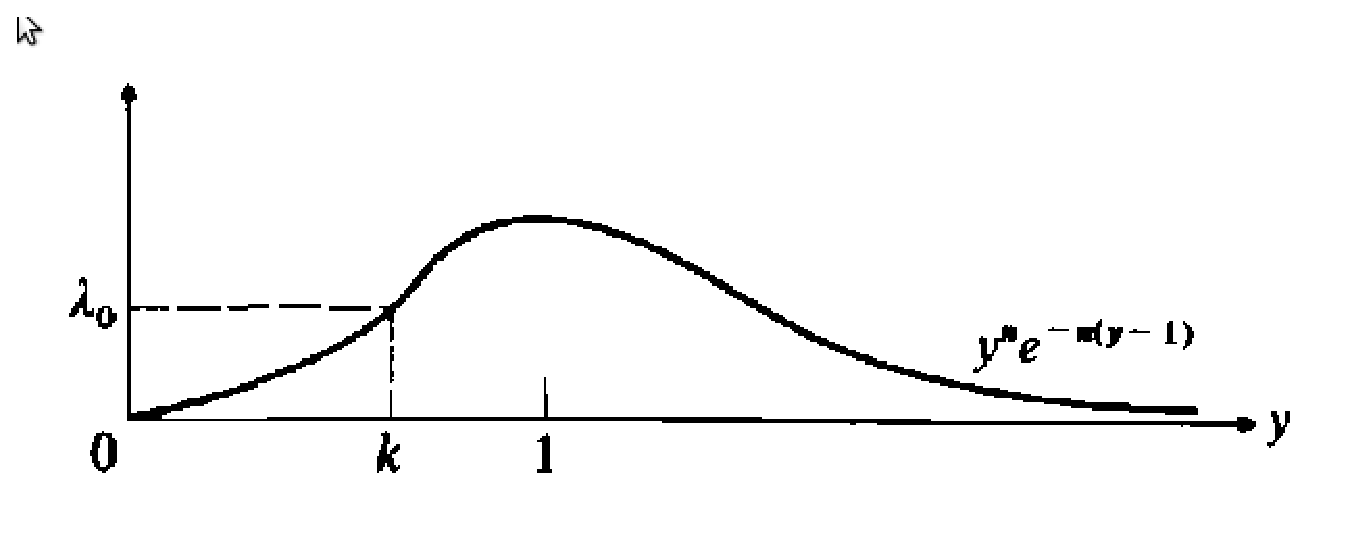
\includegraphics[scale = 0.5]{pictures/example_9_11.eps}
\caption{Funkce charakteristické veličiny}
\label{example_9_11}
\end{figure}

Na závěr uveďme, že vzhledem ke kritériu rozkladu musí obecný věrohodnostní poměrový test záviset pouze na minimální dostatečné statistice.

\subsection{Uniformě nejsilnější test}

\begin{definition}[Uniformě nejsilnější test]
Test $\mathscr{T}^*$ pro $\mathscr{H}_0: \theta \in \overline{\underline{\Theta}}_0$ vs. $\mathscr{H}_1: \theta \in \overline{\underline{\Theta}} - \overline{\underline{\Theta}}_0$ je uniformě nejsilnější test právě tedhy a jen tehdy, jestliže
\begin{enumerate}
\item $\sup_{\theta \in \overline{\underline{\Theta}}_0} \pi_{\mathscr{T}^*}(\theta) = \alpha$\\
\item $\pi_{\mathscr{T}^*}(\theta) \ge \pi_{\mathscr{T}}(\theta)$ pro všechna $\theta \in \overline{\underline{\Theta}} - \overline{\underline{\Theta}}_0$ a libovolný alternativní test $\mathscr{T}$ velikosti menší nebo rovnou $\alpha$.
\end{enumerate}
\end{definition}

Test $\mathscr{T}^*$ je uniformě nejsilnějším testem s velikostí $\alpha$, jestliže mezi všemi ostatními testy s velikostí rovnou nebo menší než $\alpha$ má největší sílu pro všechny alternativní hodnoty $\theta$. Přívlastek ``uniformní'' je váže právě ke ``všem'' alternativním hodnotám $\theta$. Uniformě nejsilnější test pro dané hypotézy nemusí vždy existovat.

\begin{example}
Uvažujme náhodný výběr $X_1, ..., X_n$ z populace $f(x, \theta) = \theta e^{-\theta x}I_{(0, \infty)}(x)$, kde $\overline{\underline{\Theta}} = \{\theta: \theta \ge \theta_0\}$. Pokusme se nalézt uniformě nejsilnější test pro $\mathscr{H}_0: \theta = \theta_0$ vs. $\mathscr{H}_1: \theta > \theta_0$.

Z příkladu (9.7) víme, že pro fixní $\theta_1 > \theta_0$ a   $\mathscr{H}_0: \theta = \theta_0$ vs. $\mathscr{H}_1: \theta = \theta_0$ nejsilnější test zamítne $\mathscr{H}_0$, jestliže $\sum x_i \le k'$, kde $k'$ je dáno řešením rovnice
\begin{equation*}
\alpha = \int_0^{k'} \frac{1}{\Gamma(n)}\theta_0^n x^{n - 1}e^{-\theta_0 x}dx
\end{equation*}
Tento test vyplynul z Neyman-Pearsonovy věty. Vzhledem k tomu, že s vyjímkou podmínky $\theta_1 > \theta_0$ tento test nezávisí na $\theta_1$, zíkali bychom stejný test pro libovolné $\theta_1 > \theta_0$. Proto se jedná o uniformě nejsilnější test.
\end{example}

Následující větu uvádíme bez důkazu.

\begin{theorem}
Uvažujme náhodný výběr $X_1, ..., X_n$ z populace $f(x, \theta)$, kde $\theta \in \overline{\underline{\Theta}}$ a $\overline{\underline{\Theta}}$ je interval. Předpokládejme, že
\begin{equation*}
f(x, \theta) = a(\theta)b(x)e^{c(\theta)d(x)}
\end{equation*}
a definujme statistiku
\begin{equation*}
\mathfrak{t}(x_1, ..., x_n) = \sum_{i = 1}^n d(x_i)
\end{equation*}
\begin{enumerate}
\item Jestliže je $c(\theta)$ monotónní rostoucí funkce v $\theta$ a jestliže existuje $k^*$ takové, že $P_{\theta_0}[\mathfrak{t}(X_1, ..., X_n) > k^*] = \alpha$, pak test $\mathscr{T}^*$ s kritickým regionem $C^* = \{(x_1, ..., x_n): \mathfrak{t}(x_1, ..., x_n) > k^*\}$ je uniformě nejsilnějším testem velikosti $\alpha$ pro $\mathscr{H}_0: \theta \le \theta_0$ vs. $\mathscr{H}_1: \theta > \theta_0$ nebo $\mathscr{H}_0: \theta = \theta_0$ vs. $\mathscr{H}_1: \theta > \theta_0$.
\item Jestliže je $c(\theta)$ monotónní klesající funkce v $\theta$ a jestliže existuje $k^*$ takové, že $P_{\theta_0}[\mathfrak{t}(X_1, ..., X_n) < k^*] = \alpha$, pak test $\mathscr{T}^*$ s kritickým regionem $C^* = \{(x_1, ..., x_n): \mathfrak{t}(x_1, ..., x_n) < k^*\}$ je uniformě nejsilnějším testem velikosti $\alpha$ pro $\mathscr{H}_0: \theta \le \theta_0$ vs. $\mathscr{H}_1: \theta > \theta_0$ nebo $\mathscr{H}_0: \theta = \theta_0$ vs. $\mathscr{H}_1: \theta > \theta_0$.
\end{enumerate}
\end{theorem}

\begin{example}
Uvažujme náhodný výběr $X_1, ..., X_n$ z populace $f(x, \theta) = \theta e^{-\theta x}I_{(0, \infty)}(x)$, kde $\overline{\underline{\Theta}} = \{\theta> \theta > 0\}$. Testované hypotézy mají tvar $\mathscr{H}_0: \theta \le \theta_0$ vs. $\mathscr{H}_1: \theta > \theta_0$. Pravděpodobnostní funkci lze vyjádřit ve tvaru
\begin{equation*}
f(x, \theta) = \theta I_{(0, \infty)}(x)e^{-\theta x} = a(\theta)b(x)e^{c(\theta)d(x)}
\end{equation*}
a proto $\mathfrak{t}(x_1, ..., x_n) = \sum x_i$, $c(\theta) = -\theta$. $c(\theta)$ je monotónní klesající funkce, a proto dle bodu (2) výše uvedené věty uniformě nejsilnější test zamítne $\mathscr{H}_0$ pro $\sum x_i < k^*$, kde $k^*$ je řešením rovnice
\begin{equation*}
\alpha = P_{\theta_0}\left[\sum_{i = 1}^n X_i < k^* \right] = \int_0^{k^*}\frac{1}{\Gamma(n)}\theta_0^n u^{n - 1}e^{-\theta_0 u}du
\end{equation*} 
\end{example}

\begin{definition}[Monotonní věrohodnostní poměr]
O rodině pravděpodobnostních rozdělení $\{f(x, \theta): \theta\ \in \overline{\underline{\Theta}}, \textit{kde} ~ \overline{\underline{\Theta}} ~ \textit{je interval}\}$ říkáme, že mají monotónní věrohodnostní poměr, jestliže existuje statistika $T = \mathfrak{t}(X_1, ..., X_n)$ taková, že poměr
\begin{equation*}
\frac{L(\theta'; x_1, ..., x_n)}{L(\theta''; x_1, ..., x_n)}
\end{equation*}
je buďto nerostoucí funkcí $\mathfrak{t}(x_1, ..., x_n)$ pro každé $\theta' < \theta''$ nebo neklesající funkcí $\mathfrak{t}(x_1, ..., x_n)$ pro každé $\theta' < \theta''$.
\end{definition}

\begin{example}
Jestliže $\{f(x; \theta): \theta \in \overline{\underline{\Theta}}\} = \{\theta e^{-\theta x}I_{(0, \infty)}(x): \theta > 0\}$, pak
\begin{equation*}
\frac{L(\theta'; x_1, ..., x_n)}{L(\theta''; x_1, ..., x_n)} = \frac{(\theta')^n e^{-\theta' \sum_{i = 1}^n x_i}}{(\theta'')^n e^{-\theta'' \sum_{i = 1}^n x_i}} = \left(\frac{\theta'}{\theta''}\right)^n e^{-(\theta' - \theta'')\sum_{i = 1}^n x_i}
\end{equation*}
což je monotónní rostoucí funkce v $\sum x_i$.
\end{example}

\begin{example}
Jestliže $\{f(x; \theta): \theta \in \overline{\underline{\Theta}}\} = \{(1/\theta)I_{(0, \infty)}(x): \theta > 0\}$, pak
\begin{multline*}
\frac{L(\theta'; x_1, ..., x_n)}{L(\theta''; x_1, ..., x_n)} = \frac{\left(\frac{1}{\theta'}\right)^n \prod_{i = 1}^n I_{(0, \theta')}(x_i)}{\left(\frac{1}{\theta''}\right)^n \prod_{i = 1}^n I_{(0, \theta'')}(x_i)}\\
=
\begin{cases}
\left(\frac{\theta''}{\theta'}\right)^n ~ \textit{pro} ~ 0 < y_n < \theta'\\
0 ~ \textit{pro} ~ \theta' \le y_n < \theta''
\end{cases}
\end{multline*}
což je monotónní nerostoucí funkce v $y_n = \max(x_1, ..., x_n)$. Připomeňme, že $y_n$ nemůže padnout mimo interval $(0, \theta'')$, jestliže $\theta$ nabývá hodnoty $\theta'$ nebo $\theta''$.
\end{example}

Následující větu uvádíme bez důkazu.

\begin{theorem}
Uvažujme náhodný výběr $X_1, ..., X_n$ z populace $f(x; \theta)$, kde $\overline{\underline{\Theta}}$ představuje interval. Předpokládejme, že rodina pravděpodobnostních rozdělení $\{f(x;\theta): \theta \in \overline{\underline{\Theta}}\}$ má monotónní věrohodnostní poměr pro statistiku $\mathfrak{t}(X_1, ..., X_n)$.
\begin{enumerate}
\item Jestliže je monotónní věrohodnostní poměr neklesající v $\mathfrak{t}(x_1, ..., x_n)$ a jestliže existuje $k^*$ takové, že $P_{\theta_0}[\mathfrak{t}(X_1, ..., X_n) < k^*] = \alpha$, pak je test odpovídající kritickému regionu $C^* = \{(x_1, ..., x_n): \mathfrak{t}(x_1, ..., x_n) < k^*\}$ uniformě nejsilnější test síly $\alpha$ pro $\mathscr{H}_0: \theta \le \theta_0$ vs. $\mathscr{H}_1: \theta > \theta_0$.
\item Jestliže je monotónní věrohodnostní poměr nerostoucí v $\mathfrak{t}(x_1, ..., x_n)$ a jestliže existuje $k^*$ takové, že $P_{\theta_0}[\mathfrak{t}(X_1, ..., X_n) > k^*] = \alpha$, pak je test odpovídající kritickému regionu $C^* = \{(x_1, ..., x_n): \mathfrak{t}(x_1, ..., x_n) > k^*\}$ uniformě nejsilnější test síly $\alpha$ pro $\mathscr{H}_0: \theta \le \theta_0$ vs. $\mathscr{H}_1: \theta > \theta_0$.
\end{enumerate}
\end{theorem}

\begin{example}
Uvažujme náhodný výběr $X_1, ..., X_n$ z populace $f(x; \theta) = \frac{1}{\theta}I_{(0, \theta)}(x)$, kde $\theta > 0$ a hypotézy $\mathscr{H}_0: \theta \le \theta_0$ vs. $\mathscr{H}_1: \theta > \theta_0$. Z předchozího příkladu víme, že toto pravděpodobnostní rozdělení má monotónní nerostoucí věrohodnostní poměr pro $\mathscr{t}(x_1, ..., x_n) = y_n = \max(x_1, ..., x_n)$. Dle bodu (2) výše uvedené věty je uniformě nejsilnější test velikosti $\alpha$ definován jako zamítnutí $\mathscr{H}_0$, jestliže $y_n > k^*$, kde $k^*$ je řešením rovnice
\begin{equation*}
\alpha = P_{\theta_0}[Y_n > k^*] = \int_{k^*}^{\theta_0}n \left(\frac{y}{\theta_0}\right)^{n - 1} \frac{dy}{\theta_0} = \frac{1}{\theta_0^n}[\theta_0^n - (k^*)^n] = 1 - \left(\frac{k^*}{\theta_0}\right)^n
\end{equation*}
což implikuje $k^* = \theta_0 \sqrt[n]{1 - \alpha}$.
\end{example}

Závěrem uveďme následující tři poznámky. Za prvé, jak ve větě (9.5) tak ve větě (9.6) je nulová hypotéza formulována jako $\theta \le \theta_0$. Jestliže by nulová hypotéza byla formulována jako $\theta \ge \theta_0$, zůstaly by obě věty v platnosti, pokud bychom obrátily nerovnosti, které definují kritický region. Za druhé, věta (9.5) je důsledkem věty (9.6). Za třetí, obě věty uvažují pouze jednostranné hypotézy.

\subsection{Nezkreslený test}

V řadě případů uniformě nejsilnější test neexistuje. V takovém případě můžeme soubor testů omezit a následně nalézt uniformě nejsilnější test na této omezené množině. Tímto se dostáváme ke konceptu nezkresleného testu.

\begin{definition}[Nezkreslený test]
Test $\mathscr{T}$ hypotéz $\mathscr{H}_0: \theta \in \overline{\underline{\Theta}}_0$ vs. $\mathscr{H}_1: \theta \in \overline{\underline{\Theta}}_1$ je nezkreslený test, jestliže
\begin{equation*}
\sup_{\theta \in \overline{\underline{\Theta}}_0} \pi_{\mathscr{T}}(\theta) \le \inf_{\theta \in \overline{\underline{\Theta}}_1}\pi_{\mathscr{T}}(\theta)
\end{equation*}
\end{definition}

V případě nezkresleného testu je tedy pravděpodobnost zamítnutí nepravdivé $\mathscr{H}_0$ přinejmenším stejně velká jako pravděpodobnost zamítnutí pravdivé $\mathscr{H}_0$. Jestliže v rámci takto omezené množiny testů existuje test, který je uniformě nejsilnější, pak se jedná o uniformě nejsilnější nezkreslený test. Pro nalezení uniformě nejsilnějšího nezkresleného testu byla vyvinuta poměrně složitá teorie, která však přesahuje záběr této knihy.

\subsection{Metody pro nalézání testů}

V rámci testu testujeme nulovou hypotézu $\mathscr{H}_0$ proti alternativní hypotéze $\mathscr{H}_1$. Uvažujme stastistiku, která pro obě hypotézy chová ``odlišně'', a pokusme se využít toto odlišné chování pro definici testu. Jako ilustraci uvažujme testování $\mathscr{H}_0: \theta \le \theta_0$ vs. $\mathscr{H}_1: \theta > \theta_1$, kde náhodný výběr $X_1, ..., X_n$ pochází z $f(x; \theta) = \phi_{\theta, 1}(x)$. Statistika $\overline{X}$ sleduje normální rozdělení se střední hodnotou $\theta$ a rozptylem $1/n$. Lze tedy očekávat, že $\overline{X}$ bude menší pro pravdivé $\mathscr{H}_0$ a větší pro pravdivé $\mathscr{H}_1$ - statistika $\overline{X}$ se tak chová odlišně pro nulovou a alternativní hypotézu. Rozumným testem se tedy zdá zamítnutí $\mathscr{H}_0$, je-li $\overline{X} > k$, kde $k$ je dáno velikostí testu\footnote{Z předchozí kapitoly víme, že takovýto test je uniformě nejsilnější.}.

Klíčem této techniky je tedy nalezení statistiky, která vykazuje ``odlišné'' chování pro nulovou a alternativní hypotézu. Jestliže existuje dostatečná statistika, pak se jedná o přirozeného kandidáta. V opačné případě je možné použít vhodnou funkci odhadu\footnote{Např. funkci odhadu založenou na metodě maximální věrohodnosti.}. Ve výše uvedeném případě tuto funkci plní $\overline{X}$, což zároveň dostatečná statistika a funkce odhadu parametru $\theta$ založená na metodě maximální věrohodnosti.

\begin{example}
Uvažujme náhodný výběr $X_1, ..., X_n$ z Poissonova rozdělení se střední hodnotou $\theta$. Testujeme $\mathscr{H}_0: \theta = \theta_0$ vs. $\mathscr{H}_1: \theta \neq \theta_1$. Předpokládejme $n = 10$ a $\theta_1 = 1$.

Víme, že $\overline{X}$ je funkce odhadu pro $\theta$ založená na metodě maximální věrohodnosti. To znamená, že $\overline{X}$ bude mít tendenci se nacházet v okolí $\theta_0$, jestliže je $\mathscr{H}_0$ pravdivá. Přirozená formulace testu tedy zní: ``Přijmi $\mathscr{H}_0$, jestliže $c_1 < \overline{x} < c_2$'', kde $c_1$ a $c_2$ jsou zvoleny tak, aby měl test požadovanou velikost. Např. test ``přijmi $\mathscr{H}_0$, jestliže $0.4 < \overline{x} < 1.6$'' má velikost
\begin{multline*}
1 - P_{\theta = 1}[0.4 < \overline{X} < 1.6] = 1 - P_{\theta = 1}[4 < \sum_{i = 1}^{10} X_i < 16]\\
= 1 - \sum_{j = 5}^{15}\frac{e^{-10}10^j}{j!} \approx 0.078
\end{multline*}
\end{example}

Test, který je běžně používán v praxi, testuje $\mathscr{H}_0: \theta = \theta_0$ vs. $\mathscr{H}_1: \theta \neq \theta_0$. Pro ilustraci předpokládejme, že $\theta$ je rozdílem výnosů dvou odrůd pšenice. Na první pohled by se mohlo zdát, že kandidátem na vhodný test je $\mathscr{H}_0: \theta = 0$ vs. $\mathscr{H}_1: \theta \neq 0$, který testuje, zda-li existuje rozdíl ve výnosech obou odrůd. Nicméně $\theta$ je spojitá veličina, a proto není možné, aby nabývala právě hodnoty nula. Jako vhodnější se proto jeví test $\mathscr{H}_0: \theta_1 le \theta \le \theta_2$ vs. $\mathscr{H}_1: \theta < \theta_1 ~ \textit{nebo} ~ \theta > \theta_2$. Nalézt odpovídající uniformě nejsilnější test může být složité či dokonce nemožné. Nicméně jestliže $f(x; \theta)$ je pravděpodobnostním rozdělením s jedním parametrem, pak lze pro konstrukci testu použít funkci odhadu $\hat{\Theta}$ založenou na metodě maximální věrohodnosti a síla tohoto testu je pak porovnána s ideální funkcí charakteristické veličiny testu velikosti $\alpha$. Pro některá pravděpodobnostní rozdělení lze použít test, který zamítne $\theta_0$, jestliže se $\hat{\theta}$ nenachází v určitém intervalu $(c_1, c_2)$, kde $c_1$ a $c_2$ mohou být vybrána tak, aby platilo
\begin{equation*}
\int_{c_1}^{c_2} f_{\hat{\Theta}}(\hat{\theta}; \theta_1)d \hat{\theta} = \int_{c_1}^{c_2} f_{\hat{\Theta}}(\hat{\theta}; \theta_2)d \hat{\theta} = 1 - \alpha
\end{equation*}
kde $f_{\hat{\Theta}}(\hat{\theta}, \theta)$ je pravděpodnostní funkce $\hat{\Theta}$ pro parametr $\theta$. Odpovídající funkce charakteristické veličiny je pak
\begin{equation*}
\pi(\theta) = 1 - \int_{c_1}^{c_2}f_{\hat{\Theta}}(\hat{\theta}; \theta) d \hat{\theta} ~ \textit{pro} ~ \theta \in \overline{\underline{\Theta}}
\end{equation*}
Tuto funkci charakteristické veličiny je možné porovnat s ideální funkcí charakteristické veličiny a pokud její odchylka nepřesahuje přijatelnou mez, může být příslušný test použit, i když se nejedná o uniformě nejsilnější test.

\begin{example}
Uvažujme náhodný výběr $X_1, ..., X_n$ z populace $\phi_{\theta, 1}(x)$. Testujme $\mathscr{H}_0: 1 \le \theta \le 2$ vs. $\mathscr{H}_1: \theta < 1 ~ \textit{nebo} ~ \theta > 2$.

Víme, že $\overline{X}$ je funkce odhadu pro $\theta$ dle metody maximální věrohodnosti. Tato statistika sleduje normální rozdělení se střední hodnotou $\theta$ a rozptylem $1/n$. Naším cílem je nalézt $c_1$ a $c_2$ takové, aby platilo
\begin{equation*}
1 - \alpha = \int_{c_1}^{c_2} \phi_{1, 1/n}(x)dx = \int_{c_1}^{c_2} \phi_{2, 1/n}(x)dx
\end{equation*}
tj.
\begin{equation*}
\Phi\left(\frac{c_2 - 1}{\sqrt{1/n}}\right) - \Phi\left(\frac{c_1 - 1}{\sqrt{1/n}}\right) = \Phi\left(\frac{c_2 - 2}{\sqrt{1/n}}\right) - \Phi\left(\frac{c_1 - 2}{\sqrt{1/n}}\right) = 1 - \alpha
\end{equation*}
Jak je patrné z obrázku (\ref{example_9_18a}), platí $c_1 = \frac{3}{2} - d$ a $c_2 = \frac{3}{2} + d$, kde $d$ je dáno
\begin{equation*}
\Phi \left(\frac{d + \frac{1}{2}}{\sqrt{1/n}}\right) - \left(\frac{\frac{1}{2} - d}{\sqrt{1/n}}\right) = 1 - \alpha
\end{equation*}
Jestliže, např. $\alpha = 0.05$ a $n = 16$, pak $d \approx 0.911$, $c_1 \approx 0.589$ a $c_2 \approx 2.411$. Funkce charakteristické veličiny je
\begin{equation*}
\pi(\theta) = 1 - P_{\theta}[c_1 < \overline{X} < c_2] = 1 - P_{\theta}[0.589 < \overline{X} < 2.411]
\end{equation*}
a je ilustrována obrázkem  (\ref{example_9_18b}).
\end{example}

\begin{figure}[htp]
\centering
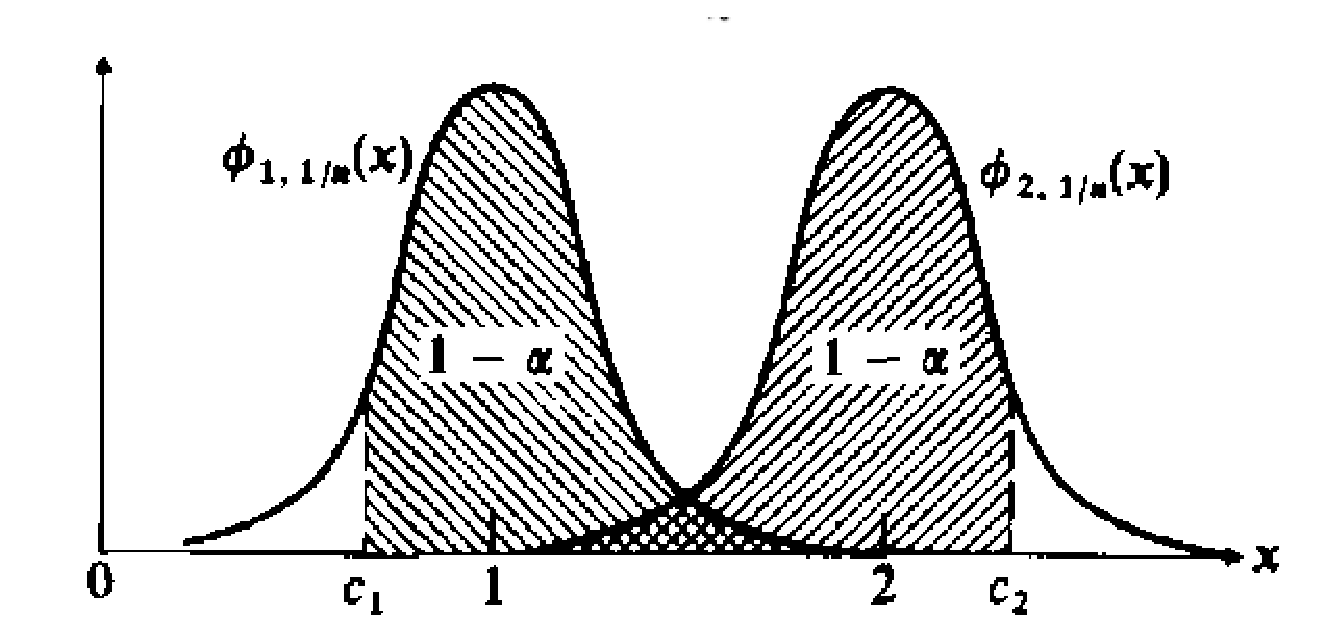
\includegraphics[scale = 0.5]{pictures/example_9_18a.eps}
\caption{Ilustrační obrázek}
\label{example_9_18a}
\end{figure}

\begin{figure}[htp]
\centering
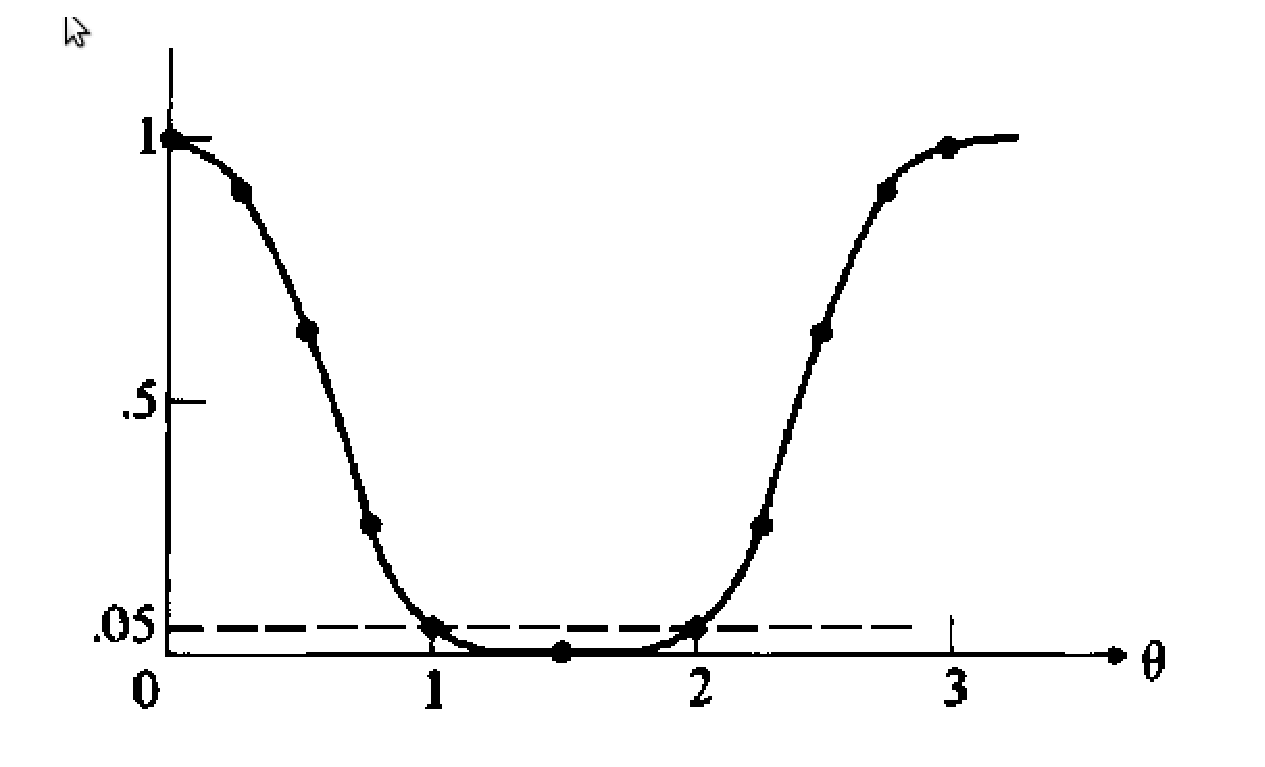
\includegraphics[scale = 0.5]{pictures/example_9_18b.eps}
\caption{Ilustrační obrázek}
\label{example_9_18b}
\end{figure}

\section{Testování hypotéz - výběr z normálního rozdělení}

\subsection{Testování středních hodnot}

\subsubsection{$\mathscr{H}_0: \mu \le \mu_0$ vs. $\mathscr{H}_1: \mu > \mu_0$}

Nejprve předpokládejme, že známe $\sigma^2$. Normální pravděpodobnostní rozdělení
\begin{equation*}
f(x, \theta) = \phi_{\mu, \sigma^2}(x) = \frac{1}{\sqrt{2\pi} \sigma}e^{-\frac{1}{2}\left(\frac{x - \mu}{\sigma}\right)} = \frac{1}{\sqrt{2\pi}\sigma}e^{-\frac{1}{2}\left(\frac{\mu}{\sigma}\right)^2}e^{-\frac{1}{2}\left(\frac{x}{\sigma}\right)^2}e^{\frac{\mu}{\sigma}x}
\end{equation*}
je člen rodiny exponenciálních rozdělení s
\begin{equation*}
a(\mu) = \frac{1}{\sqrt{2 \pi}\sigma}e^{-\frac{1}{2}\left(\frac{\mu}{\sigma}\right)^2}, ~ b(x) = e^{-\frac{1}{2}\left(\frac{x}{\sigma}\right)^2}, ~ c(\mu) = \frac{\mu}{\sigma} ~ a ~ d(x) = x
\end{equation*}
Podmínky věty (9.5) jsou splněny, a proto uniformě nejsilnější test existuje a zavrhuje $\mathscr{H}_0$ pro $\mathfrak{t}(x_1, ..., x_n) = \sum x_i > k^*$, kde $k^*$ je řešením $P_{\mu_0}[\sum X_i > k^*] = \alpha$. Protože $\alpha = P_{\mu_0}[\sum X_i > k^*] = 1 - \Phi\left(\frac{k^* - n \mu_0}{\sqrt{n} \sigma}\right)$, tak $\frac{k^* - n \mu_0}{\sqrt{n} \sigma} = z_{1 - \alpha}$, kde $z_{1 - \alpha}$ je $(1 - \alpha)$-tý kvantil normovaného normálního rozdělení. Test tedy zamítne $\mathscr{H}_0$, jestliže $\sum x_i > n \mu_0 + \sqrt{n}\sigma z_{1 - \alpha}$ neboli $\overline{x} > \mu_0 + \frac{\sigma}{\sqrt{n}}z_{1 - \alpha}$.

Jestliže je $\sigma^2$ neznáme, pak je testování $\mathscr{H}_0: \mu \le \mu_0$ vs. $\mathscr{H}_1: \mu > \mu_0$ ekvivalentní testování $\mathscr{H}_0: \theta \in \overline{\underline{\Theta}}_0$ vs. $\mathscr{H}_1: \theta \notin \mu_0$, kde $\theta = (\mu, \sigma^2)$, $\overline{\underline{\Theta}} = \{(\mu, \sigma^2): -\infty < \mu < \infty; \sigma^2 > 0\}$  a $\overline{\underline{\Theta}}_0 = \{(\mu, \sigma^2): \mu \le \mu_0; \sigma^2 > 0\}$. Pro formulaci testu můžeme (a) použít obecný věrohodnostní poměr nebo (b) nalézt statistiku, která se pro obě hypotézy chová ``odlišně'' a založit na ní test. Příkladem takovéto statistiky je $T = \frac{\overline{X} - \mu_0}{S / \sqrt{n}}$, kde $\overline{X}$ je střední hodnota výběru a $S^2$ je výběrový rozptyl. Protože $T$ bude větší pro $\mu > \mu_0$ než pro $\mu \le \mu_0$, bude test zavrhovat $\mathscr{H}_0$ pro vysoké hodnoty $T$, tj. zamítne $\mathscr{H}_0$, jestliže $T > k$. Jestliže $\mu = \mu_0$, pak $T$ sleduje studentovo rozdělení s $n - 1$ stupni volnosti. $k$ je tak možné získat z $\alpha = P_{\mu_0}[T > k]$, což implikuje $k = t_{1 - \alpha}(n-1)$, tj. $k$ je rovno kvantilu $(1 - \alpha)$ studentova rozdělení s $(n - 1)$ stupni volnosti. Lze dokázat, že takto odvozený test je zároveň testem velikosti $\alpha$ založeným na obecném věrohodnostním poměru.

\subsubsection{$\mathscr{H}_0: \mu = \mu_0$ vs. $\mathscr{H}_1: \mu \neq \mu_0$}

Jestliže známe $\sigma^2$, pak je $\left(\overline{X} - z_{(1 + \gamma)/2}(\sigma / \sqrt{n}), \overline{X} + z_{(1 + \gamma)/2}(\sigma / \sqrt{n})\right)$ je 100$\gamma$ procentní interval spolehlivosti pro $\mu$, kde $z_{(1 + \gamma)/2}$ je $(1 + \gamma)/2$ procentní kvantil normovaného normálního rozdělení. Test pak zamítne $\mathscr{H}_0$, jestliže tento interval nezahrnuje $\mu_0$. Takto definovaný test má navíc velikost $1 - \gamma$, protože
\begin{equation*}
P_{\mu = \mu_0}\left[\overline{X} - z_{(1 + \gamma)/2}\frac{\sigma}{\sqrt{n}} < \mu_0 < \overline{X} + z_{(1 + \gamma)/ 2} \frac{\sigma}{\sqrt{n}}\right] = \gamma
\end{equation*}

Jestliže je $\sigma^2$ neznámé, pak lze odvodit test podobný výše uvedenému, který vychází z 100$\gamma$ procentního intervalu spolehlivosti
\begin{equation*}
\left(\overline{X} - t_{(1 + \gamma)/2}(n - 1)\frac{S}{\sqrt{n}}, \overline{X} + t_{(1 + \gamma)/2}(n - 1) \frac{S}{\sqrt{n}}\right)
\end{equation*}
Pokusme se však nalézt test založený na obecném věrohodnostním poměru. Funkce maximální věrohodnosti má tvar
\begin{equation*}
L(\mu, \sigma^2; x_1, ..., x_n) = \left(\frac{1}{\sqrt{2 \pi} \sigma}\right)^n e^{-\frac{1}{2}\sum_{i = 1}^n \left(\frac{x_i - \mu}{\sigma}\right)^2}
\end{equation*}
$\overline{\underline{\Theta}}_0 = \{(\mu, \sigma^2): \mu = \mu_0; \sigma^2 > 0\}$ a $\overline{\underline{\Theta}} = \{(\mu, \sigma^2): -\infty < \mu < \infty; \sigma^2 > 0\}$. Víme, že hodnoty pro $\mu$ a $\sigma^2$, které maximalizují $L(\mu, \sigma^2; x_1, ..., x_n)$ nad $\overline{\underline{\Theta}}$, jsou $\hat{\mu} = \overline{x}$ a $\hat{\sigma}^2 = \frac{\sum_{i = 1}^n (x_i - \overline{x})^2}{n}$, proto
\begin{equation*}
\sup_{\overline{\underline{\Theta}}} L(\mu, \sigma^2; x_1, ..., x_n) = \left(\frac{n}{2 \pi \sum_{i = 1}^n (x_i - \overline{x})^2}\right)^{n/2}e^{-n/2}
\end{equation*}
Abychom maximalizovali $L(\mu, \sigma^2; x_1, ..., x_n)$ nad $\overline{\underline{\Theta}}_0$, dosaďme $\mu = \mu_0$. Jediným neznámým parametrem tak zůstává $\sigma^2$, který maximalizuje $L(\mu, \sigma^2; x_1, ..., x_n)$ pro $\frac{\sum (x_i - \mu_0)^2}{n}$, čímž získáváme
\begin{equation*}
\sup_{\overline{\underline{\Theta}}_0} L(\mu, \sigma^2; x_1, ..., x_n) = \left(\frac{n}{2 \pi \sum_{i = 1}^n (x_i - \mu_0)^2}\right)^{n/2}e^{-n/2}
\end{equation*}
Obecný věrohodností poměr je tak
\begin{gather*}
\lambda = \left(\frac{\sum_{i = 1}^n (x_i - \overline{x})^2}{\sum_{i = 1}^n (x_i - \mu_0)^2}\right)^{n/2} = \left(\frac{\sum_{i = 1}^n (x_i - \overline{x})^2}{\sum_{i = 1}^n (x_i - \overline{x} + \overline{x} + \mu_0)^2}\right)^{n/2}\\
\left(\frac{\sum_{i = 1}^n (x_i - \overline{x})^2}{\sum_{i = 1}^n (x_i - \overline{x})^2 + n(\overline{x} - \mu)^2}\right)^{n/2} = \left(\frac{1}{1 + n(\overline{x} - \mu_0)^2 / \sum_{i = 1}^n(x_i - \overline{x})^2}\right)^{n/2}
\end{gather*}
Všimněme si, že $\lambda$ je monotónní funkcí pro statistiku
\begin{equation*}
t^2 = \mathfrak{t}^2(x_1, ..., x_n) - \frac{n(n - 1)(\overline{x} - \mu_0)^2}{\sum_{i = 1}^n (x_i - \overline{x})^2} = \left(\frac{\overline{x} - \mu_0}{\sqrt{\sum_{i = 1}^n (x_i - \overline{x})^2 / (n-1)n}}\right)^2
\end{equation*}
a proto je kritický region ve tvaru $\lambda \le \lambda_0$ ekvivalentní kritickému regionu ve tvaru $\mathfrak{t}^2(x_1, ..., x_n) \ge k^2$. Test založený obecném věrohodnostním poměru tak zamítne $\mathscr{H}_0$, jestliže
\begin{equation*}
T^2 = \left(\frac{\overline{X} - \mu_0}{S / \sqrt{n}}\right)^2 \ge k^2
\end{equation*}
neboli přijme $\mathscr{H}_0$, jestliže $-k < T < k$. Protože $T$ sleduje studentovo rozdělení s $n - 1$ stupni volnosti pro $\mu = \mu_0$, je $k$ vybráno tak, aby splňovalo
\begin{equation*}
\int_{-k}^k f_T(t; n-1)dt = 1 - \alpha
\end{equation*}
kde $\alpha$ je požadovaná velikost testu. To znamená, že $k$ je rovno $t_{(1 - \alpha)/2}(n - 1)$, tj. kvantilu $(1 - \alpha)/2$ studentova rozdělení s $n - 1$ stupni volnosti. Takto odvozený test se shoduje s testem založeném na intervalu spolehlivosti, který jsme definovali na začátku jako
\begin{equation*}
\left(\overline{X} - t_{(1 + \gamma) / 2}(n - 1)\frac{S}{\sqrt{n}}, \overline{X} + t_{(1 + \gamma)/2}(n - 1)\frac{S}{\sqrt{n}}\right)
\end{equation*}
kde $\gamma = 1 - \alpha$. Bez důkazu uveďme, že tento test je také uniformě nejsilnějším testem.

\subsubsection{Ostatní případy}

Ve výše uvedeném textu jsme odvodili test střední hodnoty normálního rozdělení pro jednostrané i oboustranné hypotézy. Jednostrannou nulovou hypotézu $\mu \le \mu_0$ lze obrátit a získat příslušný test. Je možné definovat také další typy hypotéz, jako např. $\mathscr{H}_0: \mu_1 \le \mu \le \mu_2$ vs. $\mathscr{H}_1: \mu < \mu_1 ~ \textit{nebo} ~ \mu > \mu_2$.

\subsection{Testování rozptylu}

\subsubsection{$\mathscr{H}_0: \sigma^2 \le \sigma_0^2$ vs. $\sigma^2 > \sigma_0^2$}

Předpokládejme, že $\mu$ je známo. Pak je parametrický prostor reprezentovaný intervalem. Námi uvažovaný test je jednostranný, a proto máme naději nalézt uniformě nejsilnější test velikosti $\alpha$. Pravděpodobnostní funkce normálního rozdělení
\begin{equation*}
f(x; \theta) = f(x; \sigma^2) = \frac{1}{\sqrt{2 \pi} \sigma}e^{-\frac{1}{2 \sigma^2}(x - \mu)^2}
\end{equation*}
je člen rodiny exponenciálních rozdělení s $a(\sigma^2) = \frac{1}{\sqrt{2 \pi} \sigma}$, $b(x) = 1$, $c(\sigma^2) = -\frac{1}{2}\sigma^2$ a $d(x) = (x - \mu)^2$. $c(\sigma^2)$ je monotónní rostoucí funkce v $\sigma^2$, a proto dle věty (9.5) je test s kritickým regionem $\{(x_1, ..., x_n): \sum (x_i - \mu)^2 > k^*\}$ uniformě nejsilnějším testem velikosti $\alpha$, přičemž $k^*$ je dáno rovnicí $P_{\sigma^2 = \sigma_0^2}[\sum (X_i - \mu)^2 > k^*] = \alpha$. To implikuje $k^* = \sigma_0^2 \chi_{1 - \alpha}^2(n)$, kde $\chi_{1 - \alpha}^2(n)$ je $1 - \alpha$ procentní kvantil chi-kvadrát rozdělení s $n$ stupni volnosti.

Jestliže $\mu$ není známé, lze test odvodit s pomocí statistiky $V = \frac{\sum(X_i - \overline{X})}{\sigma_0^2}$. Statistika $V$ bude nabývat vysokých hodnot pro $\sigma^2 > \sigma_0^2$, a proto test bude zamítat $\mathscr{H}_0$ pro vysoká $V$. Jestliže $\sigma^2 = \sigma_0^2$, pak bude $V$ sledovat chi-kvadrát rozdělení s $n - 1$ stupni volnosti a $P_{\sigma^2 = \sigma_0^2}[V > \chi_{1 - \alpha}^2(n - 1)] = \alpha$, kde $\chi_{1 - \alpha}^2(n - 1)$ je $(1 - \alpha)$ procentní kvantil chi-kvadrát rozdělení s $n - 1$ stupni volnosti. Lze dokázat, že test, který zamítne $\mathscr{H}_0$ pro $\frac{(X_i - \overline{X})^2}{\sigma_0^2} > \chi_{1 - \alpha}^2(n - 1)$, je také testem velikosti $\alpha$ založeným na obecném věrohodnostním poměru.

\subsubsection{$\mathscr{H}_0: \sigma^2 = \sigma_0^2$ vs. $\sigma^2 \neq \sigma_0^2$}

Vynechme situaci, kdy je $\mu$ známo a zaměřme se na situaci, kdy $\mu$ neznáme. V tomto případě je $\overline{\underline{\Theta}}_0 = \{(\mu, \sigma): - \infty < \mu < \infty; \sigma^2 = \sigma_0^2 \}$. Pokusme se nalézt test velikosti $\alpha$ s využitím metody intervalu spolehlivosti. Z kapitoly (8.2.2) víme, že 100$\gamma$ procentní interval spolehlivosti pro $\sigma^2$ je definován jako
\begin{equation*}
\left(\frac{(n - 1)S^2}{q_2}, \frac{(n - 1)S^2}{q_1}\right)
\end{equation*}
kde $q_1$ a $q_2$ jsou kvantily chi-kvadrát rozdělení $f_Q(q; n - 1)$ s $n - 1$ stupni volnosti, kde
\begin{equation*}
\int_{q_1}^{q_2} f_Q(q; n - 1)dq = \gamma
\end{equation*}
Test velikosti $\alpha = 1 - \gamma$ pak přijme $\mathscr{H}_0$, jestliže $\sigma_0^2$ je obsaženo ve výše uvedeném intervalu. Lze dokázat, že tento test odpovídá testu založeném na obecném věrohodnostním poměru.

\subsection{Test několika středních hodnot}

\subsubsection{Test dvou středních hodnot}

Uvažujme dvě vzájemně nezávislé populace, které sledují normální rozdělení - jednu se střední hodnotou $\mu_1$ a rozptylem $\sigma_1^2$ a druhou se střední hodnotou $\mu_2$ a rozptylem $\sigma_2^2$. Testujme hypotézy $\mathscr{H}_0: \mu_1 = \mu_2, \sigma_1^2 > 0, \sigma_2^2 > 0$ vs. $\mathscr{H}_1: \mu_1 \neq \mu_2, \sigma_1^2 > 0, \sigma_2^2 > 0$. Parametrický prostor $\overline{\underline{\Theta}}$ je tedy čtyřrozměrný a příslušné sdružené pravděpodobnostní rozdělení je definováno skrze $(\mu_1, \mu_2, \sigma_1^2, \sigma_2^2)$. Podprostor $\overline{\underline{H}}_0$ je pak pouze třírozměrný, protože $\mu_1 = \mu_2 = \mu$. Uvažujme náhodný výběr $X_{11}, ..., X_{1n_1}$ z první a náhodný výběr  $X_{21}, ..., X_{2n_2}$ z druhé populace. Funkce věrohodnosti je pak definována jako
\begin{multline*}
L(\mu_1, \mu_2, \sigma_1^2, \sigma_2^2; x_{11}, ..., x_{1n_1}, x_{21}, ..., x_{2n_2}) = L\\
= \left(\frac{1}{2\pi \sigma_1^2}\right)^{n_1/2}e^{-\frac{1}{2}\sum_{i = 1}^n \left(\frac{x_{1i} - \mu_1}{\sigma_1}\right)^2} \left(\frac{1}{2\pi \sigma_2^2}\right)^{n_2/2}e^{-\frac{1}{2}\sum_{j = 1}^n \left(\frac{x_{2j} - \mu_2}{\sigma_2}\right)^2}
\end{multline*}
a její maximum nad $\overline{\underline{\Theta}}$ je
\begin{equation*}
\sup_{\overline{\underline{\Theta}}}L = \left(\frac{n_1}{2 \pi \sum_{i = 1}^{n_1}(x_{1i} - \overline{x}_1)^2}\right)^{n_1/2} \left(\frac{n_2}{2 \pi \sum_{j = 1}^{n_2}(x_{2j} - \overline{x}_2)^2}\right)^{n_2/2}e^{-n_1/2}e^{-n_2/2}
\end{equation*}
Jestliže použijeme $\mu_1 = \mu_2 = \mu$ a pokusíme se maximalizovat $L$ vzhledem k $\mu, \sigma_1^2$ a $\sigma_2^2$, zjistíme, že odhad $\mu$ má charakter kořene polynomu třetího řádu a že se jedná o poměrně složitou funkci. To znamená, že také obecný věrohodnostní poměr $\lambda$ je složitou funkcí, která navíc obsahuje podíl rozptylů $\sigma_1^2$ a $\sigma_2^2$ a její pravděpodobnostní funkce je velmi náročná na odvození. Je tedy nemožné analyticky odvodit kritický region $0 < \lambda < k$ pro danou pravděpodobnost chyby typu I, protože poměr rozptylů uvažovaných populací není znám. Kořen polynomu třetího řádu je možné vypočíst numericky, což nám následně umožní výpočet $\lambda$. Pro velké populace navíc, jak si ukážeme v kapitole (9.5), platí, že $- \ln(\Lambda)$ přibližně sleduje chi-kvadrát rozdělení s jedním stupněm volnosti. To nám umožní konstrukci testu, který zamítne $\mathscr{H}_0$ pro velká $-2 \ln(\lambda)$.

Jestliže mají obě uvažované populace shodný rozptyl, problematika se značně zjednoduší. Parametrický prostor $\overline{\underline{\Theta}}$ se stává třírozměrným se souřadnicemi $(\mu_1, \mu_2, \sigma^2)$ a parametrický prostor $\overline{\underline{\Theta}}_0$ dvourozměrným se souřadnicemi $(\mu, \sigma^2)$. Pro $\overline{\underline{\Theta}}$ jsou odhady pro $\mu_1, \mu_2$ a $\sigma^2$ dány $\overline{x}_1$, $\overline{x}_2$ a $\frac{1}{n_1 + n_2}\left(\sum_{i = 1}^{n_1}(x_{1i} - \overline{x}_1)^2 + \sum_{i = 1}^{n_2}(x_{2j} - \overline{x}_2)^2\right)$, a proto
\begin{equation*}
\sup_{\overline{\underline{\Theta}}}L = \left(\frac{n_1 + n_2}{2 \pi \left(\sum_{i = 1}^{n_1} (x_{1i} - \overline{x}_1)^2 + \sum_{j = 1}^{n_2}(x_{2j} - \overline{x}_2)^2\right)}\right)^{(n_1 + n_2)/2}e^{-(n_1 + n_2)/2}
\end{equation*}
Pro $\overline{\underline{\Theta}}_0$ jsou odhady pro $\mu$ a $\sigma^2$ založené na metodě maximální věrohodnosti dány
\begin{equation*}
\hat{\mu} = \frac{1}{n_1 + n_2}\left(\sum_{i = 1}^{n_1} x_{1i} + \sum_{j = 1}^{n_2} x_{2j} \right) = \frac{n_1 \overline{x}_1 + n_2 \overline{x}_2}{n_1 + n_2}
\end{equation*}
a
\begin{multline*}
\hat{\sigma}^2 = \frac{1}{n_1 + n_2}\left(\sum_{i = 1}^{n_1}(x_{1i} - \hat{\mu})^2 + \sum_{j = 1}^{n_2}(x_{2j} - \hat{\mu})^2 \right)\\
= \frac{1}{n_1 + n_2}\left(\sum_{i = 1}^{n_1} (x_{1i} - \overline{x}_1)^2 + \sum_{j = 1}^{n_2}(x_{2j} - \overline{x}_2)^2 + \frac{n_1 n_2}{n_1 + n_2}(\overline{x}_1 - \overline{x}_2)^2\right)
\end{multline*}
čímž získáme
\begin{equation*}
\sup_{\overline{\underline{\Theta}}_0} L = \left(\frac{n_1 + n_2}{2 \pi \left(\sum_{i = 1}^{n_1}(x_{1i} - \overline{x}_1)^2 + \sum_{j = 1}^{n_2}(x_{2j} - \overline{x}_2)^2 + \frac{n_1n_2}{n_1 + n_2}(\overline{x}_1 - \overline{x}_2)^2\right)}\right)^\frac{n_1 + n_2}{2} e^{-\frac{n_1 + n_2}{2}}
\end{equation*}
Obecný věrohodnostní poměr je tak roven
\begin{equation*}
\lambda = \left(1 + \frac{\frac{n_1n_2}{n_1 + n_2}(\overline{x}_1 - \overline{x}_2)^2}{\sum_{i = 1}^{n_1}(x_{1i} - \overline{x}_1)^2 + \sum_{j = 1}^{n_2}(x_{2j} - \overline{x}_2)^2} \right)^{-\frac{n_1 + n_2}{2}}
\end{equation*}
Tento výraz je velmi podobný tomu, který jsme odvodili v kapitole (9.4.1). Příslušný test se pak také opírá o studentovo rozdělení. Víme, že $\overline{X}_1$ a $\overline{X}_2$ jsou nezávislé náhodné veličiny, které sledují normální rozdělení se střední hodnotou $\mu_1$ resp. $\mu_2$ a rozptylem $\sigma^2/n$ a $\sigma^2/n_2$. Je zřejmé, že $\overline{X}_1 - \overline{X}_2$ je normálně rozdělené se střední hodnotou $\mu_1 - \mu_2$ a rozptylem $\sigma^2\left(\frac{1}{n_1} + \frac{1}{n_2}\right)$. Pro nulovou hypotézu je střední hodnota $\overline{X}_1 - \overline{X}_2$ rovna 0. $\frac{\sum(X_{1i} - \overline{X}_1)^2}{\sigma^2}$ a  $\frac{\sum(X_{2j} - \overline{X}_2)^2}{\sigma^2}$ jsou nezávislé a sledují chi-kvadrát rozdělení s $n_1 - 1$ resp. $n_2 - 1$ stupni volnosti. Jeji součet tedy také sleduje chi-kvadrát rozdělení s $n_1 + n_2 - 2$ stupni volnosti. Protože pro nulovou hypotézu sleduje $Z = \frac{\overline{X}_1 - \overline{X}_2}{\sigma \sqrt{1/n_1 + 1/n_2}}$ normální rozdělení s nulovou střední hodnotou a jednotkovým rozptylem, sleduje
\begin{equation*}
T = \frac{\sqrt{\frac{n_1 n_2}{n_1 + n_2}}(\overline{X}_1 - \overline{X}_2)}{\sqrt{\frac{\sum_{i = 1}^{n_1}(X_{1i} - \overline{X}_1)^2 + \sum_{j = 1}^{n_2}(X_{2j} - \overline{X}_2)^2}{n_1 + n_2 - 2}}}
\end{equation*}
studentovo rozdělení s $n_1 + n_2 - 2$ stupni volnosti\footnote{Ve výše uvedené rovnici jsou čitatel a jmenovatel vzájemně nezávislí.}. Obecný věrohodnostní poměr  je pak
\begin{equation*}
\lambda = \left(\frac{1}{1 + \frac{t^2}{n_1 + n_2 - 2}}\right)^{\frac{n_1 + n_2}{2}}
\end{equation*}
a sleduje studentovo rozdělení. Např. 5 procentní kritický region pro $T$ je $T^2 > [t_{0.975}(n_1 + n_2 - 2)]^2$, kde $t_{0.975}(n_1 + n_2 - 2)$ je 0.975 procentní kvantil studentova rozdělení s $n_1 + n_2 - 2$ stupni volnosti.

Pokud bychom chtěli testovat $\mathscr{H}_0: \mu_1 = \mu_2$ vs. $\mathscr{H}_1: \mu_1 > \mu_2$ nebo $\mathscr{H}_0: \mu_1 \le \mu_2$ vs. $\mathscr{H}_1: \mu_1 > \mu_2$, pak by test s velikostí $\alpha$ zamítl $\mathscr{H}_0$ jestliže $T > t_{1 - \alpha}(n_1 + n_2 - 2)$.

\subsubsection{Test několika středních hodnot}

Výše uvedený test lze rozšířit ze dvou na $k$ normálních rozdělení. Uvažujme náhodný výběr $X_{j1}, ...., X_{jn_j}$ z $j$-té populace se střední hodnotou $\mu_j$ a rozptylem $\sigma^2$. Předpokládejme, že všech $k$ populací je vzájemně nezávislých. Testujme nulovou hypotézu, že střední hodnoty všech $k$ populací jsou shodné proti alternativní hypotéze, že tomu tak není. Pro konstrukci testu použijme obecný věrohodnostní poměr.

Funkce maximální věrohodnosti má tvar
\begin{multline*}
L(\mu_1, ..., \mu_k, \sigma^2; x_{11}, ..., x_{1n_1}, ..., x_{k1}, ..., x_{kn_k})\\
= \prod_{j = 1}^k \prod_{i = 1}^{n_j} \frac{1}{\sqrt{2 \pi} \sigma}e^{-\frac{1}{2}\left(\frac{(x_{ji} - \mu_j)}{\sigma}\right)^2} = \left(\frac{1}{\sqrt{2 \pi} \sigma}\right)^n e^{-\frac{1}{2 \sigma^2}\sum_{j = 1}^k \sum_{i = 1}^{n_j}(x_{ji} - \mu_j)^2}
\end{multline*}
kde $n = \sum_{j = 1}^k n_j$. Parametrický prostor $\overline{\underline{\Theta}}$ je $(k+1)$-rozměrný prostor se souřadnicemi $(\mu_1, ..., \mu_k, \sigma^2)$ a $\overline{\underline{\Theta}}_0$ je dvourozměrným parametrickým prostorem se souřadnicemi $\mu, \sigma^2$, kde $\mu = \mu_1 = ... = \mu_k$. Pro $\overline{\underline{\Theta}}$ jsou odhady pro $\mu_1, ..., \mu_k, \sigma^2$ založené na metodě maximální věrohodnosti definovány jako
\begin{equation*}
\hat{\mu}_j = \overline{x}_{j \cdot} = \frac{1}{n_j} \sum_{i = 1}^{n_j}x_{ji}, ~~~ j = 1, ..., k
\end{equation*}
a
\begin{equation*}
\hat{\sigma}_{\overline{\underline{\Theta}}}^2 = \frac{1}{n}\sum_{j = 1}^k \sum_{i = 1}^{n_j}(x_{ji} - \overline{x}_{j \cdot})^2
\end{equation*}
a proto
\begin{equation*}
\sup_{\overline{\underline{\Theta}}}L = \left(\frac{2 \pi \sum_{j = 1}^k \sum_{i = 1}^{n_j} (x_{ji} - \overline{x}_{j\cdot})^2}{n}\right)^{-\frac{n}{2}}e^{-\frac{n}{2}}
\end{equation*}
Pro $\overline{\underline{\Theta}}_0$ jsou ohady pro $\mu$ a $\sigma^2$ založené na metodě maximální věrohodnosti definovány jako
\begin{equation*}
\hat{\mu} = \overline{x} = \frac{1}{n}\sum_{j = 1}^k \sum_{i = 1}^{n_j}x_{ji}
\end{equation*}
a
\begin{equation*}
\hat{\sigma}_{\overline{\underline{\Theta}}_0^2} = \frac{1}{n}\sum_{j = 1}^k \sum_{i = 1}^{n_j}(x_{ji} - \overline{x})^2
\end{equation*}
a proto
\begin{equation*}
\sup_{\overline{\underline{\Theta}}_0} L = \left(\frac{2 \pi \sum_{j = 1}^k \sum_{i = 1}^{n_j}(x_{ji} - \overline{x})^2}{n}\right)^{-\frac{n}{2}}e^{-\frac{n}{2}}
\end{equation*}
Obecný věrohodnostní poměr je pak definován jako
\begin{multline*}
\lambda = \frac{\sup_{\overline{\underline{\Theta}}_0} L}{\sup_{\overline{\underline{\Theta}}}} = \left(\frac{\sum_{j = 1}^k \sum_{i = 1}^{n_k}(x_{ji} - \overline{x})^2}{\sum_{j = 1}^k \sum_{i = 1}^{n_j}(x_{ji} - \overline{x}_{j \cdot})^2}\right)^{-\frac{n}{2}}\\
= \left(\frac{\sum_{j = 1}^k \sum_{i = 1}^{n_j}(x_{ji} - \overline{x}_{j \cdot} + \overline{x}_{j \cdot} - \overline{x}_{j \cdot} - \overline{x})^2}{\sum_{j = 1}^k \sum_{i = 1}^{n_1} (x_{ji} - \overline{j \cdot})^2}\right)^{-\frac{n}{2}}
= \left(\frac{\sum_{j = 1}^k \sum_{i = 1}^{n_j}(x_{ji} - \overline{x}_{j \cdot})^2 + \sum_{j = 1}^k n_j (\overline{x}_{j \cdot} - \overline{x})^2}{\sum_{j = 1}^k \sum_{i = 1}^{n_1} (x_{ji} - \overline{j \cdot})^2}\right)^{-\frac{n}{2}}\\
= \left(1 + \frac{k - 1}{n - k}\frac{\sum_{j = 1}^k n_j(\overline{x}_{j \cdot} - \overline{x})^2/(k - 1)}{\sum_{j = 1}^k \sum_{i = 1}^{n_j}(x_{ji} - \overline{x}_{j \cdot})^2 / (n - k)}\right)^{-\frac{n}{2}}
\end{multline*}
Test založený na obecném věrohodnostním poměru zamítne $\mathscr{H}_0$, jestliže $\lambda \le \lambda_0$. Nicméně $\lambda \le \lambda_0$ pouze jestliže
\begin{equation*}
r = \frac{\sum_{j = 1}^k n_j (\overline{x}_{j \cdot} - \overline{x})^2 / (k - 1)}{\sum_{j = 1}^k \sum_{i = 1}^{n_j}(x_{ji} - \overline{x}_{j \cdot}) / (n - k)} \ge c
\end{equation*}
kde $c$ je konstanta. Poměr $r$ nazýváme rozptylovým poměr nebo také $F$ poměrem. Konstanta $c$ je zvolena tak, aby $P[R \ge c | \mathscr{H}_0]$. Vzhledem k tomu, že $\overline{X}_{j \cdot}$ a $\sum_{i = 1}^{n_j}(X_{ji} - \overline{X}_{j \cdot})^2$ jsou vzájemně nezávislé, proto jsou také čitatel a jmenovatel v $r$ nezávislí. Pro hypotézu $\mathscr{H}_0$ sleduje čitatel vydělený $\sigma^2$ chi-kvadrát rozdělení s $k - 1$ stupni volnosti a jmenovatel vydělený $\sigma^2$ pak chi-kvadrát rozdělení s $n - k$ stupni volnosti. Je-li tedy $\mathscr{H}_0$ pravdivé, sleduje $R$ rozdělení $F$ s $k - 1$ a $n - k$ stupni volnosti a konstanta $c$ tak představuje $(1 - \alpha)$ procentní kvantil $F$ rozdělení s  $k - 1$ a $n - k$ stupni volnosti.

Výše popsaný způsob testování se nazývá analýza rozptylu. Smysl tohoto pojmu je patrný, jestliže si uvědomíme, že jmenovatel $r$ je odhadem rozptylu v rámci jednotlivých populací a čitatel je odhadem rozptylu mezi populacemi za předpokladu shodné střední hodnoty. Při testování středních hodnot tak paradoxně tak analyzujeme rozptyl.

\subsection{Testování několika rozptylů}

\subsubsection{Testování dvou rozptylů}

Uvažujme náhodné výběry ze dvou populací, které sledují normální rozdělení s parametry $(\mu_1, \sigma_1^2)$ a $\mu_2, \sigma_2^2$. V následujícím textu budeme uvažovat následující hypotézy
\begin{enumerate}
\item $\mathscr{H}_0: \sigma_1^2 \le \sigma_2^2$ vs. $\mathscr{H}_1: \sigma_1^2 > \sigma_2^2$
\item $\mathscr{H}_0: \sigma_1^2 \ge \sigma_2^2$ vs. $\mathscr{H}_1: \sigma_1^2 < \sigma_2^2$
\item $\mathscr{H}_0: \sigma_1^2 = \sigma_2^2$ vs. $\mathscr{H}_1: \sigma_1^2 \neq \sigma_2^2$
\end{enumerate}
Uvažujme náhodný výběr  $X_{11}, ..., X_{1n_1}$ z normálního rozdělení se střední hodnotou $\mu_1$ a rozptylem $\sigma_1^2$ a náhodný výběr  $X_{21}, ..., X_{2n_2}$ z normálního rozdělení se střední hodnotou $\mu_2$ a rozptylem $\sigma_2^2$. Předpokládejme nezávislost těchto dvou náhodných výběrů. Víme, že poměr
\begin{equation*}
\frac{\sum_{i = 1}^{n_1}(X_{1i} - \overline{X}_1)/(n_1 - 1)\sigma_1^2}{\sum_{i}^{n_2}(X_{2i} - \overline{X}_2)/(n_2 - 1)\sigma_2^2}
\end{equation*}
sleduje $F$ rozdělení s $n_1 - 1$ a $n_2 - 1$ stupni volnosti a konkrétně statistika
\begin{equation*}
R = \frac{(n_2 - 1)\sum_{i = 1}^{n_1}(X_{1i} - \overline{X}_1)^2}{(n_1 - 1)\sum_{i = 1}^{n_2}(X_{2i} - \overline{X}_2)^2}
\end{equation*}
sleduje $F$ rozdělení s $n_1 - 1$ a $n_2 - 1$ stupni volnosti pro $\sigma_1^2 = \sigma_2^2$. Statistika $R$ bude nabývat větších hodnot pro $\sigma_1^2 > \sigma_2^2$ a menších hodnot pro $\sigma_1^2 < \sigma_2^2$, čehož lze využít při formulaci testu. Např. test $\mathscr{H}_0: \sigma_1^2 \le \sigma_2^2$ vs. $\mathscr{H}_1: \sigma_1^2 > \sigma_2^2$ zamítne $\mathscr{H}_0$, jestliže $R$ přesáhne $F_{\alpha}(n_1 - 1, n_2 - 1)$, tj. $\alpha$ procentní kvantil $F$ rozdělení s $n_1 - 1$ a $n_2 - 1$ stupni volnosti. Test $\mathscr{H}_0: \sigma_1^2 = \sigma_2^2$ vs. $\mathscr{H}_1: \sigma_1^2 \neq \sigma_2^2$ přijme $\mathscr{H}_0$, jestliže $k_1 < R < k_2$, kde $k_1$ a $k_2$ jsou vybrány tak, aby test měl velikost $\alpha$. Běžně se volí $k_1 = F_{\alpha/2}(n_1 - 1, n_2 - 1)$ a $k_2 =  F_{1 - \alpha/2}(n_1 - 1, n_2 - 1)$, tj. oba chvosty mají plochu $\alpha/2$, ačkoliv se nejedná o nejlepší možný test.

Na závěr uveďme, že ke stejným výsledků bychom dospěli také s pomocí obecného věrohodnostního poměru.

\subsubsection{Testování rovnosti několika rozptylů}

Uvažujme náhodný výběr $X_{j1}, ..., X_{jn_j}$ z populace, která sleduje normální rozdělení se střední hodnotou $\mu_j$ a rozptylem $\sigma_j^2$, kde $j = 1, ..., k$. Předpokládejme, že jednotlivé výběry jsou vzájemně nezávislé. Testujme nulovou hypotézu $\mathscr{H}_0: \sigma_1^2 = \sigma_2^2 = \cdots = \sigma_k^2$ proti alternativní hypotéze $\mathscr{H}_1$, že rozptyly jednotlivých náhodných výběrů nejsou shodné.

Funkce maximální věrohodnosti je
\begin{equation*}
L(\mu_1, ..., \mu_k, \sigma_1^2, ..., \sigma_k^2; x_{11}, ..., x_{1n_1}, ..., x_{k1}, ..., x_{k n_k}) = \prod_{j = 1}^k \prod_{i = 1}^{n_j}\frac{1}{\sqrt{2 \pi}\sigma_j}e^{-\frac{1}{2}\left(\frac{x_{ji} - \mu_j}{\sigma_j}\right)^2}
\end{equation*}
a odhady pro $\mu_j$, $\sigma_j^2$ založené na metodě maximální věrohodnosti jsou
\begin{equation*}
\hat{\mu}_j = \frac{1}{n_j}\sum_{i = 1}^{n_j} x_{ji} = \overline{x}_{j \cdot}
\end{equation*}
a
\begin{equation*}
\hat{\sigma}_j^2 = \frac{1}{n_j}\sum_{i = 1}^{n_j}(x_{ji} - \overline{x}_{j \cdot})^2
\end{equation*}
Dle nulové hypotézy jsou všechny rozptyly shodné, tj. $\sigma^2 = \sigma_1^2, ..., \sigma_k^2$. Parametrický prostor $\overline{\underline{\Theta}}_0$ je tedy definován jako $\{(\mu_1, ..., \mu_k, \sigma^2): -\infty < \mu_j < \infty; \sigma^2 > 0\}$ a odhady pro $\mu_1, ..., mu_k, \sigma^2$ dle metody maximální věrohodnosti nad $\overline{\underline{\Theta}}_0$ jsou
\begin{equation*}
\hat{\mu}_j = \overline{x}_j
\end{equation*}
a
\begin{equation*}
\hat{\sigma}^2 = \frac{1}{\sum_{j = 1}^k n_j} \sum_{j = 1}^k \sum_{i = 1}^{n_j} (x_{ji} - \overline{x}_{j \cdot})^2 = \frac{\sum_{j = 1}^k n_j \hat{\sigma}_j^2}{\sum_{j = 1}^n n_j}
\end{equation*}
Proto
\begin{multline*}
\lambda = \frac{\sup_{\overline{\underline{\Theta}}_0}L}{\sup_{\overline{\underline{\Theta}}}L} = \frac{\left(\frac{1}{\hat{\sigma}^2}\right)^{\sum_{j = 1}^k n_j/k}e^{-\sum_{j = 1}^k n_j/2}}{\prod_{j = 1}^k \left(\frac{1}{\hat{\sigma}_j^2}\right)^{n_j/2} e^{-\sum_{j = 1}^k n_j/2}}\\
= \frac{\prod_{j = 1}^k(\hat{\sigma}_j^2)^{n_j/2}}{\left(\sum_{j = 1}^k n_j \hat{\sigma}_j^2 / \sum_{j = 1}^k\right)^{\sum_{j = 1}^k n_j/2}}
\end{multline*}
Test zamítne $\mathscr{H}_0$, jestliže $\lambda \le \lambda_0$. Nalezení konkrétní hodnoty $\lambda_0$, která by odpovídala testu velikosti $\alpha$, je však problematické, protože pravděpodobnostní rozdělení statistiky $\Lambda$ nelze analyticky vyjádřit. Avšak, stejně jako v předchozím textu, lze tento problém obejít v případě výběrů dostatečně velkého rozsahu, proto které $-2 \ln(\Lambda)$ přibližně sleduje chi-kvadrát rozdělení s $k - 1$ stupni volnosti. Výše popsaný test tak zamítne $\mathscr{H_0}$, jestliže $-2 \ln(\lambda) > \chi_{1 - \alpha}(k - 1)$, kde $\chi_{1 - \alpha}(k - 1)$ představuje $1 - \alpha$ procentní kvantil chi-kvadrát rozdělení s $k - 1$ stupni volnosti.

\section{Chi-kvadrát testy}

V následujícím textu představíme testy, které jsou postaveny na chi-kvadrát rozdělení. Soustředíme se pouze na nalezení testu pro určitou hypotézu bez ohledu na otázku jejich optimality, a proto se nebudeme zabývat funkcí charakteristické veličiny.

\subsection{Asymptotické rozdělení obecného věrohodnostního poměru}

V předchozím textu jsme dvakrát konstatovali, že pravděpodobnostní rozdělení obecného věrohodnostního poměru je složité odvodit, nicméně že existuje asymptotické rozdělení, které lze použít pro jeho aproximaci. Následující věta, kterou však nebudeme dokazovat, nám dává toto asymptotické rozdělení.

\begin{theorem}
Uvažujme náhodný výběr $X_1, ..., X_n$ se sdruženou pravděpodobnostní funkcí $f_{X_1, ..., X_n}(\cdot, ..., \cdot; \theta)$, kde $\theta = (\theta_1, ..., \theta_k)$ splňuje podmínky regularity. Předpokládejme, že parametrický prostor $\overline{\underline{\Theta}}$ je $k$ rozměrný. Pro hypotézu
\begin{equation*}
\mathscr{H}_0: \theta_1 = \theta_1^0, ..., \theta_r = \theta_r^0, \theta_{r + 1}, ..., \theta_k
\end{equation*}
kde $\theta_1^0, ..., \theta_r^0$ jsou známé a $\theta_{r + 1}, ..., \theta_k$ nejsou specifikovány, sleduje $-2 \ln(\Lambda_n)$ pro pravdivé $\mathscr{H}_0$ přibližně chi-kvadrát rozdělení s $r$ stupni volnosti za předpokladu dostatečně velkého náhodného výběru.
\end{theorem}

Ve výše uvedené větě jsme předpokládali, že $1 \le r \le k$. Jestliže $r = k$, jsou všechny parametry specifikovány. Parametrický prostor $\overline{\underline{\Theta}}$ je $k$ rozměrný, a protože $\mathscr{H}_0$ specifikuje $r$ parametrů, je parametrický prostor $\overline{\underline{\Theta}}_0$ $k - r$ rozměrný. Připomeňme, že $\Lambda_n$ je náhodná veličina, která má hodnotu
\begin{equation*}
\lambda_n = \frac{\sup_{\overline{\underline{\Theta}}_0}L(\theta_1, ..., \theta_k; x_1, ..., x_n)}{\sup_{\overline{\underline{\Theta}}}L(\theta_1, ..., \theta_k; x_1, ..., x_n)}
\end{equation*}
což je obecný věrohodnostní poměr náhodného výběru velikosti $n$. $\overline{\underline{\Theta}}$ je podmnožinou $\overline{\underline{\Theta}}$ specifikovanou skrze hypotézu $\mathscr{H}_0$. V případě testu založeného na obecném věrohodnostním poměru zamítáme hypotézu $\mathscr{H}_0$ pro malá $\lambda_n$. Nicméně protože $-2 \ln(\lambda_n)$ roste s klesajícím $\lambda_n$, zamítáme $\mathscr{H}_0$ pro vysoké hodnoty $-2 \ln(\lambda_n)$. Odpovídající test o přibližné\footnote{Připomeňme, že se jedná o aproximaci.} síle $\alpha$ tedy zamítá $\mathscr{H}_0$, jestliže $-2 \ln(\lambda_n) > \chi_{1 - \alpha}^2(r)$, kde $\chi_{1 - \alpha}^2(r)$ představuje $(1 - \alpha)$ procentní kvantil chi-kvadrát rozdělení s $r$ stupni volnosti.

Vzhledem ke tvaru nulové hypotézy by se mohlo zdát, že výše uvedená věta má pouze omezené použití. Nicméně, jak ilustruje níže uvedené příklady, lze někdy upravit pravděpodobnostní rozdělení tak, aby bylo možné formulovat nulovou hypotézu v požadovaném tvaru.

\begin{example}
V kapitole (9.4.3) jsme testovali střední hodnoty dvou normálních rozdělení pomocí hypotéz $\mathscr{H}_0: \mu_1 = \mu_2, \sigma_1^2 > 0, \sigma_2^2 > 0$ vs. $\mathscr{H}_1: \mu_1 \neq \mu_2, \sigma_1^2 > 0, \sigma_2^2 > 0$. Parametrický prostor je čtyř rozměrný a ačkoliv se nulová hypotéza $\mathscr{H}_0$ na první pohled nezdá být v požadovaném tvaru, lze ji snadno upravit. Nechť $\theta_1 = \mu_1 - \mu_2, \theta_2 = \mu_2, \theta_3 = \sigma_1^2$ a $\theta_4 = \sigma_2^2$. Nulová hypotéza tak přejde do tvaru $\mathscr{H}_0: \theta_1 = \theta_1^0 = 0, \theta_2, \theta_3, \theta_4$, tj. první parametr je roven nule a zbývající tři nejsou specifikovány. To znamená, že je-li $\mathscr{H}_0$ pravdivé, pak $-2 \ln(\Theta')$ sleduje chi-kvadrát rozdělení s jedním stupněm volnosti, kde $\Theta'$ je statistika, která představuje obecný věrohodnostní poměr pro pozměněnou $\mathscr{H}_0$. Nicméně vzhledem k invarianci funkcí odhadu založených na metodě maximální věrohodnosti je $\Theta'$ stejné jako $\Theta$ pro původní formulaci $\mathscr{H}_0$.
\end{example}

\begin{example}
V kapitole (9.4.4) jsme testovali $\mathscr{H}_0: \sigma_1^2 = \cdots = \sigma_m^2, \mu_1, ..., \mu_m$. Nulovou hypotézu $\mathscr{H}_0$ lze upravit pomocí substitucí
\begin{equation*}
\theta_1 = \frac{\sigma_1^2}{\sigma_m^2}, ..., \theta_{m - 1} = \frac{\sigma_{m - 1}^2}{\sigma_m^2}, \theta_m = \sigma_m^2, \theta_{m + 1} = \mu_1, ..., \theta_{m + m} = \mu_m
\end{equation*}
do tvaru
\begin{equation*}
\mathscr{H}_0: \theta_1 = 1, ..., \theta_{m - 1} = 1, \theta_m, \theta_{m + 1}, ..., \theta_{2m}
\end{equation*}
tj. prvních $m - 1$ parametrů je rovno jedné a zbylé parametry nejsou specifikovány. Stejně jako v předchozím případě i zde jsou obecné věrohodnostní poměry před a po transformaci shodné a statistika $-2 \ln(\Theta)$, je-li $\mathscr{H}_0$ pravdivé, sleduje chi-kvadrát rozdělení s $m - 1$ stupni volnosti.
\end{example}

\subsection{Chi-kvadrat test dobré shody}

Uvažujme populaci, která sleduje multinomiální pravděpodobnostní rozdělení
\begin{equation*}
f(x_1, ..., x_k; p_1, ..., p_k) = \prod_{j = 1}^{k + 1}p_j^{x_j}
\end{equation*}
kde $j = 1, ..., k + 1$, $x_j$ nabývá hodnot 0 nebo 1, $0 \le p_j \le 1, \sum x_j = 1$ a $\sum p_j = 1$. Jedná se tedy o stejnou situaci, jakou je výběr s vracením z populace, jejíž prvky mohou být rozděleny do $k + 1$ skupin. Klasickým předmětem testování je, zda-li pravděpodobnost $p_j$ odpovídá konkrétní hodnotě\footnote{Pokud bycho házeli hrací kostkou, mohli bychom se ptát, zda-li je tato kostka správně vyvážená, tj. zda-li $p_j = \frac{1}{6}$ pro $j = 1, ..., 6$.}. Výsledek jednoho experimentu lze popsat pomocí náhodných veličin $(X_1, ..., X_k)$, kde $X_j = 1$ jestliže výsledek experimentu odpovídá skupině $j$, jinak $X_j = 0$. Výsledek $n$ pokusů tak lze popsat jako
\begin{equation*}
(X_{11}, ..., X_{1k}), (X_{21}, ..., X_{2k}), ..., (X_{n1}, ..., X_{nk})
\end{equation*}
Definujme $N_j = \sum_{i = 1}^n X_{ij}$, tj. $N_j$ představuje počet experimentů, jejichž výsledky odpovídaly kategorii $j$. Z kapitoly (4.1.2) víme, že náhodná veličina $(N_1, ..., N_k)$ sleduje multinomiální rozdělení.

Pro testování nulové hypotézy $\mathscr{H}_0: p_j = p_j^0, j = 1, ..., k + 1$, kde $p_j^0$ představují známé pravděpodobnosti a jejichž součet je roven jedné, použijeme obecný věrohodnostní moment. Funkce maximální věrohodnosti je rovna
\begin{equation*}
L = L(p_1, ..., p_k; x_{11}, ..., x_{1k}, ..., x_{n1}, ..., x_{nk}) = \prod_{i = 1}^n \prod_{j = 1}^{k + 1} p_j^{x_{ij}}
\end{equation*}
Parametrický prostor $\overline{\underline{\Theta}}$ je $k$ rozměrný\footnote{Parametrů $p_j$ je sice $k + 1$, avšak jeden rozměr ``ubírá'' podmínka $\sum p_j = 1$.}, zatímco parametrický prostor $\overline{\underline{\Theta}}$ je jednorozměrný. Lze snadno dokázat, že $L$ je nad $\overline{\underline{\Theta}}$ maximalizováno pro
\begin{equation*}
p_j = \sum_{i = 1}^n \frac{x_{ij}}{n} = \frac{n_j}{n}
\end{equation*}
kde $n_j$ je hodnota náhodné veličiny $N_j$. Proto
\begin{equation*}
\sup_{\overline{\underline{\Theta}}} L = \frac{1}{n^n}\prod_{j = 1}^{k + 1}n_j^{n_j}
\end{equation*}
Maximum $L$ nad $\overline{\underline{\Theta}}_0$ je rovno $\prod_{j = 1}^{k + 1} (p_j^0)^{n_j}$ a obecný věrohodnostní poměr je tak roven
\begin{equation*}
\lambda = n^n \prod_{j = 1}^{k + 1}\prod_{j = 1}^{k + 1}\left(\frac{p_j^0}{n_j}\right)^{n_j}
\end{equation*}
Nulová hypotéza $\mathscr{H}_0$ je tak zamítnuta, jestliže $\lambda < \lambda_0$, kde $\lambda$ je konstanta zvolená s ohledem na požadovanou velikost chyby typu I. Pro dostatečně velká $n$ lze použít aproximaci pomocí $-2 \ln(\Lambda)$, které sleduje chi-kvadrát rozdělení s $k$ stupni volnosti. Tato aproximace je překvapivě dobrá také pro malá $n$ za předpokladu, že $k > 0$.

Další test, který se běžně používá pro testování $\mathscr{H}_0$, byl navržen Karlem Pearsonem ještě před obecnou teorií testování hypotéz. Tento test se opírá o statistiku
\begin{equation*}
Q_k^0 = \sum_{j = 1}^{k + 1}\frac{(N_j - np_j^0)^2}{np_j^0}
\end{equation*}
která je malá pro pravdivou $\mathscr{H}_0$ malá a velká pro nepravdivou $\mathscr{H}_0$. $N_j$ představuje pozorovaný počet experimentů, jejichž realizace odpovídala skupině $j$ a $np_j^0$ pak představuje očekávaný počet realizací za předpokladu pravdivosti $\mathscr{H}_0$. Lze snadno dokázat, že
\begin{equation*}
E[Q_k^0] = \sum_{j = 1}^{k + 1}\frac{1}{np_j^0}[np_j(1 - p_j) + n^2(p_j - p_j^0)^2]
\end{equation*}
kde $p_j$ představuje skutečnou hodnotu parameteru. Jestliže je $\mathscr{H}_0$ pravdivé, pak $E[Q_k^0] = \sum (1 - p_j^0) = k + 1 - 1 = k$. Následující věta uvádí limitující pravděpodobnostní rozdělení pro $Q_k^0$ za předpokladu pravdivosti $\mathscr{H}_0$.

\begin{theorem}
Předpokládejme, že možné výsledky určitého experimentu je možné rozdělit do $k + 1$ vzájemně neslučitelných skupin $A_1, ..., A_{k + 1}$. Definujme $p_j = P[A_j]$, kde $j = 1, ..., k + 1$. Nechť v rámci $n$ náhodných experimentů představuje $N_j$ počet realizací, které odpovídají skupině $A_j$. Platí tedy $\sum_{j = 1}^{k + 1}N_j = n$. Pak náhodná veličina $\frac{(N_j - n p_j)^2}{np_j}$ sleduje pravděpodobnostní rozdělení, které se s rostoucím $n$ limitně blíží chi-kvadrát rozdělení s $k$ stupni volnosti.
\end{theorem}

\begin{proof}
Výše uvedenou větu nedokážeme v její obecné podobě, ale pouze pro $k = 1$. Potřebujeme dokázat, že pro každé $x$ konverguje $F_{Q_k(x)}$ k $F_{\chi^2(k)}(x)$ s tím, jak se $n$ blíží k nekonečnu. $F_{Q_k}(\cdot)$ představuje kumulativní distribuční funkci náhodné veličiny $Q_k$ a $F_{\chi^2(k)}(\cdot)$ představuje kumulativní distribuční funkci chi-kvadrát rozdělení s $k$ stupni volnosti. Pro $k = 1$ platí
\begin{multline*}
Q_k = Q_1 = \frac{(N_1 - np_1)^2}{np_1} + \frac{(N_2 - np_2)^2}{np_2}\\
= \frac{(N_1 - np_1)^2}{np_1} + \frac{(n - N_1 - n + np_1)^2}{n(1 - p_1)}\\
= \frac{(N_1 - np_1)^2}{np_1(1 - p_1)}
\end{multline*}
Víme, že $N_1$ sleduje binomické rozdělení s parametry $n$ a $p_1$ a že $Y_n = \frac{N_1 - np_1}{\sqrt{np_1(1 - p_1)}}$ tudíž limitně sleduje normované normální rozdělení. Protože druhá mocnina normované normální veličiny sleduje  chi-kvadrát rozdělenení, a protože $Y_n^2 = Q_1$, sleduje také $Q_1$ chi-kvadrát rozdělení.
\end{proof}

Výše uvedená věta nám poskytuje limitní rozdělení pro statistiku
\begin{equation*}
Q_k^0 = \sum_{j = 1}^{k + 1}\frac{(N_j - np_j^0)^2}{np_j^0}
\end{equation*}
za předpokladu pravdivosti nulové hypotézy $\mathscr{H}_0: p_j = p_j^0, j = 1, ..., k + 1$. Test s přibližnou velikostí $\alpha$ tak zamítne $\mathscr{H}_0$, jestliže $Q_k^0 > \chi_{1 - \alpha}^2(k)$.

Ve výše uvedeném textu jsme uvedli věty (9.7) a (9.8) s jejichž pomocí lze testovat shodnou hypotézu $\mathscr{H}_0$. Ačkoliv jsou odpovídající testy na první pohled rozdílné, lze dokázat, že jsou, v případě náhodného výběru velkého rozsahu, ekvivalentní.

\begin{example}
Při svých pokusech přírodopisec Gregor Mendel zjistil, že kuličky hrášku lze rozdělit do čtyř skupin podle barvy a tvaru a to konkrétně na (a) žlutý a kulatý, (b) zelený a kulatý, (c) žlutý a hranatý a (d) zelený a hranatý a to přibližně v poměru 9/3/3/1. Pro $n = 556$ kuliček hrášku jsme zjistily
\begin{center}
  \begin{tabular}{|l|r|r|}
    \hline
    \textbf{Typ} & \textbf{pozorovaný počet} & \textbf{očekávaný počet}\\
    \hline
    žlutý a kulatý & 315 & 312.75\\
    zelený a kulatý & 108 & 104.25\\
    žlutý a hranatý & 101 & 104.25\\
    zelený a kulatý & 32 & 34.75\\
    \hline
  \end{tabular}
\end{center}
Test velikosti $\alpha$ zamítne nulovou hypotézu $\mathscr{H}_0: p_1 = \frac{9}{16}, p_2 = \frac{3}{16}, p_3 = \frac{3}{16}, p_4 = \frac{1}{16}$, jestliže
\begin{equation*}
Q_3^0 = \sum_{j = 1}^4 \frac{(N_j - n p_j^0)^2}{n p_j^0} > \chi_{1 - \alpha}^2(k) = \chi_{0.95}^2(3) = 7.81
\end{equation*}
Pozorované $Q_3^0$ má hodnotu
\begin{equation*}
\frac{(315 - 312.75)^2}{312.75} + \frac{(108 - 104.25)^2}{104.25} + \frac{(101 - 104.25)^2}{104.25} + \frac{(32 - 34.75)^2}{34.75} \approx 0.470
\end{equation*}
a proto můžeme konstatovat dobrou shodu mezi modelem a skutečnými pozorováními.
\end{example}

Následující věta, jejíž důkaz však přesahuje záběr knihy, je zobecněním věty (9.8) pro případ, kdy pravděpodobnosti $p_1$ závisí na neznámém parametru.

\begin{theorem}
Uvažujme náhodný experiment, jehož realizace lze rozdělit do $k + 1$ vzájemně neslučitelných skupin $A_1, ..., A_{k + 1}$. Definujme $p_j = P[A_j], j = 1, ..., k + 1$ a předpokládejme, že $p_j$ závisí na $r$ neznámých parametrech $\theta_1, ..., \theta_r$, tj. $p_j = \mathfrak{p}_j(\theta_1, ..., \theta_r), j = 1, ..., k + 1$. Nechť pro $n$ vzájemně nezávislých pokusů představuje $N_j$ počet realizací, které náleží do skupiny $A_j, j = 1, ..., k + 1$, přičemž $\sum N_j = n$. Dále nechť $\hat{\Theta}_1, ..., \hat{\Theta}_r$ jsou BAN funkce odhadu\footnote{Např. funkce odhadu založené na metodě maximální věrohodnosti.} pro $\theta_1, ..., \theta_r$, které jsou založené na $N_1, ..., N_k$. Pak, jestliže $\mathfrak{p}_j$ splňují podmínky regularity, limitně sleduje
\begin{equation*}
Q'_k = \sum_{j = 1}^{k + 1}\frac{(N_j - n \hat{P}_j)^2}{n \hat{P}_j}
\end{equation*}
chi-kvadrát rozdělení s $k - r$ stupni volnosti, kde $\hat{P}_j = \mathfrak{p}_j(\hat{\Theta}_1, ..., \hat{\Theta}_r), j = 1, ..., k + 1$.
\end{theorem}

Výše uvedená věta neobsahuje žádnou explicitní zmínku o testování hypotéz. V následujícím textu si ukážeme, jak lze závěry této věty použít pro formulaci testu dobré shody. Předpokládejme, že potřebujeme otestovat, zda-li náhodný výběr $X_1, ..., X_n$ pochází z populace $f(x; \theta_1, ..., \theta_r)$, kde parametry $\theta_1, ..., \theta_r$ jsou neznámé, avšak funkční předpis $f$ známe. Nulová hypotéza má charakter složené hypotézy $\mathscr{H}_0: X_i ~ \textit{má pravděpodobnostní funkci} ~ f(x; \theta_1, ..., \theta_r) ~ \textit{pro daná} ~ \theta_1, ..., \theta_r$. Nulová hypotéza tedy tvrdí, že náhodný výběr pochází z populace $f(\cdot; \theta_1, ..., \theta_r)$. Dále předpokládejme, že hodnoty, kterých může náhodná veličina $X_i$ nabývat, jsou rozděleny na $k + 1$ vzájemně neslučitelných skupin $A_1, ..., A_{k + 1}$, že $p_j = P[X_i \in A_j]$ a že $N_j$ je počet $X_i$ náležících do $A_j$. Za předpokladu pravdivosti $\mathscr{H}_0$ a pro dostatečně velké $n$ pak z věty (9.9) vyplývá, že náhodná veličina 
\begin{equation*}
Q'_k = \sum_{j = 1}^{k + 1} \frac{(N_j - n \hat{P}_j)^2}{n \hat{P}_j}
\end{equation*}
přibližně sleduje chi-kvadrát rozdělení s $k - r$ stupni volnosti, kde $\hat{P}_j = \mathfrak{p}_j(\hat{\Theta}_1, ..., \hat{\Theta}_r)$ a $\hat{\Theta}_i$ je funkce odhadu dle metody maximální věrohodnosti pro $\theta_i, i = 1, ..., r$, která je založená na statistikách $N_1, ..., N_k$\footnote{Připomeňme, že $\mathfrak{p}_j(\theta_1, ..., \theta_r) = P[X_i \in A_j]$, což je v případě spojité náhodné veličiny $X_i$ rovno $\int_{A_j}f(x; \theta_1, ..., \theta_r)dx$.}. Test tak zamítne $\mathscr{H}_0$ pro $Q'_k > \chi^2_{1 - \alpha}(k - r)$, kde $\chi^2_{1 - \alpha}(k - r)$ je $1 - \alpha$ procentní kvantil chi-kvadrát rozdělení s $k - r$ stupni volnosti. Tento test nazýváme testem dobré shody, protože testuje, zda-li jsou pozorování konzistentní s předpokladem, že pocházejí z pravděpodobnostního rozdělení $f(x; \theta_1, ..., \theta_r)$, tj. že se s tímto pravděpodobnostním rozdělením shodují.

Parametry $\theta_1, ..., \theta_r$ jsme namísto pozorování $X_1, ..., X_n$ odhadli pomocí statistik $N_1, .., N_k$. Tyto parametry je však možné odhadnout také pomocí funkce odhadu dle metody maximální věrohodnosti s využitím $X_1, ..., X_n$. Limitní pravděpodobnostní rozdělení náhodné veličiny $Q_k'$ tak již nesleduje chi-kvadrát rozdělení s $k - r$ stupni volnost, ale je ohraničena chi-kvadrát rozdělením s $k - r$ stupni volnosti a chi-kvadrát rozdělením s $k$ stupni volnosti.

\begin{example}
Uvažujme náhodný výběr $X_1, ..., X_n$. Testujme, zda-li tento náhodný výběr pochází z normálního rozdělení.

Rozděleme pozorování $x_1, ..., x_n$ do $k + 1$ skupin, kde $j$-tá skupina představuje všech pozorování, která spadají do intervalu $(z_{j - 1}, z_j], j = 1, ..., k + 1$ pro $z_0 < z_1 < \cdots < z_k < z_{k + 1}$, kde $z_0 = \infty$ a $z_{k + 1} = \infty$. Pak platí
\begin{equation*}
p_j = \mathfrak{p}_j(\mu, \sigma^2) = \int_{z_{j - 1}^{z_j}}\phi_{\mu, \sigma^2}(x)dx = \Phi\left(\frac{z_j - \mu}{\sigma}\right) - \Phi\left(\frac{z_{j - 1} - \mu}{\sigma}\right)
\end{equation*}
Nechť jsou $\hat{\mu}$ a $\hat{\sigma}$ odhady dle metody maximální věrohodnosti založené na $n_1, ..., n_k$, kde $n_j$ představuje počet pozorování v $j$-tém intervalu. Pak lze
\begin{equation*}
\hat{p}_j  = \Phi\left(\frac{z_j - \hat{\mu}}{\hat{\sigma}}\right) - \Phi \left(\frac{z_{j-1} - \hat{\mu}}{\hat{\sigma}}\right)
\end{equation*}
vypočíst na základě pozorování stejně jako hodnota
\begin{equation*}
q'_k = \sum_{j = 1}^{k + 1} \frac{(n_j - n \hat{p}_j)^2}{n \hat{p}_j}
\end{equation*}
náhodné veličiny $Q'_k$. Nulová hypotéza, že vzorek pochází z normálního rozdělení bychom na hladině $\alpha$ zamítly, jestliže $q'_k > \chi^2_{1 - \alpha}(k - 2)$.

Jestliže bychom $\mu$ a $\sigma$ odhadli dle metody maximální věrohodnosti na základě $x_1, ..., x_n$, pak by asymptotické rozdělení náhodné veličiny $Q'_k$ bylo ohraničeno chi-kvadrát rozdělením s $k - 2$ stupni volnosti a chi-kvadrát rozdělením s $k$ stupni volnosti. Nulovou hypotézu bychom tedy zamítli, jestliže $q'_k > C$, kde $C$ se nachází mezi $\chi^2_{1 - \alpha}(k - 2)$ a $\chi_{1 - \alpha}^2(k)$. Na závěr dodejme, že pro velké $k$ je rozdíl mezi $\chi^2_{1 - \alpha}(k - 2)$ a $\chi_{1 - \alpha}^2(k)$ zanedbatelný.
\end{example}

\subsection{Test shodnosti dvou multinomiálních rozdělení}

Uvažujme dvě multinomiální rozdělení, jejichž realizace možné rozdělit do $k + 1$ skupin. Nechť jsou pravděpodobnosti odpovídající prvnímu z rozdělení $p_{11}, ..., p_{1k}, p_{1,k+1}$ a pravděpodobnosti odpovídající druhému rozdělení pak $p_{21}, ..., p_{2k}, p_{2,k+1}$. Nulová hypotéza má tvar $\mathscr{H}_0: p_{1j} = p_{2j} = p_j$ pro $j = 1, ..., k + 1$. Předpokládejme, že první náhodný výběr má velikost $n_1$ a druhý náhodný výběr pak velikost $n_2$. Definujme $N_{1j}$ jako počet realizací v $j$-té skupině prvního výběru a $N_{2j}$ jako počet realizací v $j$-té skupině druhého výběru, kde $j = 1, ..., k + 1$. Víme, že statistika
\begin{equation*}
\sum_{j = 1}^{k + 1} \frac{(N_{ij} - n_i p_{ij})^2}{n_i p_{ij}}
\end{equation*}
limitně sleduje chi-kvadrát rozdělení s $k$ stupni volnosti pro $i = 1, 2$. Proto, jsou-li náhodné výběry vzájemně nezávislé a $\mathscr{H}_0$ pravdivá, sleduje
\begin{equation*}
Q_{2k}\sum_{i = 1}^2 \sum_{j = 1}^{k + 1} \frac{(N_{ij} - n_i p_{ij})^2}{n_i p_{ij}}
\end{equation*}
limitně chi-kvadrát rozdělení $2k$ stupni volnosti. Jestliže $\mathscr{H}_0$ specifikuje hodnotu $p_j$, pak je $Q_{2k}$ statistikou a její hodnotu lze použít přímo při konstrukci testu. Jestliže však $\mathscr{H}_0$ hodnotu $p_j$ nespecifikuje, pak musí být $p_j$ odhadnuto. Jestliže je $\mathscr{H}_0$ pravdivá, pak lze oba náhodné výběry považovat za jeden náhodný výběr z multinomiálního rozdělení s pravděpodobnostmi $p_1, ..., p_{k + 1}$. Funkce odhadu dle metody maximální věrohodnosti je $p_j = \frac{N_{1j} + N_{2j}}{n_1 + n_2}, j = 1, ..., k + 1$, čímž získáme
\begin{equation*}
Q_{2k}' = \sum_{i = 1}^2 \sum_{j = 1}^{k + 1} \frac{\left(\frac{N_{ij} - n_i(N_{1j} + N_{2j})}{n_1 + n_2}\right)^2}{\frac{n_i(N_{1j} + N_{2j})}{n_1 + n_2}}
\end{equation*}
Lze dokázat, že $Q'_{2k}$ limitně sleduje chi-kvadrát rozdělení s $2k - k = k$ stupni volnosti\footnote{Počet stupňů volnosti limitního pravděpodobnostního rozdělení pro $Q'_{2k}$ byl snížen o jedna pro každý odhadovaný parametr.}.

Alternativní test shody dvou multinomiálních rozdělení lze odvodit pomocí obecného věrohodnostního poměru $\Lambda$ s využitím věty (9.7) a limitního rozdělení $-2 \ln(\Lambda)$.

\begin{example}
Předpokládejme, že provádíme výzkum veřejného mínění a zajímá nás, zda-li voliči pod 25 let zastávají odlišné názory než voliči nad 25 let. Dále předpokládejme, že bylo osloveno 1000 voličů do 25 let a 1500 voličů nad 25 let a že jejich odpovědi na jednu konkrétní otázku shrnuje následující tabulka.
\begin{center}
  \begin{tabular}{|c|c|c|c|c|}
    \hline
    \textbf{skupina} & \textbf{proti} & \textbf{neví} & \textbf{pro} & \textbf{celkem}\\
    \hline
    pod 25 let & 400 & 100 & 500 & 1000\\
    nad 25 let & 600 & 400 & 500 & 1500\\
    celkem & 1000 & 500 & 1000 & 2500\\
    \hline
  \end{tabular}
\end{center}
Nulová hypotéza zní, že neexistuje rozdíl mezi voliči do a nad 25 let, tj. $\mathscr{H}_0: p_{1j} = p_{2j} = p_j, j = 1, 2, 3$. Parametry $p_1$ a $ p_2$ je třeba odhadnout\footnote{Hodnota parametru $p_3$ je pak dána vztahem $p_1 + p_2 + p_3 = 1$.}. Hodnota testovací statistiky je rovna
\begin{multline*}
\frac{(400 - 1000 \cdot 1000/2500)^2}{1000 \cdot 1000 / 2500} + \frac{(100 - 1000 \cdot 500/2500)^2}{1000 \cdot 500 / 2500}\\
+\frac{(500 - 1000 \cdot 1000/2500)^2}{1000 \cdot 1000 / 2500} + \frac{(600 - 1500 \cdot 1000/2500)^2}{1500 \cdot 1000 / 2500}\\
+\frac{(400 - 1500 \cdot 500/2500)^2}{1500 \cdot 500 / 2500} + \frac{(500 - 1500 \cdot 1000/2500)^2}{1500 \cdot 1000 / 2500} = 125
\end{multline*}
99\% kvantil chi-kvadrát rozdělení se dvěma stupni volnosti je pouze 9.21, a proto lze konstatovat, že se volební preference voličů do 25 let výrazně liší od volebních preferencí nad 25 let.
\end{example}

Výše uvedený postup lze zobecnit ve dvou směrech. V první rovině lze postup zobecnit ze dvou na vícero multinomiálních rozdělení. Ve druhé rodině, jak ilustruje následující příklad, pak lze postup zobecnit z multinomiálního na pravděpodobnostní rozdělení jiného typu.

\begin{example}
Uvažujme dva náhodné výběry z Poissonova rozdělení, které shrnuje následující tabulka.
\begin{center}
  \begin{tabular}{|l|c|c|c|c|c|c|c|c|c|c|c|}
    \hline
    \textbf{skupina} & \textbf{0} & \textbf{1} & \textbf{2} & \textbf{3} & \textbf{4}  & \textbf{5} & \textbf{6} & \textbf{7} & \textbf{8} & \textbf{9 a více} & \textbf{celkem}\\ 
    \hline
    \hline
    výběr 1 & 11 & 25 & 28 & 20 & 9 & 3 & 3 & 0 & 1 & 0 & 100\\
    \hline
    výběr 2 & 13 & 27 & 28 & 17 & 11 & 1 & 2 & 1 & 0 & 0 & 100\\
    \hline
    celkem & 24 & 52 & 56 & 37 & 20 & \multicolumn{4}{c}{11} & & 200\\
    \hline
  \end{tabular}
\end{center}
Definujme nulovou hypotézu, že oba náhodné výběry pochází z téhož Poissonova rozdělení. Rozdělme pozorování do šesti skupin, kdy poslední sdružuje všechny realizace s hodnotou větší než 4. Za předpokladu pravdivosti nulové hypotézy stačí odhadnout jeden parametr a to střední hodnotu společného Poissonova rozdělení. Odhad dle metody maximální věrohodnosti je
\begin{multline*}
\frac{0 \cdot 24 + 1 \cdot 52 +  2 \cdot 56 + 3 \cdot 37 + 4 \cdot 20 + 5 \cdot 4 + 6 \cdot 5 + 7 \cdot 1 + 8 \cdot 1}{200}\\
= \frac{420}{200} = 2.1
\end{multline*}
Očekávaný počet pozorování pro každou skupinu v rámci jedné populace je tak
\begin{center}
  \begin{tabular}{|c|c|c|c|c|c|}
    \hline
    \textbf{0} & \textbf{1} & \textbf{2} & \textbf{3} & \textbf{4} & \textbf{5 a více}\\
    \hline
    12.25 & 25.72 & 27.00 & 18.90 & 9.92 & 6.21\\
    \hline
  \end{tabular}
\end{center}
S pomocí těchto údajů lze spočítat hodnotu statistiky $Q_{2k}$, kde $n_i p_j$ nahradíme hodnotami z výše uvedené tabulky. Hodnota této statistiky je přibližně 1.68. Protože jsme odhadovali jeden parametr, je počet stupňů volnosti roven $2k - 1$, tj. 9. Není tedy důvod se domnívat, že oba náhodné výběry pochází z rozdílných Poissonových rozdělení.
\end{example}

\subsection{Test nezávislosti v kontingečních tabulkách}

Kontengenční tabulky lze chápat jako vícenásobnou klasifikaci, jako je např. rozdělení dotazovaných podle jejich věku, pohlaví a výše příjmu. Pokud bychom definovali čtyři a tři příjmové kategorie, získali bychom kontingeční tabulku typu 4 x 2 x 3, a každého z respondentů by bylo možné zařadit do jedné z výsledných 24 kategorií. Kontingenční tabulky jsou pak vhodné pro následnou analýzu připadných souvislostí, jako je např. závislost příjmu na věku a pohlaví.

\subsubsection{Dvourozměrné kontingeční tabulky}

Předpokládejme, že $n$ osob lze roztřídit na základě kritérií $A$ a $B$, kde $A$ se skládá z kategorií $A_1, ..., A_r$ a $B$ se skládá z kategorií $B_1, ..., B_s$. Počet jedinců, kteří současně náleží do $A_i$ a $B_j$ označme $N_{ij}$. Je zřejmé, že $\sum N_{ij} = n$.
\begin{center}
  \begin{tabular}{|c|c|c|c|c|c|}
    \hline
    \textbf{} & \textbf{$B_1$} & \textbf{$B_2$} & \textbf{$B_3$} & \textbf{$\cdots$} & \textbf{$B_s$}\\
    \hline
    \textbf{$A_1$} & $N_{11}$ & $N_{12}$ & $N_{13}$ & $\cdots$ & $N_{1s}$\\
    \hline
    \textbf{$A_2$} & $N_{21}$ & $N_{22}$ & $N_{23}$ & $\cdots$ & $N_{2s}$\\
    \hline
    \textbf{$A_3$} & $N_{31}$ & $N_{32}$ & $N_{33}$ & $\cdots$ & $N_{3s}$\\
    \hline
    \textbf{$\vdots$} & $\vdots$ & $\vdots$ & $\vdots$ & $\vdots$ & $\vdots$\\
    \hline
    \textbf{$A_r$} & $N_{r1}$ & $N_{r2}$ & $N_{r3}$ & $\cdots$ & $N_{rs}$\\
    \hline
  \end{tabular}
\end{center}
V následujícím textu budeme řádkové součty značit jako $N_{i \cdot}$ a sloupcové jako $N_{\cdot j}$, tj.
\begin{equation*}
N_{i \cdot} = \sum_j N_{ij} ~~~ N_{\cdot j} = \sum_i N_{ij} ~~~ \sum_i N_{i \cdot} = \sum_j N_{\cdot j} = n
\end{equation*}
Námi uvažovaných $n$ jedinců lze chápat jako náhodný výběr z multinomiálního rozdělení s pravděpodobnostmi $p_{ij}$, kde $i = 1, ..., r$ a $j = 1, ..., s$. Pravděpodobnostní funkce jednoho pozorování je tak
\begin{equation*}
f(x_{11}, x_{12}, ..., x_{rs}; p_{11}, ..., p_{rs}) = \prod_{i,j} p_{ij}^{x_{ij}}
\end{equation*}
kde
$x_{ij} = 0$ popř. $x_{ij} = 1$ a $\sum_{i,j}x_{ij} = 1$.

Definujme nulovou hypotézu jako vzájemnou nezávislost kritéria $A$ a $B$, tj.
\begin{equation*}
P[B_j | A_i] = P[B_j] ~ \textit{a} ~ P[A_i | B_j] = P[A_i]
\end{equation*}
nebo také
\begin{equation*}
P[A_i \cap B_j] = P[A_i]P[B_j]
\end{equation*}
Jestliže marginální pravděpodobnosti $P[A_i]$ označíme jako $p_{i \cdot}$, kde $i = 1, ..., r$, a marginální pravděpodobnosti $P[B_j]$ jako $p_{cdot j}$, kde $j = 1, ..., s$, lze nulovou hypotézu formulovat jako
\begin{equation*}
\mathscr{H}_0: p_{ij} = p_{i \cdot} p_{\cdot j} ~~~ \sum_{i = 1}^r p_{i \cdot} = 1, \sum_{j = 1}^r p_{\cdot j} = 1
\end{equation*}
Parametrický prostor $\overline{\underline{\Theta}}$ distribuce $N_{11}, ..., N_{rs}$ má $rs - 1$ rozměrů\footnote{Jedna z marginálních pravděpodobností $p_{ij}$ je dána rovností $\sum_{i,j} p_{ij} = 1$ a zbývajícími $rs - 1$ marginálnímí pravděpodobnostmi.}, zatímco pro $\mathscr{H}_0$ má parametrický prostor $\overline{\underline{\Theta}}_0$ $r - 1 + s - 1$ rozměrů\footnote{Nulová hypotéza je sice specifikována pravděpodobnostmi $p_{i \cdot}, i = 1, ..., r$ a $p_{\cdot j}, j = 1, ..., s$, ale počet dimenzí je $r - 1  + s - 1$, protože $\sum p_{i \cdot} = 1$ a $\sum p_{\cdot j} = 1$.}. Funkce maximální věrohodnosti pro náhodný výběr velikosti $n$ je
\begin{equation*}
L = \prod_{i,j} p_{ij}^{n_{ij}}
\end{equation*}
a její maximum nad $\overline{\underline{\Theta}}$ nastává pro $\hat{p}_{ij} = \frac{n_{ij}}{n}$. Pro $\overline{\underline{\Theta}}_0$ je funkce maximální věrohodnosti definována jako
\begin{equation*}
L = \prod_{i,j}(p_{i \cdot}, p_{\cdot j})^{n_{ij}} = \left(\prod_i p_{i \cdot}^{n_{i \cdot}}\right)\left(\prod_j p_{\cdot j}^{n_{\cdot j}}\right)
\end{equation*}
s maximem v $\hat{p}_{i \cdot} = \frac{n_{i \cdot}}{n}$ a $\hat{p}_{\cdot j} = \frac{n_{\cdot j}}{n}$. Obecný věrohodnostní poměr je tak
\begin{equation*}
\lambda = \frac{\left(\prod_i n_{i \cdot}^{n_{i \cdot}}\right)\left(\prod_j n_{\cdot j}^{n_{\cdot j}}\right)}{n^n \prod_{i, j}n_{ij}^{n_{ij}}}
\end{equation*}
Pravděpodobnostní rozdělení $\Lambda$ pro nulovou hypotézu není jedinečné, protože se jedná o složenou hypotézu a pravděpodobnostní rozdělení $\Lambda$ je funkcí neznámých parametrů $p_{i \cdot}$ a $p_{\cdot j}$. Proto je velmi složité nalézt $\lambda_0$, které je řešením $\sup_{\overline{\underline{\Theta}}_0}P_{\theta}[\Lambda \le \lambda_0] = \alpha$. Pro dostatečně velké náhodné výběry však lze opět použít statistiku $-2 \ln(\Theta)$, která přibližně sleduje chi-kvadrát rozdělení s $rs - 1 - (r + s - 2) = (r - 1)(s -1)$ stupni volnosti. S její pomocí lze určit jedinečný kritický region pro $\lambda$.

Formulace nulové hypotézy $\mathscr{H}_0: p_{ij} = p_{i \cdot}p_{\cdot j}$ není v souladu s požadavky věty (9.7), nicméně ji lze přeformulovat. Pro zjednodušení předpokládejme $r = s = 2$. V tomto případě $\overline{\underline{\Theta}} = \{\theta_1, \theta_2, \theta_3\} = (p_{11}, p_{12}, p_{21}): p_{11} \ge 0, p_{12} \ge 0, p_{21} \ge 0, p_{11} + p_{12} + p_{21} \le 1$. Nechť $\overline{\underline{\Theta}}' = \{\theta_1', \theta_2', \theta_3'\}$ označuje nový parametrický prostor, kde $\theta_1' = p_{11} - p_{1 \cdot}p_{\cdot 1}, \theta_2' = p_{1 \cdot}$ a $\theta_3' = p_{\cdot 1}$. Lze dokázat, že $\overline{\underline{\Theta}}'$ je transformací jedna ku jedné parametrického prostoru  $\overline{\underline{\Theta}}$. Původní nulová hypotéza $\mathscr{H}_0: p_{11} = p_{1 \cdot}p_{\cdot 1}, p_{12} = p_{1 \cdot}(1 - p_{\cdot 1})$ pro parametrický prostor $\overline{\underline{\Theta}}$ se tak změní na $\mathscr{H}_0': \theta_1' = 0$ a nespecifikované $\theta_2'$ a $\theta_3'$ pro parametrický prostor $\overline{\underline{\Theta}}'$\footnote{Výraz $p_{12} = p_{1 \cdot}(1 - p_{\cdot 1})$ je ekvivalentní s $p_{1 \cdot} - p_{11} = p_{1 \cdot}(1 - p_{\cdot 1})$, což je ekvivalentní s $p_{11} - p_{1 \cdot}p_{\cdot 1} = 0$. Podobně platí $p_{21} = (1 - p_{1 \cdot})p_{\cdot 1}$.}.

Obecně lze bod $rs - 1$ rozměrného parametrického prostoru $\overline{\underline{\Theta}}$ vyjádřit jako
\begin{equation*}
\begin{pmatrix}
p_{11} & p_{12} & \cdots & p_{1, s - 1} & p_{1s}\\
p_{21} & p_{22} & \cdots & p_{2, s - 1} & p_{2s}\\
\cdots & \cdots & \cdots & \cdots & \cdots\\
p_{r - 1, 1} & p_{r - 1, 2} & \cdots & p_{r - 1, s - 1} & p_{r - 1, s}\\
p_{r1} & p_{r2} & \cdots & p_{r, s - 1} &
\end{pmatrix}
\end{equation*}
a odpovídající bod v parametrickém prostoru $\overline{\underline{\Theta}}'$ pak jako
\begin{equation*}
\begin{pmatrix}
p_{11} - p_{1 \cdot}p_{\cdot 1} & p_{12} - p_{1 \cdot}p_{\cdot 2} & \cdots & p_{1, s - 1} - p_{1 \cdot}p_{\cdot, s - 1} & p_{1 \cdot}\\
p_{21} - p_{2 \cdot}p_{\cdot 1} & p_{22} - p_{2 \cdot}p_{\cdot 2} & \cdots & p_{2, s - 1} - p_{2 \cdot}p_{\cdot, s - 1} & p_{2 \cdot}\\
\cdots & \cdots & \cdots & \cdots & \cdots\\
p_{r - 1, 1} - p_{r - 1. \cdot}p_{\cdot 1} & p_{r - 1, 2} - p_{r - 1, \cdot}p_{\cdot, 2} & \cdots & p_{r - 1, s - 1} - p_{r - 1, \cdot}p_{\cdot, s - 1} & p_{r - 1, \cdot}\\
p_{\cdot 1} & p_{\cdot 2} & \cdots & p_{\cdot, s - 1} &
\end{pmatrix}
\end{equation*}

Přirozená otázka při formulaci testu zní, jak je možné, že kritický region pro dostatečně velký náhodný výběr je jednoznačný a pro náhodný výběr malého rozsahu nikoliv, ačkoliv oba tyto regiony závisí na stejné sadě neznámých parametrů. Ve skutečnosti tyto parametry však neznámé nejsou - lze je odhadnout z pozorování a tyto odhady se blíží jejich skutečným hodnotám s tím, jak roste velikost náhodného výběru. V limitě, kdy se velikost výběru blíží nekonečnu, lze parametry odhadnout přesně a pravděpodobnostní funkce $\Lambda$ je dána jednoznačně.

Mohlo by zdát racionální použít podobný přístup také v případě náhodných výběru malého rozsahu, tj. definovat pravděpodobnostní rozdělení $\Lambda$ s pomocí odhadů neznámých parametrů. Odhady $p_{i \cdot}$ resp. $p_{\cdot j}$ jsou $\hat{p}_{i \cdot} = \frac{n_{i \cdot}}{n}$ resp. $\hat{p}_{\cdot j} = \frac{n_{\cdot j}}{n}$ a lze je přímo dosadit do distribuční funkce $N_{ij}$ a tu využít pro získání pravděpodobnostního rozdělení $\Lambda$. Nicméně kritický region závisí na marginálních součtech $N_{i \cdot}$ a $N_{\cdot j}$ a pravděpodobnost chyby typu I se tak liší od náhodného výběru k náhodnému výběru pro libovolný fixní kritický region $0 < \lambda < \lambda_0$.

Existuje způsob, jak tento problém vyřešit. Označme sdruženou pravděpodobnostní funkci pro všechna $N_{ij}$ jako $f(n_{ij})$, sdruženou marginální pravděpodobnostní funkci pro všechna $N_{i \cdot}$ a $N_{\cdot j}$ jako $g(n_{i \cdot}, n_{}\cdot j)$ a podmíněnou pravděpodobnostní funkci $N_{ij}$ pro dané $N_{i \cdot}$ a $N_{\cdot j}$ jako $f(n_{ij}|n_{i \cdot}, n_{\cdot j}) = \frac{f(n_{ij})}{g(n_{i \cdot}, n_{\cdot j})}$. Pro uvažovanou nulovou hypotézu je tato podmíněná pravděpodobnost nezávislá na neznámých parametrech a funkce odhadu $N_{i \cdot} / n$ a $N_{\cdot j}/n$ představují soubor dostatečných statistik pro $p_{i \cdot}$ a $p_{\cdot j}$. Tato skutečnost, kterou dokážeme níže, nám umožní zkonstruovat test.

Sdružená pravděpodobnostní funkce pro $N_{ij}$ má tvar multinomiálního rozdělení
\begin{equation*}
f(n_{ij}) = f(n_{11}, n_{12}, ..., n_{rs}) = \frac{n!}{\prod_{i,j}n_{ij}!}\prod_{i,j}p_{ij}^{n_{ij}}
\end{equation*}
pro $\overline{\underline{\Theta}}$ a pro $\overline{\underline{\Theta}}_0$ pak tvar\footnote{Připomeňme, že se zajímáme o pravděpodobnostní rozdělení $\Lambda$ za předpokladu pravdivosti $\mathscr{H}_0$.}
\begin{equation}
f(n_{11}, n_{12}, ..., n_{rs}) = \frac{n!}{\prod_{i,j}n_{ij}!} \left(\prod_i p_{i \cdot}^{n_{i \cdot}}\right)\left(\prod_j p_{\cdot j}^{n_{\cdot j}}\right)
\end{equation}
Abychom získali požadovanou podmíněnou pravděpodobnost, musíme nejprve nalézt pravděpodobnostní rozdělení pro $N_{i \cdot}$ a $N_{\cdot j}$, čehož lze dosáhnout sumou (9.1) přes všechny soubory $n_{ij}$ takové, že
\begin{equation}
\sum_i n_{ij} = n_{\cdot j} ~ \textit{a} ~ \sum_j n_{ij} = n_{i \cdot}
\end{equation}
Pro fixní $N_{i \cdot}$ a $N_{\cdot j}$ je předmětem tohoto součtu pouze člen $1/\prod n_{ij}!$ v (9.1). Jedná se tedy vlastně o součet tohoto členu pro všechna $n_{ij}$, která splňují podmínky (9.2). Požadovaný součet lze získat porovnáním koeficientů členu $\prod_i x_i^{n_i \cdot}$ ve výrazu
\begin{equation}
(x_1 + \cdots + x_r)^{n_{\cdot 1}}(x_1 + \cdots + x_r)^{n_{\cdot 2}}\cdots(x_1 + \cdots + x_r)^{n_{\cdot s}} = (x_1 + \cdots + x_r)^n
\end{equation}
Na pravé straně tohoto výrazu je koeficient $\prod_i x_i^{n_{i \cdot}}$ roven
\begin{equation}
\frac{n!}{\prod_i n_{i \cdot}!}
\end{equation}
a na jeho levé straně pak
\begin{equation}
\frac{n_{\cdot 1}!}{\prod_i n_{i 1}!}\frac{n_{\cdot 2}!}{\prod_i n_{i 2}!} \cdots \frac{n_{\cdot s}!}{\prod_i n_{i s}!} = \frac{\prod_j n_{\cdot j}!}{\prod_{i,j}n_{ij}!}
\end{equation}
kde $n_{ij}$ představuje exponent $x_i$ v $j$-tém činiteli. $n_{ij}$ splňuje obě podmínky (9.2) - splnění první podmínky vyplývá z věty multinominálního rozdělení a splnění druhé vyplývá ze skutečnosti, že exponent $x_i$ je $n_{i \cdot}$. Je zřejmé, že součet dle (9.5) musí být roven (9.4), a proto platí
\begin{equation*}
\sum \frac{1}{\prod n_{ij}!} = \frac{n!}{\left(\prod_i n_{i \cdot}! \prod_j n_{\cdot j}!\right)}
\end{equation*}
To je přesně součet, který hledáme, protože pro každý prvek kontingenční tabulky s danými marginálními součty existuje právě jeden koeficient ve tvaru (9.5), který se nachází na levé straně (9.3). Pravděpodobnostní rozdělení $N_{i \cdot}$ a $N_{\cdot j}$ je tedy
\begin{equation}
g(n_{i \cdot}, n_{\cdot j}) = \frac{(n!)^2}{\left(\prod n_{i \cdot}!\right)\left(\prod n_{\cdot j}!\right)}\left(\prod p_{i \cdot}^{n_{i \cdot}}\right)\left(\prod p_{\cdot j}^{n_{\cdot j}}\right)
\end{equation}
z čehož shodou okolností vyplývá, že $N_{i \cdot}$ a $N_{\cdot j}$ jsou, za předpokladu pravdivosti $\mathscr{H}_0$, vzájemně nezávislé. To je poněkud překvapivé, jestliže si uvědomíme, že např. $N_{1 \cdot}$ a $N_{\cdot 1}$ sdílí náhodnou veličinu $N_{11}$. Podmíněná pravděpodobnost $N_{ij}$ pro dané $N_{i \cdot}$ a $N_{\cdot j}$ je pak dána podílem (9.1) a (9.6), tj.
\begin{equation}
f(n_{11}, n_{12}, ..., n_{rs}|n_{1 \cdot}, n_{2 \cdot}, ..., n_{\cdot, s}) = \frac{\left(\prod n_{i \cdot}!\right)\left(\prod n_{\cdot j}!\right)}{n! \prod n_{ij}!}
\end{equation}
a neobsahuje žádné neznámé parametry, a proto jsou funkce odhadu $N_{ \cdot}/n$ a $N_{\cdot j}/n$ dostatečné.

Abychom ukázali, jak lze zkonstruovat test, uvažujme obecnou situaci, kdy má statistika $\Lambda$ pravděpodobnostní rozdělení $f_{\Lambda}(\lambda; \theta)$, které zahrnuje neznámý parametr $\theta$. Jestliže má $\theta$ dostatečnou statistiku $T$, pak lze sdruženou pravděpodobnost $\Lambda$ a $T$ vyjádřit jako
\begin{equation*}
f_{\Lambda, T}(\lambda, t; \theta) = f_{\Lambda|T}(\lambda|t)f_T(t; \theta)
\end{equation*}
kde podmíněná pravděpodobnost náhodné veličiny $\Lambda$ pro dané $T$ nezávisí na $\theta$. S využitím podmíněné pravděpodobnosti lze pro každé $t$ nalézt $\lambda_0(t)$ takové, že
\begin{equation*}
\int_0^{\lambda_0(t)} f_{\Lambda|T}(\lambda|t)d\lambda = \alpha
\end{equation*}
V rovině $\lambda \times t$ křivka $\lambda = \lambda_0(t)$ společně s přímkou $\lambda = 0$ vymezují kritický region $R$, jak ilustruje obrázek (\ref{critical-region-R}). Pravděpodobnost, že prvek náhodného výběru odpovídá páru hodnot $(\lambda, t)$, který spadá pod region $R$ je právě $\alpha$, protože
\begin{multline*}
P[(\Lambda, T) \in R] = \int_{-\infty}^{\infty} \int_0^{\lambda_0(t)} f_{\Lambda, T}(\lambda, t; \theta)d \lambda d t\\
= \int_{-\infty}^{\infty} \left(\int_0^{\lambda_0(t)}f_{\Lambda|T}(\lambda|t)d \lambda \right)f_T(t; \theta)dt\\
= \int_{-\infty}^{\infty}\alpha f_T(t; \theta)dt\\
= \alpha
\end{multline*}
\begin{figure}[htp]
\centering
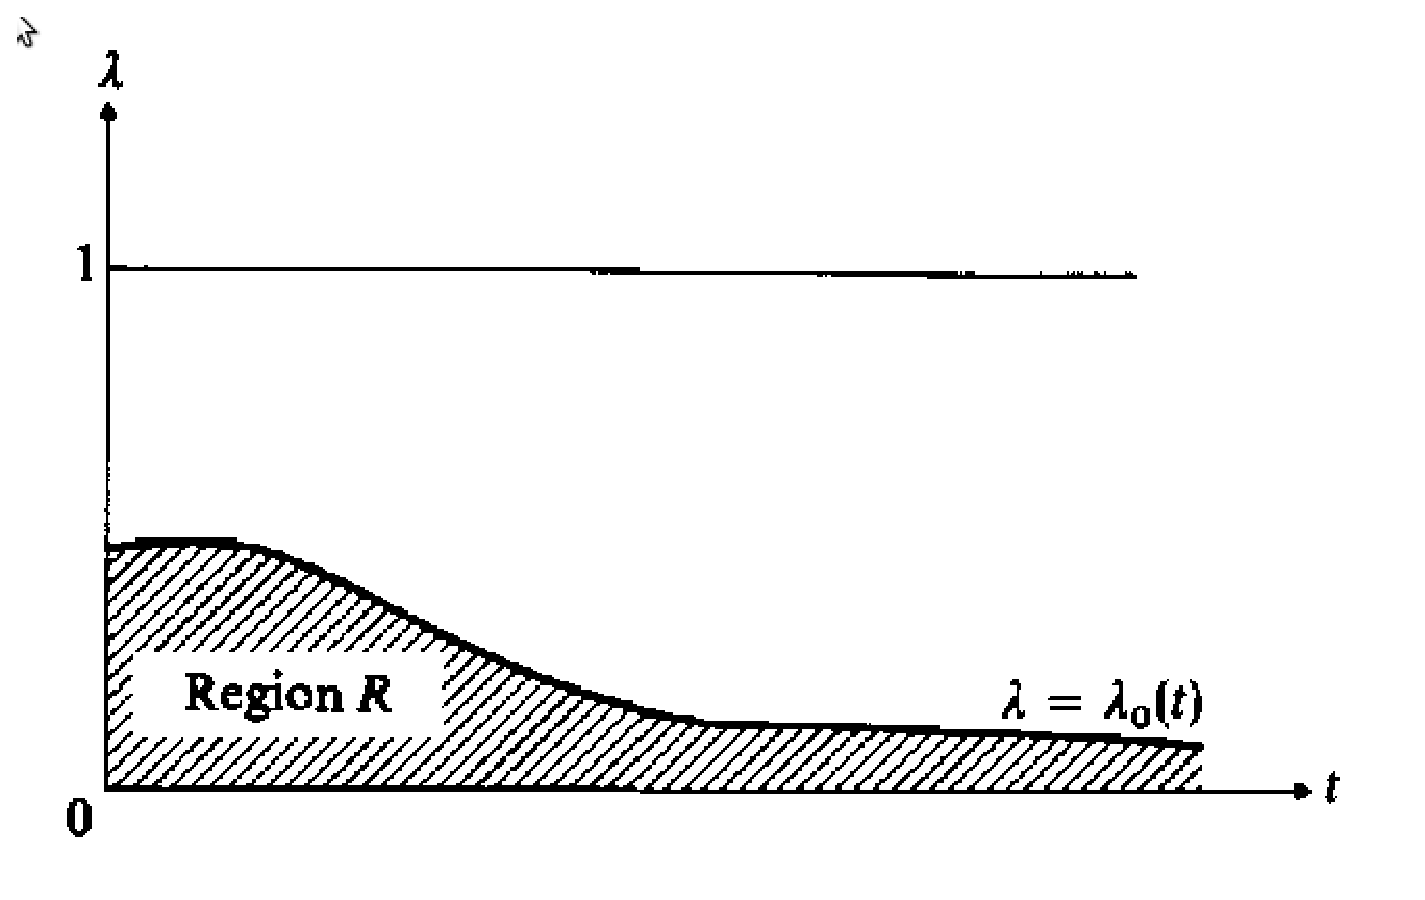
\includegraphics[scale = 0.5]{pictures/critical_region_R.eps}
\caption{Kritický region $R$ vymezený  $\lambda = \lambda_0(t)$ a $\lambda = 0$}
\label{critical-region-R}
\end{figure}
Proto můžeme testovat hypotézu na základě $\Lambda$ podmíněného $T$ - nejprve určíme hodnotu $T$ a následně provede test s pomocí intervalu $0 < \lambda < \lambda_0(t)$ s využitím pravděpodobnosti $\Lambda$ podmíněné $T$. Kritický region tak bude mít podobu plochy namísto intervalu $0 < \lambda < \lambda_0$. Tento region je navíc zkonstruován tak, že bez ohledu na skutečnou hodnotu $\theta$, má chyba typu I stále pravděpodobnost realizace $\alpha$. Připomeňme, že abychom byli schopni aplikovat tento postup, musí existovat dostatečná statistika pro $\theta$.

S využitím výše uvedeného obecného věrohodnostního poměru
\begin{equation*}
\lambda = \frac{\left(\prod_i n_{i \cdot}^{n_{i \cdot}}\right)\left(\prod_j n_{\cdot j}^{n_{\cdot j}}\right)}{n^n \prod_{i,j}n_{ij}^{n_{ij}}}
\end{equation*}
a podmíněných pravděpodobností (9.7) určit interval $0 < \lambda < \lambda_0(n_{i \cdot}; n_{\cdot j})$, který má požadovanou pravděpodobnost chyby typu I pro dané marginální součty. Při aplikaci tohoto testu však narazíme na velmi pracné odvození pravděpodobnostního rozdělení $\Lambda$ pokud $r$, $s$ a marginální součty nejsou relativně malé. Pro dostatečně velké náhodné výběry však lze použít aproximaci s vyjímkou případů, kdy $r$ a $s$ jsou rovny 2, kdy je možné použít specifickou alternativní aproximaci. Tato problematika však přesahuje záběr knihy.

Další test nulové hypotézy $\mathscr{H}_0: p_{ij} = p_{i \cdot} p_{\cdot j}; \sum p_{i \cdot} = 1, \sum p_{\cdot j} = 1$ lze odvodit nahrazením pravděpodobnostního rozdělení v (9.7) vícerozměrnou normální aproximací, kdy lze dokázat, že statistika
\begin{equation*}
Q = \sum_{i,j}\frac{[N_{ij} - n(N_{i \cdot}/n)(N_{\cdot j}/n)]^2}{n(N_{i \cdot}/n)(N_{\cdot j}/n)}
\end{equation*}
přibližně sleduje chi-kvadrát rozdělení s $rs - 1 - (r - 1 + s - 1) = (r - 1)(s - 1)$ stupni volnosti. Test zamítne $\mathscr{H}_0$ pro velká $Q$. Toto kritérium bylo poprvé navrženo Karlem Pearsonem a od $-2 \ln(\lambda)$ se liší členem řádu $1/\sqrt{n}$. Oba testy jsou tak pro dostatečně velké náhodné výběry v podstatě totožné. Statiska $Q$ má intuitivní základ. $N_{ij}$ představuje počet pozorování v $ij$-té buňce dvourozměrné kontingenční tabulky a $n(N_{i \cdot}/n)(N_{\cdot j}/n)$ představuje očekávaný počet pozorování v $ij$-té buňce za předpokladu pravdivosti $\mathscr{H}_0$. Proto dosahuje statistika $Q$ nízkých hodnot pro pravdivé $\mathscr{H}_0$ a vysokých hodnot pro nepravdivé $\mathscr{H}_0$.

\subsubsection{Třírozměrné kontingenční tabulky}

Jestliže lze každý prvek náhodného výběru klasifikovat podle tří kritérií, řekněme $A, B$ a $C$, jsme schopni tyto prvky uspořádat do tzv. třírozměrné kontingenční tabulky. Jestliže kritérium $A$ nabývá hodnot $A_i, i = 1, ..., s_1$, kritérium $B$ hodnot $B_j, j = 1, ..., s_2$ a kritérium $C$ hodnot $C_k, k = 1, ..., s_3$ pak lze tuto kontigenční tabulku chápat jako kvádr, který se skládá z $s_1 \times s_2 \times s_3$ buněk. Pravděpodobnost, že prvek náhodného výběru připadne $ijk$-té buňce označme jako $p_{ijk}$ a počet prvků v této buňce pak jako $N_{ijk}$. Marginální součty budeme, stejně jako v případě dvourozměrné kontingenční tabulky, značit tak, že příslušný index nahradíme znakem $(\cdot)$, tj.
\begin{equation*}
N_{i \cdot k} = \sum_{j = 1}^{s_2}N_{ijk} ~ \textit{a} ~ N_{\cdot \cdot k} = \sum_{i = 1}^{s_1} \sum_{j = 1}^{s_2}N_{ijk}
\end{equation*}
V souvislosti s třírozměrnou kontingenční tabulkou lze testovat čtyři hypotézy. První hypotézou je, že jsou všechna tři kritéria vzájemně nezávislá, tj.
\begin{equation}
\mathscr{H}_0: p_{ijk} = p_{i \cdot \cdot} p_{\cdot j \cdot}  p_{\cdot \cdot k}
\end{equation}
nebo lze testovat zda-li jedno ze tří kritérií je nezávislé na zbývajících dvou kritériích. Např. hypotéza, která testuje nezávislost $B$ na $A$ a $C$, má tvar
\begin{equation}
\mathscr{H}_0: p_{ijk} = p_{i \cdot k} p_{\cdot j \cdot}
\end{equation}
Postup testování těchto hypotéz je analogický postupům v případě dvourozměrných kontingečních tabulek. Věrohodnostní funkce náhodného výběru je
\begin{equation}
L = \prod_{i,j,k} p_{ijk}^{n_{ijk}}
\end{equation}
kde $\sum_{i,j,k} p_{ijk} = 1$ a $\sum_{i,j,k} n_{ijk} = n$. Pro $\overline{\underline{\Theta}}$ nastává maximum $L$ pro $\hat{p}_{ijk} = \frac{n_{ijk}}{n}$, a proto
\begin{equation}
\sup_{\overline{\underline{\Theta}}} L = \frac{1}{n^n}\prod_{i,j,k}n_{ijk}^{n_{ijk}}
\end{equation}
Např. pro testování hypotézy v (9.9) použijeme (9.9) jako substituci do (9.10) a maximalizujeme $L$ s ohledem na $p_{i \cdot k}$ a $p_{\cdot j \cdot}$, čímž získáme
\begin{equation*}
\hat{p}_{i \cdot k} = \frac{n_{i \cdot k}}{n} ~ \textit{a} ~ \hat{p}_{\cdot j \cdot} = \frac{n_{\cdot j \cdot}}{n}
\end{equation*}
a
\begin{equation}
\sup_{\overline{\underline{\Theta}}_0} L = \frac{1}{n^{2n}}\left(\prod_{i,k} n_{i \cdot k}^{n_{i \cdot k}}\right)\left(\prod_j n_{\cdot j \cdot}^{n_{\cdot j \cdot}}\right)
\end{equation}
Příslušný obecný věrohodnostní poměr $\lambda$ je pak dán podílem (9.11) a (9.12) a v případě náhodných výběrů velkého rozsahu je možné jej aproximovat pomocí $-2 \ln(\Theta)$, který sleduje chi-kvadrát rozdělení s $s_1s_2s_3 - 1 - [(s_1s_3 - 1) + s_2 - 1] = (s_1s_3 - 1)(s_2 - 1)$ stupni volnosti. $(s_1s_3 - 1) + (s_2 - 1)$ je dimenze parametrického prostoru $\overline{\underline{\Theta}}_0$ a $s_1s_2s_3 - 1$ je dimenze prostoru $\overline{\underline{\Theta}}$.

Pro hypotézu nezávislosti $B$ na $A$ a $C$, tj.
\begin{equation*}
\mathscr{H}_0: p_{ijk} = p_{i \cdot k} p_{\cdot j \cdot}
\end{equation*}
má odpovídající statistika $Q$ tvar
\begin{equation*}
Q = \sum_i \sum_j \sum_k \frac{[N_{ijk} - n(N_{i \cdot k}/n)(N_{\cdot j \cdot}/n)]^2}{n(N_{i \cdot k}/n)(N_{\cdot j \cdot }/n)}
\end{equation*}
Pro platné $\mathscr{H}_0$ sleduje $Q$ asymptoticky chi-kvadrát rozdělení s $s_1s_2s_3 - 1 - (s_1s_3 - 1) - (s_2 - 1) = (s_1s_3 - 1)(s_2 - 1)$ stupni volnosti. Statistika $Q$ má opět intuitivní základ, protože $N_{ijk}$ představuje počet prvků v buňce $ijk$ a $n(N_{i \cdot k}/n)(N_{\cdot j \cdot}/n)$ představuje očekávaný počet prvků v téže buňce za předpokladu pravdivosti $\mathscr{H}_0$.

\section{Testování hypotéz a intervaly spolehlivosti}

V předchozím textu jsme interval spolehlivosti jednorozměrného parametru $\theta$ použili pro konstrukci testu $\mathscr{H}_0: \theta = \theta_0$ vs. $\mathscr{H}_1: \theta \neq \theta_0$. Tento postup však lze také obrátit a z rodiny testů $\mathscr{H}_0: \theta = \theta_0$ vs. $\mathscr{H}_1: \theta \neq \theta_0$\footnote{Rodinu testů vytvoříme jednoduše tak, že postupně měníme $\theta_0$.} získat interval spolehlivosti pro $\theta$. Následující text je možné chápat jako úvod do problematiky.

Pojem interval spolehlivosti nahraďme obecnějším pojmem množina spolehlivosti. Stejně jako v předchozím textu označuje $\mathfrak{X}$ výběrový prostor, $\overline{\underline{\Theta}}$ parametrický prostor a $(x_1, ..., x_n)$ konkrétní realizaci náhodného výběru.

\begin{definition}[Množina spolehlivosti]
Rodina podmnožin parametrického prostoru $\overline{\underline{\Theta}}$ indexovaná skrze $(x_1, ..., x_n) \in \mathfrak{X}$, kterou označujeme jako $\vartheta =\{\underline{\overline{\Theta}}(x_1, ..., x_n): \overline{\underline{\Theta}}(x_1, ..., x_n) \subseteq \overline{\underline{\Theta}}; (x_1, ..., x_n) \in \mathfrak{X}\}$, je rodinou množin spolehlivosti s koeficietem spolehlivosti $\gamma$, jestliže pro všechna $\theta \in \overline{\underline{\Theta}}$ platí
\begin{equation*}
P_{\theta}[\overline{\underline{\Theta}}(X_1, ..., X_n) ~ \textit{obsahuje} ~ \theta] = \gamma
\end{equation*}
\end{definition}

Libovolný člen $\overline{\underline{\Theta}}(x_1, ..., x_n)$ z rodiny množin spolehlivosti je podmnožinou parametrického prostoru $\overline{\underline{\Theta}}$. $\overline{\underline{\Theta}}(X_1, ..., X_n)$ je náhodnou podmnožinou - pro konkrétní realizaci $(x_1, ..., x_n)$ náhodných veličin $(X_1, ..., X_n)$ nabývá $\overline{\underline{\Theta}}(X_1, ..., X_n)$ hodnoty $\overline{\underline{\Theta}}(x_1, ..., x_n)$, což je člen rodiny $\vartheta$. Pro dané $\theta$ je $\{\overline{\underline{\Theta}}(X_1, ..., X_n) ~ \textit{obsahuje} ~ \theta\}$ náhodným jevem. Toto $\theta$, které taktéž figuruje v $P_{\theta}$ výše uvedené věty, indexuje pravděpodobnostní rozdělení náhodných veličin $(X_1, ..., X_n)$ vystupujících v $\overline{\underline{\Theta}}(X_1, ..., X_n)$.

\begin{example}
Uvažujme náhodný výběr $X_1, ..., X_n$ z populace $N(\theta, 1)$, kde $\overline{\underline{\Theta}} = \{\theta: -\infty < \theta < \infty\}$. Nechť má podmnožina $\overline{\underline{\Theta}}(x_1, ..., x_n)$ podobu intervalu $(\overline{x} - z / \sqrt{n}, \overline{x} + z / \sqrt{n})$, kde $z$ je dáno vztahem $\Phi(z) - \Phi(-z) = \gamma$. Pak je rodina podmnožin $\vartheta = \{\overline{\underline{\Theta}}(x_1, ..., x_n): \overline{\underline{\Theta}}(x_1, ..., x_n) = (\overline{x} - z / \sqrt{n}, \overline{x} + z / \sqrt{n})\}$ rodinou množin spolehlivosti s koeficientem spolehlivosti $\gamma$, protože pro všechna $\theta \in \overline{\underline{\Theta}}$ platí
\begin{multline*}
P_{\theta}[\overline{\underline{\Theta}}(X_1, ..., X_n) ~ \textit{obsahuje} ~ \theta] = P_{\theta}\left[\overline{X} - \frac{z}{\sqrt{n}} < \theta < \overline{X} + \frac{z}{\sqrt{n}}\right]\\
= P_{\theta}\left[-z < \frac{\overline{X} - \theta}{1 / \sqrt{n}} < z \right] = \gamma
\end{multline*}
Rodina $\vartheta$ je rodinou intervalů spolehlivosti pro $\theta$ s koeficientem spolehlivosti $\gamma$.
\end{example}

Jak nyní ukážeme, lze množiny spolehlivosti zkonstruovat na základě testů hypotéz. Uvažujme nenáhodný test $\mathscr{T}_{\theta_0}$ velikosti $\alpha$ pro nulovou hypotézu $\mathscr{H}_0: \theta =  \theta_0$. Nechť $\mathfrak{X}(\theta_0)$ představuje akceptační region testu $\mathscr{T}_{\theta_0}$\footnote{Připomeňme, že akceptační region je doplňkem kritického regionu. Pro kritický region $C(\theta_0)$ tak platí $\mathfrak{X}(\theta_0) = \mathfrak{X} - C(\theta_0)$.}. Protože má test $\mathscr{T}_{\theta_0}$ má velikost $\alpha$ platí
\begin{equation*}
P_{\theta_0}[(X_1, ..., X_n) \in \mathfrak{X}(\theta_0)] = 1 - \alpha
\end{equation*}
S tím, jak měníme $\theta_0$ nad množinou $\overline{\underline{\Theta}}$, získáváme sérii testů $\mathscr{T}_{\theta_0}$ a jim odpovídající akceptačních regiony $\mathscr{X}((\theta_0): \theta_0 \in \overline{\underline{\Theta}}$. Lze definovat
\begin{equation}
\overline{\underline{\Theta}}(x_1, ..., x_n) = \{\theta_0: (x_1, ..., x_n) \in \mathfrak{X}(\theta_0)\}
\end{equation}
Je zřejmé, že $\overline{\underline{\Theta}}(x_1, ..., x_n)$ je podmnožinou $\overline{\underline{\Theta}}$. Dále platí, že $\{\overline{\underline{\Theta}}(x_1, ...,  x_n)\}$ je rodinou množin spolehlivosti s koeficientem spolehlivosti $\gamma = 1 - \alpha$, protože $\{\overline{\underline{\Theta}}(X_1, ..., X_n) ~ \textit{obsahuje} ~ \theta_0\}$ pouze, jestliže $\{(X_1, ..., X_n) \in \mathfrak{X}(\theta_0)\}$, a proto $P_{\theta_0}[\overline{\underline{\Theta}}(X_1, ..., X_n) ~ \textit{obsahuje} ~ \theta_0] = P_{\theta_0}[(X_1, ..., X_n) \in \mathfrak{X}(\theta_0)] = 1 - \alpha$.

\begin{example}
Uvažujme náhodný výběr $X_1, ..., X_n$ z populace $N(\theta, 1)$ a testujme $\mathscr{H_0}: \theta = \theta_0$. Test velikosti $\alpha$ zamítne $\mathscr{H}_0$, jestliže $|\overline{x} - \theta_0| \ge z / \sqrt{n}$, kde $z$ je dáno vztahem $\Phi(z) - \Phi(-z) = 1 - \alpha$. Akceptační region je dán
\begin{equation*}
\mathfrak{X}(\theta_0) = \left((x_1, ..., x_n): \theta_0 - \frac{z}{\sqrt{n}} < \overline{x} < \theta_0 + \frac{z}{\sqrt{n}} \right)
\end{equation*}
Dále, stejně jako v případě (9.13) definujme
\begin{multline*}
\overline{\underline{\Theta}}(x_1, ..., x_n) = \{\theta_0: (x_1, ..., x_n) \in \mathfrak{X}(\theta_0)\}\\
= \left(\theta_0: \theta_0 - \frac{z}{\sqrt{n}} < \overline{x} < \theta_0 + \frac{z}{\sqrt{n}}\right)\\
= \left(\theta_0: \overline{x} - \frac{z}{\sqrt{n}} < \theta_0 < \overline{x} + \frac{z}{\sqrt{n}}\right)
\end{multline*}
$\overline{\underline{\Theta}}(x_1, ..., x_n)$ je interval spolehlivosti s koeficientem spolehlivosti $\gamma = 1 - \alpha$.
\end{example}

Výše uvedený obecný postup ukazuje, jak lze testování hypotéz použít při konstrukci množin spolehlivosti. Tento postup však lze také obrátit a z rodiny množin spolehlivosti získat test hypotézy. Pro rodinu množin spolehlivosti $\{\overline{\underline{\Theta}}(x_1, ..., x_n)\}$ s koeficientem spolehlivosti $\gamma$ jsme definovali
\begin{equation*}
\mathfrak{X}(\theta_0) = \{(x_1, ..., x_n): \theta_0 \in \overline{\underline{\Theta}}(x_1, ..., x_n)\}
\end{equation*}
Nenáhodný test s výše uvedeným akceptačním regionem $\mathfrak{X}(\theta_0)$ je testem hypotézy $\mathscr{H}_0: \theta = \theta_0$ s velikostí $\alpha = 1 - \gamma$.

Vztah mezi testováním hypotéz a množinami spolehlivosti není užitečný pouze k tomu, že z prvního lze odvodit druhé a naopak. Další důležitou oblastí je optimalita testu resp. množiny spolehlivosti. Jestliže je daný test optimální, pak je odpovídající množina spolehlivosti taktéž optimální a naopak. Test toho tvrzení překračuje záběr této knihy, a proto se pouze omezíme na následující definici.

\begin{definition}[Uniformně nejvíce přesná rodina množin spolehlivosti]
Rodina množin spolehlivosti $\{\overline{\underline{\Theta}}^*(x_1, ..., x_n)\}$ s koeficientem spolehlivosti $\gamma$ je uniformně nejpřesnější rodinou množin spolehlivosti pro koeficient $\gamma$, jestliže pro libovolnou alternativní rodinu množin spolehlivosti $\{\overline{\underline{\Theta}}(x_1, ..., x_n)\}$ s koeficientem spolehlivosti $\gamma$ a všechna $\theta$ a $\theta'$ platí
\begin{equation*}
P_{\theta}[\overline{\underline{\Theta}}^*(X_1, ..., X_n) ~ \textit{obsahuje} ~ \theta'] \le P_{\theta}[\overline{\underline{\Theta}}(X_1, ..., X_n) ~ \textit{obsahuje} ~ \theta']
\end{equation*}
\end{definition}

Výše uvedená definice říká, že $\overline{\underline{\Theta}}^*(X_1, ..., X_n)$ obsahuje nesprávné $\theta'$ s menší pravděpodobností než $\overline{\underline{\Theta}}(X_1, ..., X_n)$, přičemž $\overline{\underline{\Theta}}^*(X_1, ..., X_n)$ a $\overline{\underline{\Theta}}(X_1, ..., X_n)$ obsahují správné $\theta$ se stejnou pravděpodobností. Problémem je, že obecné uniformně nejpřesnější množina spolehlivosti zpravidla neexistuje. Nicméně ji lze definovat nad omezeným souborem množin spolehlivosti, kde jsou šance na její existenci větší. K tomuto účelu lze opět využít vztahu mezi testem hypotéz a množinami spolehlivosti. Jestliže je $\mathscr{T}^*$ uniformně nejsilnějším testem velikosti $\alpha$ nad omezeným souborem testů pro hypotézu $\mathscr{H_0}: \theta = \theta_0$, pak je pro tento omezený soubor odpovídající množina spolehlivosti uniformně nejpřesnější s koeficientem $\gamma = 1 - \alpha$. Tímto způsobem lze přetransformovat uniformně nejsilnější test v uniformně nejpřesnější množinu spolehlivosti.

\section{Sekvenční testování hypotéz}

\subsection{Úvod}

Sekvenční testování hypotéz je charakteristické tím, že se velikost náhodného výběru odvíjí od průběhu testu a namísto toho, aby byla dána před samotným testováním. V následujícím textu se zaměříme na jednu z forem sekvenčního testování hypotéz a to na sekvenční pravděpodobnostní poměr.

Uvažujme test ve formě $\mathscr{H}_0: \theta = \theta_0$ vs. $\mathscr{H}_1: \theta = \theta_1$. Dle Neyman-Pearsonovy věty platí, že v případě náhodného výběru velikosti $n$ a chyby typu II velikosti $\alpha$ lze velikost $\beta$ chyby typu I minimalizovat pomocí testu založeného na věrohodnostím poměru. To znamená, že pro dané $\alpha$ a $n$ minimalizujeme $\beta$. Nyní předpokládejme, že pro dané $\alpha$ i $\beta$ chceme stanovit velikost náhodného výběru $n$, pro kterou má odpovídající věrohodnostní poměr chybu I resp. II typu o velikosti $\alpha$ resp. $\beta$. Řešení takovéhoto problému ilustruje následující příklad

\begin{example}
Výrobce ví, že doba živostnosti jeho výrobku je dána $N(100, 100)$. Aby přijal nový výrobní proces, chce si být jistý, že tento proces povede k navýšení střední doby životnosti alespoň o 5\%. K tomuto účelu podrobí testu výrobky z zkušebního provozu, které jsou vyrobeny novým postupem.

Předpokládejme, že doba životnosti výrobku ze zkušebního provozu je $N(\theta, 100)$ a že testujeme $\mathscr{H}_0: \theta \le 100$ vs. $\mathscr{H}_1: \theta > 100$. Zafixujme velikosti chyby typu I a II na 1\% a 5\% a pokusme se nalézt velikost zkušebního vzorku. Platí
\begin{equation*}
0.01 = P_{\theta = 100}[\overline{X}_n > k] ~ \textit{a} ~ 0.05 = P_{\theta = 105}[\overline{X} \le k]
\end{equation*}
neboli
\begin{equation*}
0.01 = 1 - \Phi \left(\frac{k - 100}{10 / \sqrt{n}}\right) ~ \textit{a} ~ 0.05 = \Phi \left(\frac{k - 105}{10 / \sqrt{n}}\right)
\end{equation*}
První z rovnic lze převést do tvaru $\Phi \left(\frac{k - 100}{10 / \sqrt{n}}\right) = 0.99$, což implikuje
\begin{equation*}
\frac{k - 100}{10 / \sqrt{n}} \approx 2.326
\end{equation*}
Druhá rovnice $\Phi \left(\frac{k - 105}{10 / \sqrt{n}}\right) = 0.05$ pak implikuje
\begin{equation*}
\frac{k - 105}{10 / \sqrt{n}} \approx -1.645
\end{equation*}
Jestliže z obou vztahů vyjádříme $k$ a dáme je do rovnosti, získáme
\begin{equation*}
100 + 10 \cdot 2.326 / \sqrt{n} \approx 105 - 10 \cdot 1.645 / \sqrt{n}
\end{equation*}
Řešením je pak $n \approx 63.08$, tj. potřebujeme vzorek o velikosti 64 výrobků.
\end{example}

Ve výše uvedeném případě nemusí být vždy nutné otestovat všech 64 výrobků, abychom byli schopni přijmout či zamítnout nulovou hypotézu. Může se totiž stát, že již během prvních 20, 30 či 40 pozorování získáme dostatečné důkazy k tomu, abychom pro dané $\alpha$ a $\beta$ nulovou hypotézy přijali popř. zamítli. To znamená, že je zde možnost zkonstruovat takový test, který by v průměru umožnil ukončit testování před dosažením počtu 64 pozorování. Tímto se dostáváme k následující kapitole.

\subsection{Definice sekvenčního poměrového testu}

Uvažujme dvě populace a náhodný výběr, o kterém nevíme, ze které populace pochází. Předpokládejme, že naším cílem je tento náhodný výběr přiřadit jedné z populací. Testujeme tedy $\mathscr{H}_0: X_i ~ f_0(\cdot)$ vs. $\mathscr{H}_1: X_i ~ f_1(\cdot)$. Připomeňme, že věrohodnostní poměrový test zamítl $\mathscr{H}_0$, jestliže
\begin{equation*}
\lambda = \frac{L_0}{L_1} \le k
\end{equation*}
pro určitou konstantu $k > 0$. Sekvenční poměrový test je založen na sérii takovýchto testů. Definujme
\begin{equation*}
\lambda_m = \lambda_m(x_1, ..., x_m) = \frac{L_0(x_1, ..., x_m)}{L_1(x_1, ..., x_m)} = \frac{L_0(m)}{L_1(m)} = \frac{\prod_{i = 1}^m f_0(x_i)}{\prod_{i = 1}^m f_1(x_i)}
\end{equation*}
pro $m = 1, 2 , ...$ a postupně vypočtěme $\lambda_1, \lambda_2, ...$. Pro fixní $k_0$ a $k_1$, které splňují podmínku $0 < k_0 < k_1$, aplikujme následující postup.
\begin{enumerate}
\item Realizujeme pozorování $x_1$ a vypočteme pro něj poměr $\lambda_1$.
\item Jestliže $\lambda_1 \le k_0$, zamítneme $\mathscr{H}_0$ a ukončíme testování.
\item Jestliže $\lambda_1 \ge k_1$, přijmeme $\mathscr{H}_0$ a ukončíme testování.
\item Jestliže $k_0 < \lambda_1 < k_1$, realizujeme pozorování $x_2$ a vypočteme $\lambda_2$.
\item Jestliže $\lambda_2 \le k_0$, zamítneme $\mathscr{H}_0$ a ukončíme testování.
\item Jestliže $\lambda_2 \ge k_1$, přijmeme $\mathscr{H}_0$ a ukončíme testování.
\item Jestliže $k_0 < \lambda_2 < k_1$, realizujeme pozorování $x_3$ a vypočteme $\lambda_3$.
\item Postupně navyšujeme počet pozorování a aplikujeme výše popsaný postup, dokud
\begin{enumerate}
\item $\lambda_i \le k_0$, kdy zamítneme $\mathscr{H}_0$ a ukončíme testování
\item $\lambda_i \ge k_1$, kdy přijmeme $\mathscr{H}_0$ a ukončíme testování
\end{enumerate}
\end{enumerate}
Kritický region výše popsaného sekvenčního testu je $C = \cup_{n = 1}^{\infty}C_n$, kde
\begin{equation*}
C_n = \{(x_1, ..., x_n): k_0 < \lambda_j(x_1, ..., x_j) < k_1, j = 1, ..., n -1, \lambda_n(x_1, ..., x_n) \le k_0\}
\end{equation*}
Podobně akceptační region je $A = \cup_{n = 1}^{\infty} A_n$, kde
\begin{equation*}
A_n = \{(x_1, ..., x_n): k_0 < \lambda_j(x_1, ..., x_j) < k_1, j = 1, ..., n - 1, \lambda_n(x_1, ..., x_n) \ge k_1\}
\end{equation*}

\begin{definition}[Sekvenční poměrový test]
Pro dané $0 < k_0 < k_1$ je výše popsaný test označován jako sekvenční poměrový test.
\end{definition}

V předchozím textu jsme se pro dané $n$ snažili stanovit $k$ tak, aby výsledný test měl velikost $\alpha$. Nyní se pokusíme stanovit $k_0$ a $k_1$ takové, aby výsledný sekvenční poměrový test měl chyby typu I resp. II předem dané velikosti $\alpha$ resp. $\beta$. Všimněme si, že
\begin{equation*}
\alpha = P[\textit{zamítnutí} ~ \mathscr{H}_0 | \mathscr{H}_0 je pravdivé] = \sum_{n = 1}^{\infty} \int_{C_n} L_0(n)
\end{equation*}
a
\begin{equation*}
\beta = P[\textit{přijetí} ~ \mathscr{H}_0 | \mathscr{H}_0 je nepravdivé] = \sum_{n = 1}^{\infty} \int_{A_n} L_1(n)
\end{equation*}
kde, stejně jako dříve, představuje $\int_{C_n} L_0(n)$ zkrácený zápis pro $\int \cdots \int_{C_n}\left(\prod_{i = 1}^n f_0(x_i)dx_i\right)$. Protože $A_n$ a $C_n$ jsou vyjádřeny ve formě $k_0$ a $k_1$, lze pro fixní $\alpha$ a $\beta$ výše uvedené dvě rovnice chápat jako rovnice o dvou neznámých $k_0$ a $k_1$. Jejich řešením pak získáme sekvenční poměrový test s chybami o velikosti $\alpha$ a $\beta$. Jak je však při pohledu na tyto dvě rovnice patrné, je výpočet $k_0$ a $k_1$ poměrně komplikovanou záležitostí. Naštěstí však existuje poměrně jednoduchá aproximace, kterou si představíme následující kapitole.

V rámci sekvečního poměrového testu navyšujeme počet pozorování, dokud se $\lambda_n(x_1, ..., x_n)$ nenachází mimo interval $(k_0, k_1)$. Velikost náhodného vzorku v rámci testu tak závisí na realizacích $x_1, x_2, ...$ náhodných veličin $X_1, X_2, ...$, a proto se jedná taktéž o náhodnou veličinu. Označme ji písmenem $N$. Jedním ze způsobů hodnocení sekvenčních poměrových testů je porovnání střední hodnoty $N$, kde preferujeme test s nižší střední hodnotou. Tímto se dostáváme k následující větě, kterou uvádíme bez důkazu.

\begin{theorem}
Sekvenční poměrový test, který splňuje
\begin{equation*}
P[\mathscr{H}_0 ~ \textit{je zamítnuto}| \mathscr{H_0} ~ \textit{je pravdivé}] \le \alpha
\end{equation*}
a
\begin{equation*}
P[\mathscr{H}_0 ~ \textit{je přijmuto}| \mathscr{H_0} ~ \textit{je nepravdivé}] \le \beta
\end{equation*}
minimalizuje v porovnání se všemi alternativními testy s chybami velikosti $\alpha$ a $\beta$ jak
\begin{equation*}
E[N|\mathscr{H}_0 ~ \textit{je pravdivé}]
\end{equation*}
tak
\begin{equation*}
E[N|\mathscr{H}_0 ~ \textit{je nepravdivé}]
\end{equation*}
V tomto směru je tedy tento sekvenční poměrový test optimální.
\end{theorem}

\subsection{Přibližný sekvenční poměrový test}

V předchozím textu jsme konstatovali, že výpočet parametrů $k_0$ a $k_1$, které jsou nezbytné pro definování sekvenčního poměrového testu, je poměrně komplikovaný. Naštěstí existuje relativně jednoduchá aproximace těchto parametrů.

\begin{corollary}
Nechť jsou $k_0$ a $k_1$ definovány tak, že jim odpovídající sekvenční poměrový test má chyby velikosti $\alpha$ a $\beta$. Parametry $k_0$ a $k_1$ lze aproximovat pomocí
\begin{equation*}
k_0' = \frac{\alpha}{1 - \beta} ~~~ \textit{a} ~~~ k_1' = \frac{1 - \alpha}{\beta}
\end{equation*}
\end{corollary}

\begin{proof}
Předpokládejme, že $\sum_{n = 1}^{\infty} P[N = n|\mathscr{H}_i] = 1$ pro $i = 0, 1$. Z definice chyby typu I a poměrového testu vyplývá
\begin{multline*}
\alpha = P[\textit{zamítnutí} ~ \mathscr{H}_0 | \mathscr{H}_0 ~ \textit{je pravdivé}] = \sum_{n = 1}^{\infty} \int_{C_n}L_0(n) \le \sum_{n = 1}^{\infty} \int_{C_n} k_0 L_1(n)\\
= k_0 \sum_{n = 1}^{\infty} \int_{c_n} L_1(n) = k_0 P[\textit{zamítnutí} ~ \mathscr{H}_0 | \mathscr{H}_1 ~ \textit{je pravdivé}] = k_0 (1 - \beta)
\end{multline*}
a proto $k_0 \ge \frac{\alpha}{1 - \beta}$. Zároveň však také platí
\begin{multline*}
1 - \alpha = P[\textit{přijetí} ~ \mathscr{H}_0 | \mathscr{H}_0 ~ \textit{je pravdivé}] = \sum_{n = 1}^{\infty} \int_{A_n} L_0(n) \ge \sum_{n = 1}^{\infty} \int_{A_n} k_1 L_1(n)\\
= k_1 P[\textit{přijetí} ~ \mathscr{H}_0 | \mathscr{H}_1 ~ \textit{je pravdivé}] = k_1 \beta
\end{multline*}
a proto $k_1 \le \frac{1 - \alpha}{\beta}$. Všimněme si, že aproximace $k_0' = \frac{\alpha}{1 - \beta}$ a $k_1' = \frac{1 - \alpha}{\beta}$ splňují
\begin{equation*}
k_0' = \frac{\alpha}{1 - \beta} \le k_0 < k_1 \le \frac{1 - \alpha}{\beta} = k_1'
\end{equation*}
\end{proof}

\begin{corollary}
Jestliže jsou $\alpha'$ a $\beta'$ velikosti chyb sekvenčního poměrového testu definovaného pomocí $k_0'$ a $k_1'$, pak platí $\alpha' + \beta' \le \alpha + \beta$.
\end{corollary}

\begin{proof}
Nechť $A'$ resp. $C'$ označuje akceptační resp. kritický region sekvenčního poměrového testu definovaného pomocí $k_0'$ a $k_1'$. Pak platí
\begin{equation*}
\alpha' = \sum_{n = 1}^{\infty} \int_{C_n'} L_0(n) \le \frac{\alpha}{1 - \beta} \sum_{n = 1}^{\infty} \int_{C_n'}L_1(n) = \frac{\alpha}{1 - \beta}{1 - \beta'}
\end{equation*}
a
\begin{equation*}
1 - \alpha' = \sum_{n = 1}^{\infty} \int_{A_n'} L_0(n) \ge \frac{1 - \alpha}{\beta} \sum_{n = 1}^{\infty}\int_{A_n'}L_1(n) = \frac{1 - \alpha}{\beta} \beta'
\end{equation*}
a proto $\alpha'(1 - \beta) \le \alpha(1 - \beta')$ a $(1 - \alpha)\beta' \le (1 - \alpha')\beta$, což v souhrnu implikuje $\alpha'(1 - \beta) + (1 - \alpha)\beta' \le \alpha(1 - \beta') + (1 - \alpha')\beta$ neboli $\alpha' + \beta' \le \alpha + \beta$.
\end{proof}

Ideálně bychom preferovali sekvenční poměrový test, který má chyby o předem daných velikostech $\alpha$ a $\beta$. Protože je však složité nalézt odpovídající $k_0$ a $k_1$, použijeme testt definovaný pomocí jejich aproximací $k_0'$ a $k_1'$ s vědomím, že součet chyb $\alpha'$ a $\beta'$ je menší nebo roven součtu požadovaných chyb $\alpha$ a $\beta$.

\subsection{Přibližná střední hodnota velikosti náhodného výběru sekvenčního poměrového testu}

Sekvenční poměrový test probíhá tak dlouho, dokud $k_0 < \lambda_m < k_1$ a skonční jakmile $\lambda_m \le k_0$ nebo $\lambda_m \ge k_1$. Definujme $z_i = \ln \left(\frac{f_0(x_i)}{f_1(x_i)}\right)$. V rámci ekvivalentního testu pak navyšujeme velikost vzorku dokud $\ln(k_0) < \sum_{i = 1}^m z_i < \ln(k_1)$ a test ukončíme, jestliže $\sum_{i = 1}^m z_i \le \ln(k_0)$, kdy $\mathscr{H}_0$ zamítneme, nebo $\sum_{i = 1}^m z_i \ge \ln(k_1)$, kdy $\mathscr{H}_0$ přijmeme. Stejně jako v předchozím textu i zde představuje náhodná veličina $N$ velikost vzorku sekvenčního poměrového testování. Dále definujme $Z_i = \ln\left(\frac{f_0(X_i)}{f_1(X_i)}\right)$. Následující věta slouží k určení přibližné střední hodnoty velikosti výběru pro sekvenční poměrový test.

\begin{theorem}[Waldova rovnice]
Uvažujme nezávislé náhodné veličiny $Z_1, ..., Z_n, ...$ s identickým pravděpodobnostním rozdělením. Nechť tyto náhodné veličiny splňují podmínku $E[|Z_i| < \infty]$ a nechť $N$ je náhodná veličina, která nabývá hodnot z oboru přirozených čísel. Pak platí
\begin{equation*}
E[Z_1 + ... + Z_n] = E[N] \cdot E[Z_i]
\end{equation*}
\end{theorem}

\begin{proof}
\begin{multline*}
E[Z_1 + ... + Z_N] = E[E[Z_1 + ... + Z_N] | N]\\
= \sum_{n = 1}^{\infty} E[Z_1 + ... + Z_n| N = n] P[N = n] = \sum_{n = 1}^{\infty} \sum_{i = 1}^n E[Z_i|N = n]P[N = n]\\
= \sum_{i = 1}^{\infty} \sum_{n = 1}^{\infty} E[Z_i|N = n]P[N = n] = \sum_{i = 1}^{\infty} E[Z_i|N \ge i]P[N \ge i]\\
= \sum_{i = 1}^{\infty}E[Z_i]P[N \ge i] = E[Z_i]\sum_{i = 1}^{\infty}P[N \ge i] = E[Z_i] E[N]
\end{multline*}
Při úpravách jsme použili vztah $E[Z_i] = E[Z_i|N \ge i]$. Tento vztah platí, protože $\{N \ge i\}$ závisí pouze na $Z_1, ..., Z_{i - 1}$, a proto je nezávislý na $Z_i$. Vztah $E[N] = \sum_{i = 1}^{\infty}P[N \ge i]$ pak vychází z bodu (3) definice střední hodnoty (2.11).
\end{proof}

Jestliže sekvenční pravděpodobnostní test vede k zamítnutí $\mathscr{H}_0$, pak $Z_1 + ... + Z_N \le \ln(k_0)$, nicméně $Z_1 + ... + Z_N$ je relativně blízké $\ln(k_0)$, protože $Z_1 + ... + Z_N$ se stane poprvé menší nebo rovno $\ln(k_0)$ pro $N$-té pozorování. Proto platí $E[Z_1 + ... + Z_N] \approx \ln(k_0)$. Podobně, jestliže test vede k přijetí $\mathscr{H}_0$, platí $E[Z_1 + ... + Z_n] \approx \ln(k_1)$. Proto $E[Z_1 + ... + Z_N] \approx \rho \ln(k_0) + (1 - \rho)\ln(k_1)$, kde $\rho = P[\mathscr{H}_0 ~ \textit{je zamítnuto}]$. S využitím
\begin{equation*}
E[N] = \frac{E[Z_1 + ... + Z_N]}{E[Z_1]} \approx \frac{\rho \ln(k_0) + (1 - \rho)\ln(k_1)}{E[Z_i]}
\end{equation*}
získáme
\begin{multline}
E[N | \mathscr{H}_0 ~ \textit{je pravdivé}] \approx \frac{\alpha \ln(k_0) + (1 - \alpha)\ln(k_1)}{E[Z_i|\mathscr{H}_0 ~ \textit{je pravdivé}]}\\
\approx \frac{\alpha \ln[\alpha / (1 - \beta)] + (1 - \alpha)\ln[(1 - \alpha) / \beta]}{E[Z_i | \mathscr{H}_0 ~ \textit{je pravdivé}]}
\end{multline}
a
\begin{multline}
E[N | \mathscr{H}_0 ~ \textit{je nepravdivé}] \approx \frac{(1 - \beta) \ln(k_0) + \beta \ln(k_1)}{E[Z_i|\mathscr{H}_0 ~ \textit{je nepravdivé}]}\\
\approx \frac{(1 - \beta) \ln[\alpha / (1 - \beta)] + \beta \ln[(1 - \alpha) / \beta]}{E[Z_i | \mathscr{H}_0 ~ \textit{je nepravdivé}]}
\end{multline}

\begin{example}
Uvažujme náhodný výběr z $N(\theta, \sigma^2)$, kde $\sigma^2$ známe. Testujme $\mathscr{H}_0> \theta = \theta_0$ vs. $\mathscr{H}_1: \theta = \theta_1$. Platí
\begin{multline*}
z_i = \ln \left(\frac{f_0(x_i)}{f_1(x_i)}\right) = \ln \left(\frac{(1 / \sqrt{2 \pi} \sigma)e^{-\frac{1}{2}[(x_i - \theta_0)/\sigma]^2}}{(1 / \sqrt{2 \pi} \sigma)e^{-\frac{1}{2}[(x_i - \theta_0)/\sigma]^2}}\right)\\
= - \frac{1}{2 \sigma^2}[(x_i - \theta_0)^2 - (x_i - \theta_1)^2] = -\frac{1}{2 \sigma^2}[(\theta_0^2 - \theta_1^2) - 2x_i(\theta_0 - \theta_1)]
\end{multline*}
a proto
\begin{equation*}
E[Z_i | \mathscr{H}_0 ~ \textit{je pravdivé}] = -\frac{1}{2 \sigma^2}[(\theta_0^2 - \theta_1^2) - 2 \theta_0(\theta_0 - \theta_1)] = \frac{1}{2 \sigma^2}(\sigma_1 - \sigma_0)^2
\end{equation*}
a
\begin{equation*}
E[Z_i | \mathscr{H}_0 ~ \textit{je nepravdivé}] = - \frac{1}{2 \sigma^2}(\theta_1 - \theta_0)^2
\end{equation*}
Vraťme se k příkladu (9.27). Dle zadání tohoto příkladu je $\alpha = 0.01, \beta = 0,05, \sigma^2 = 100, \theta_0 = 100$ a $\theta_1 = 105$. Dosazením do (9.14) a (9.15) získáváme
\begin{equation*}
E[N|\mathscr{H}_0 ~ \textit{je pravdivé}] \approx \frac{0.01 \ln(0.01 / 0.95) + 0.99 \ln(0.99 / 0.05)}{25 / 200} \approx 24
\end{equation*}
a
\begin{equation*}
E[N | \mathscr{H}_0 ~ \textit{je nepravdivé}] \approx 34
\end{equation*}
Pro sekvenční poměrový test jsou tedy průměrné velikosti vzorku 24 resp. 34 výrobků. Pro test s pevně danou velikostí vzorku jsem v příkladě (9.27) dospěli k počtu 64 produktů. 
\end{example}
